\chapter{A Numerical Evaluation of the PEM} \label{ch:results}
%
This chapter provides a detailed numerical assessment of the DG-PEM and its variants. Investigations into the sensitivity of the 

\section{Irons' Patch Tests}

In this section we investigate the behavior of PEM elements in the context of the standard Iron's patch test, whose passage is argued to be a necessary and sufficient condition for convergence in \cite{Simo&Taylor:86} (though this claim has been disputed, namely by Stummel in \cite{Stummel:80}).

Two tests will be considered: the linear and quadratic patch tests, as depicted in figure \ref{fig:polygonal_patches}. 

\begin{figure}[!h]
    \centering
    \begin{subfigure}[b]{0.49\linewidth}
            \centering
            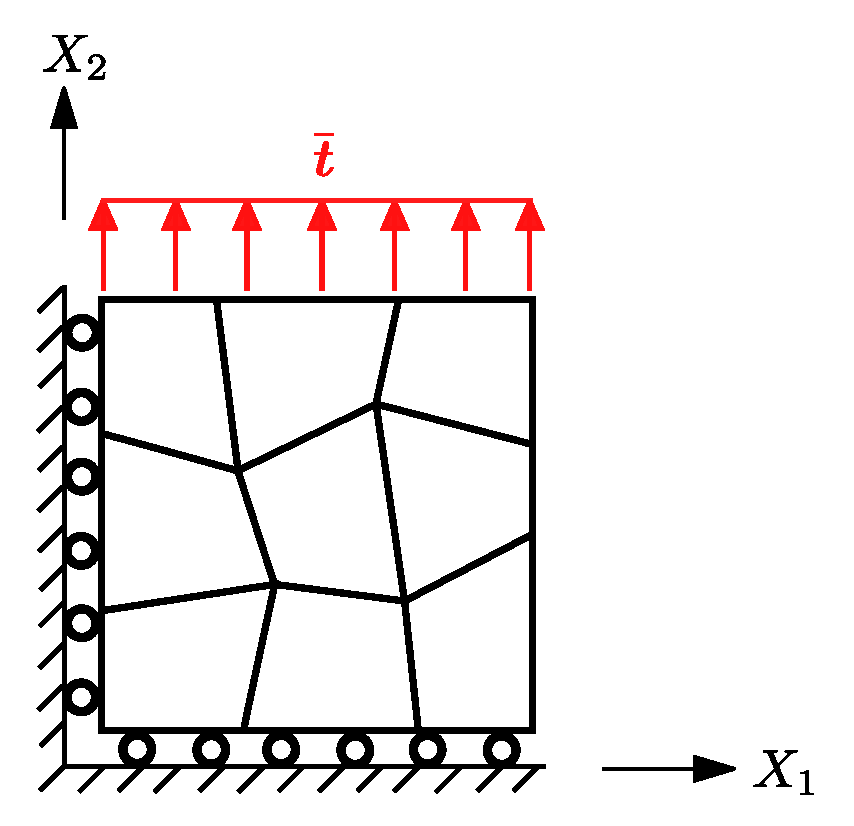
\includegraphics[width=2.0in]{figures/linear_patch_test.pdf}
    			\caption{linear patch test \label{fig:linear_patch_test}}
    \end{subfigure}
	\begin{subfigure}[b]{0.49\linewidth}
            \centering
            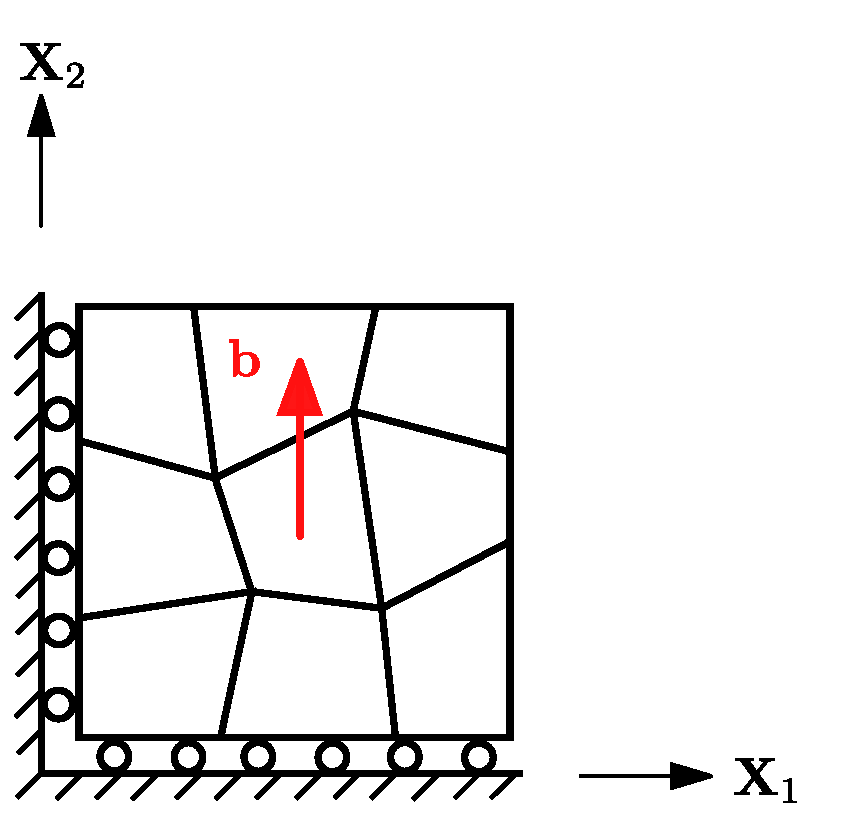
\includegraphics[width=2.0in]{figures/quadratic_patch_test.pdf}
    			\caption{quadratic patch test \label{fig:quadratic_patch_test}}
    \end{subfigure}
    \caption{Depiction of simple patch tests for (\subref{fig:linear_patch_test}) linear and (\subref{fig:quadratic_patch_test}) quadratic elements.}
    \label{fig:polygonal_patches}
\end{figure}

Want to show a series of problems which link:
1) parameter choice to poor condition number
2) poor condition number to interpolation error
3) interpolation error to patch test errors

Need a way to compute interpolation error (and possibly integration error) for arbitrary patches...
Consider: specifying all nodal values to be consistent with a univariate polynomial (in Ux displacement, only; in terms of stuff)
Set the material as E = 1.0, nu = 0.0, such that we recover stresses as strains via identity mapping
Compute error directly as L2 and H1 norms; each will give error in representing the field and its gradient.
In other words: constrain all nodes; any error is attributable to integration error

\section{Element Quality and Parameter Sensitivity}

\subsection{Meshes Consisting of Elements with Degenerate Edges}

Consider the two square patches depicted in Figure \ref{fig:polygonal_patches}, each containing 1,000 polygonal elements. Both meshes were generated using the PolyMesher, a polygonal meshing tool detailed in \cite{Talischi:12}; the mesh in Figure \ref{fig:patch_mesh} . As noted in the figure, the resulting elements may possess extremely short edges, which can potentially degrade the quality of any finite element solution computed on the polygonal mesh. Herein, we will investigate the effects of having short edges within a given mesh.
\begin{figure}[!h]
    \centering
    \begin{subfigure}[b]{0.49\linewidth}
            \centering
            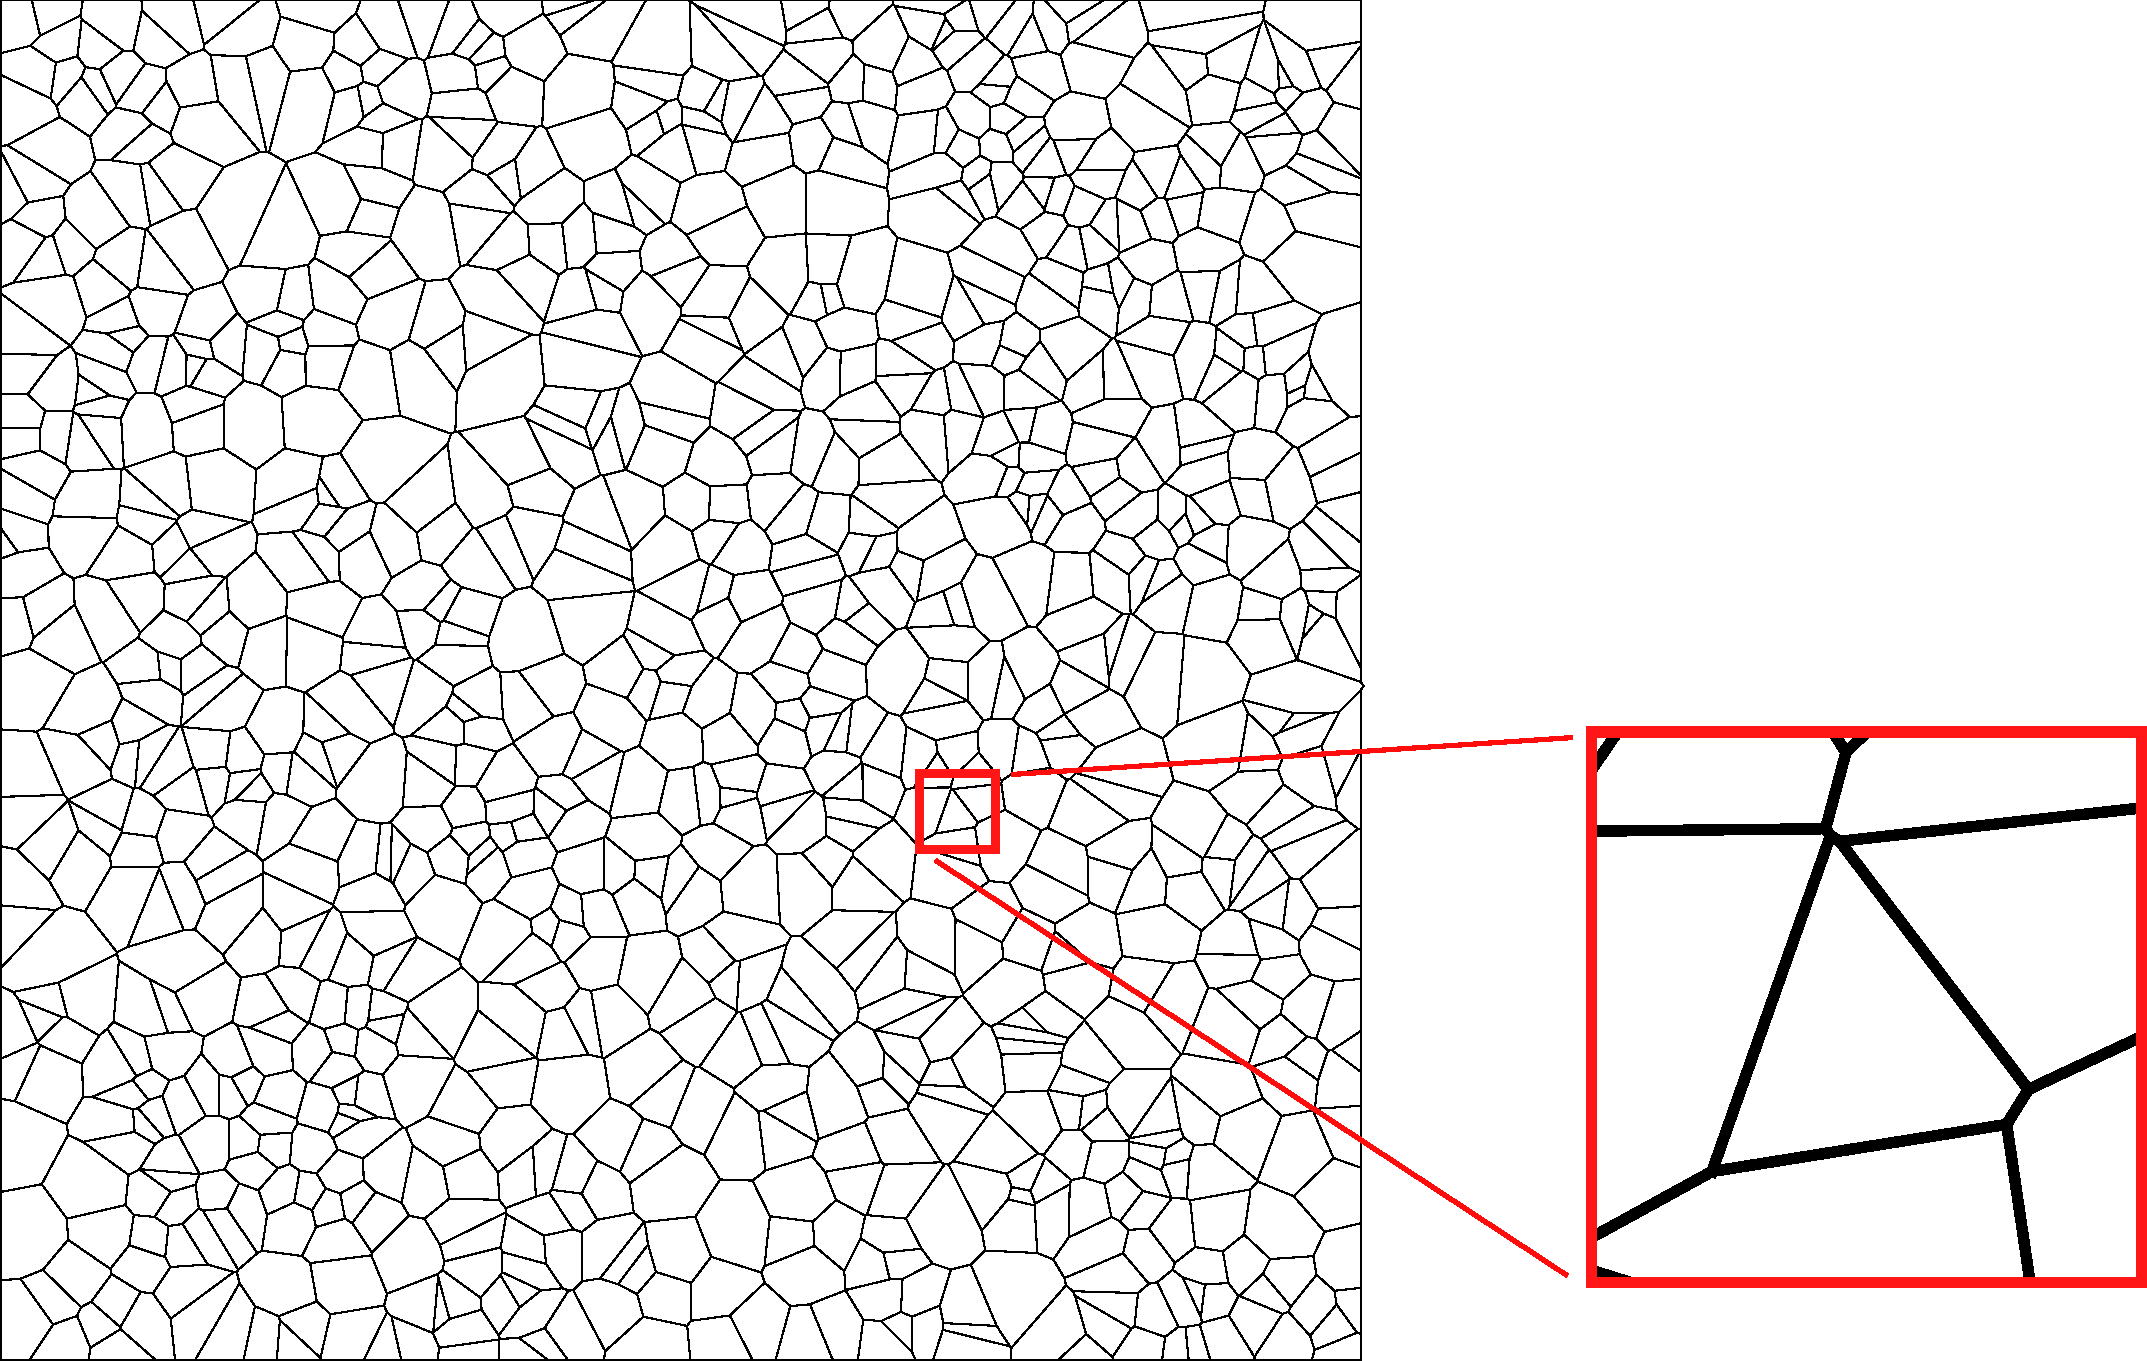
\includegraphics[width=3.0in]{figures/patch_mesh.pdf}
    			\caption{Random Voronoi mesh \label{fig:patch_mesh}}
    \end{subfigure}
	\begin{subfigure}[b]{0.49\linewidth}
            \centering
            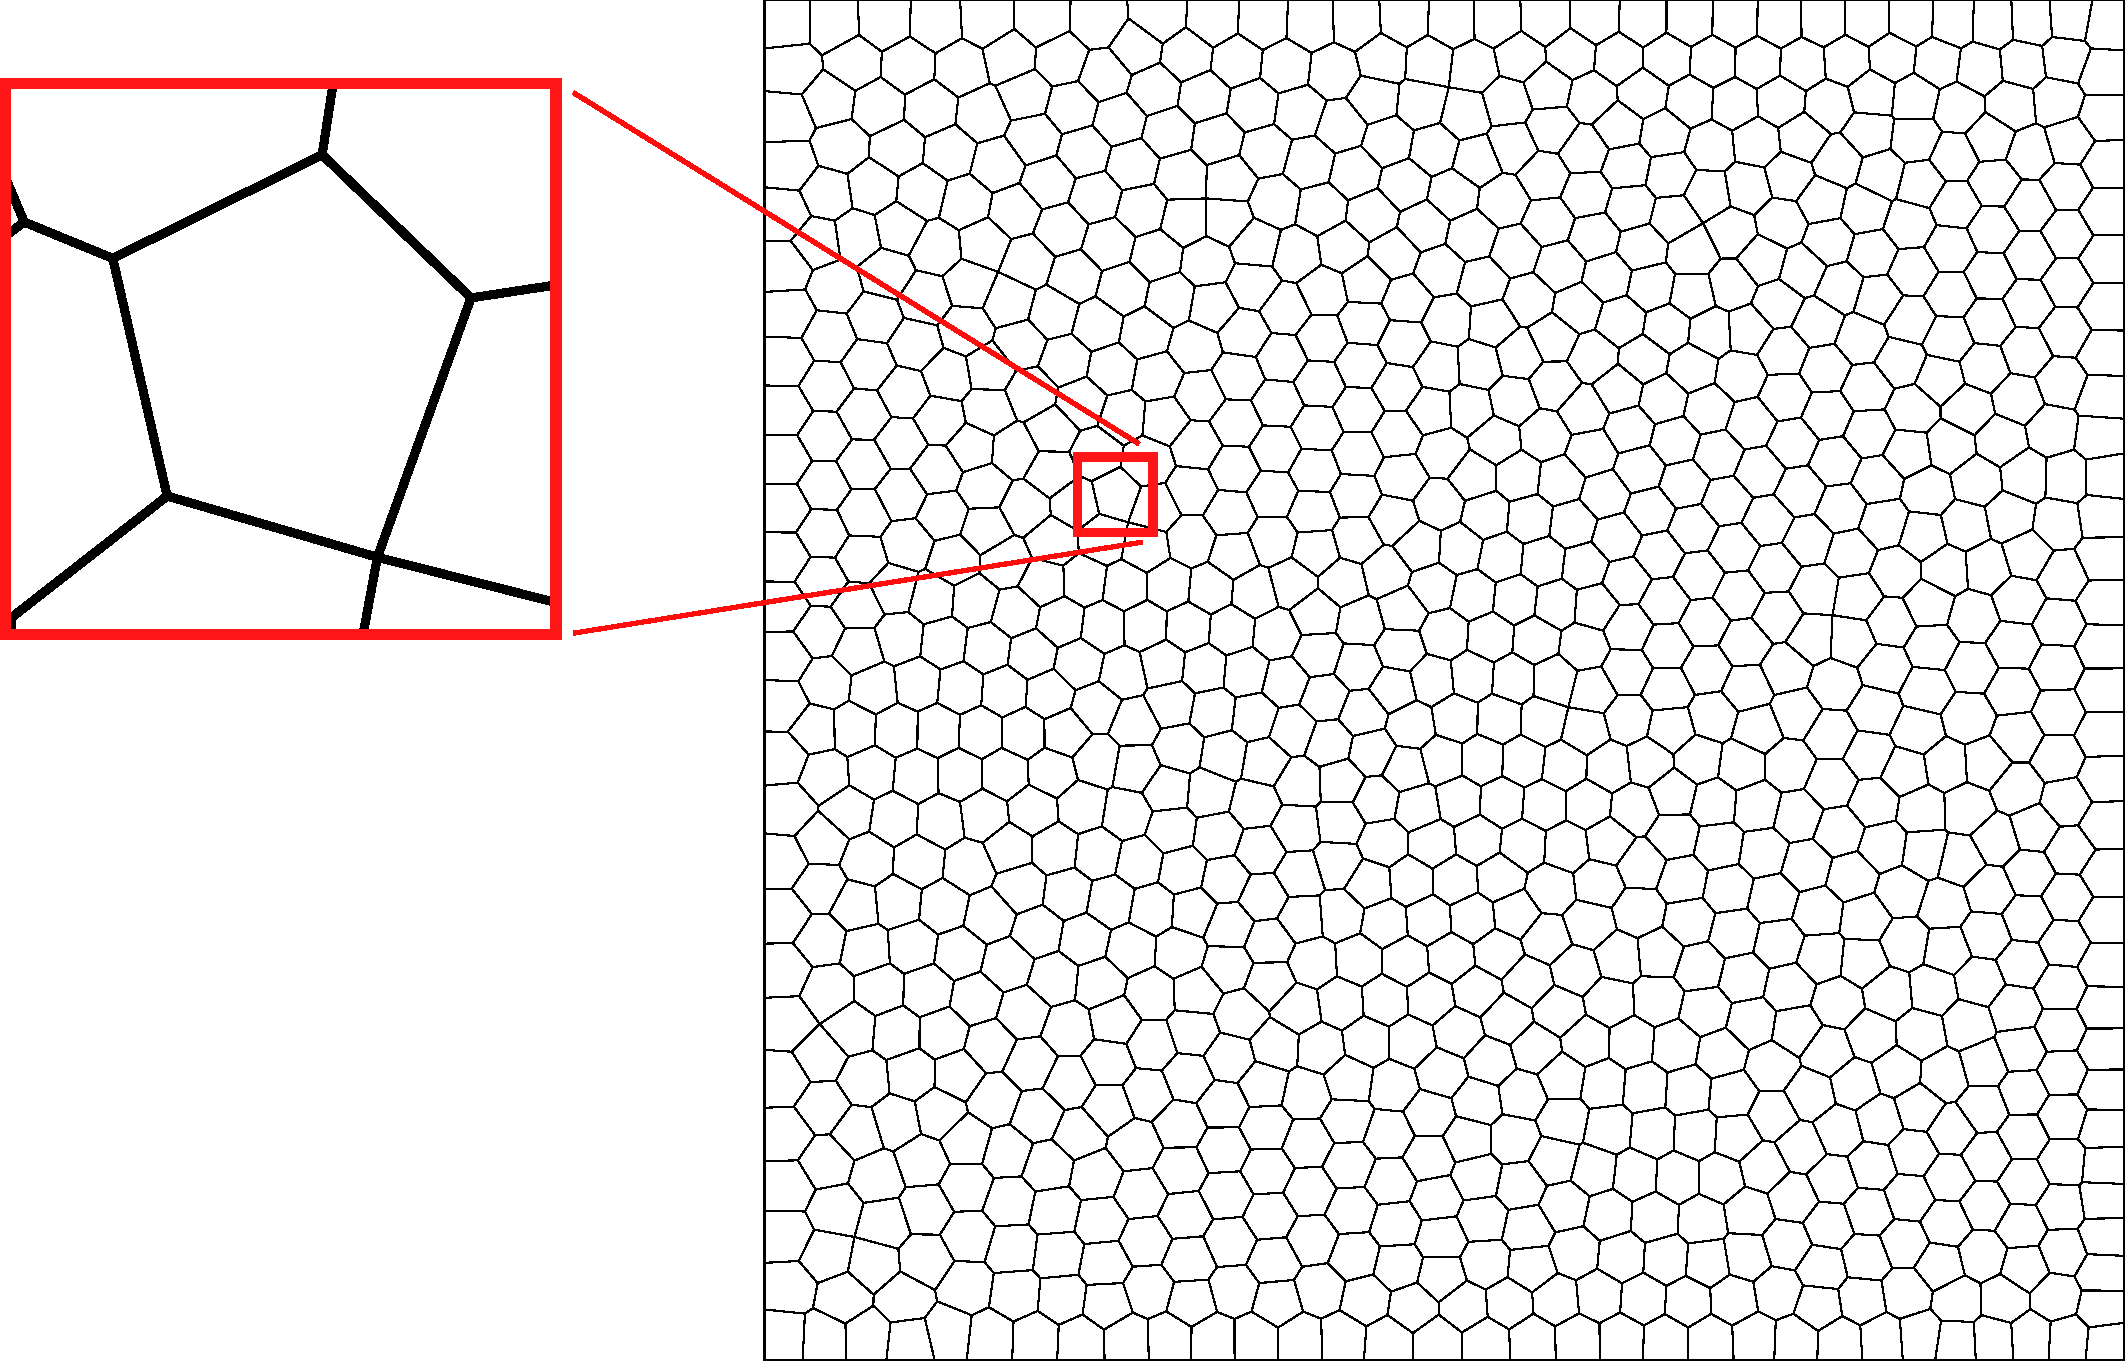
\includegraphics[width=3.0in]{figures/lloyd_mesh.pdf}
    			\caption{Lloyd mesh (100 iterations) \label{fig:lloyd_mesh}}
    \end{subfigure}
    \caption{Patches generated by PolyMesher, each containing 1,000 polygonal elements.}
    \label{fig:polygonal_patches}
\end{figure}

Some preliminary definitions are provided. For every polygonal element $\Omega_e \subset \mathbb{R}^2$, let $h_e$ denote the diameter of $\Omega_e$, such that
\begin{equation}
	h_e = \sup_{\mathbf{X}_1, \mathbf{X}_2 \in \Omega_e} || \mathbf{X}_1 - \mathbf{X}_2 ||_2.
\end{equation}
Further, denote by $|E|$ the length of any edge $E \subset \partial \Omega_e$, and define $\rho_e$ as the ratio of the smallest edge length $|E|$ divided by the element diameter $h_e$, i.e.
\begin{equation}
	\rho_e = \max_{E \subset \partial \Omega_e} \frac{|E|}{h_e}.
\end{equation}

For the mesh depicted in \ref{fig:polygonal_patches}, 
\begin{figure}[!h]
    \centering
    \begin{subfigure}[b]{0.49\linewidth}
            \centering
            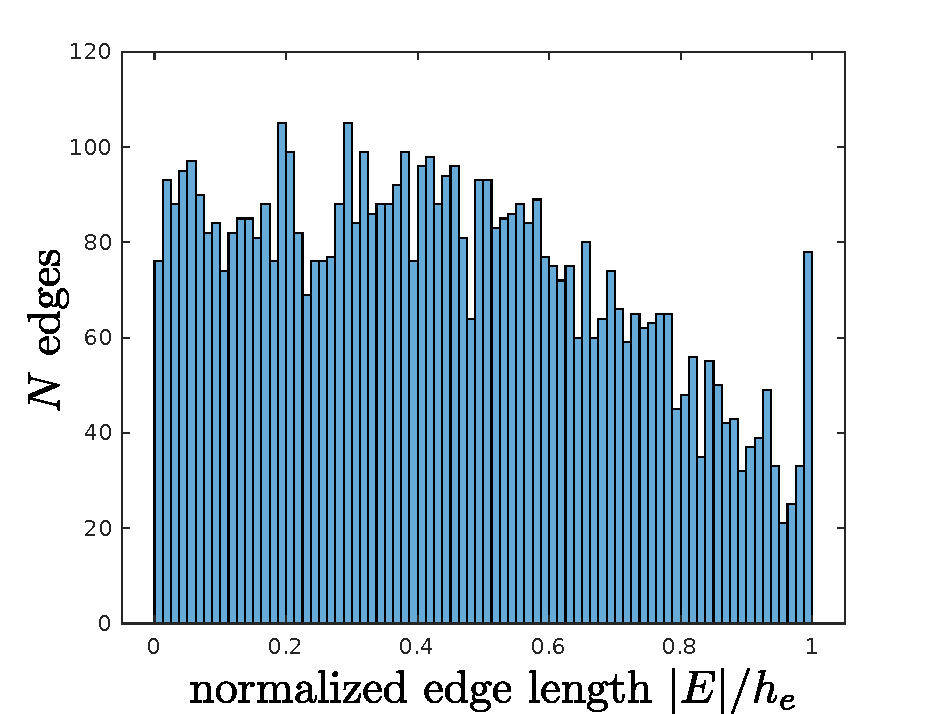
\includegraphics[width=3.0in]{figures/patch_edge_lengths.pdf}
    			\caption{Voronoi mesh \label{fig:patch_edge_lengths}}
    \end{subfigure}
	\begin{subfigure}[b]{0.49\linewidth}
            \centering
            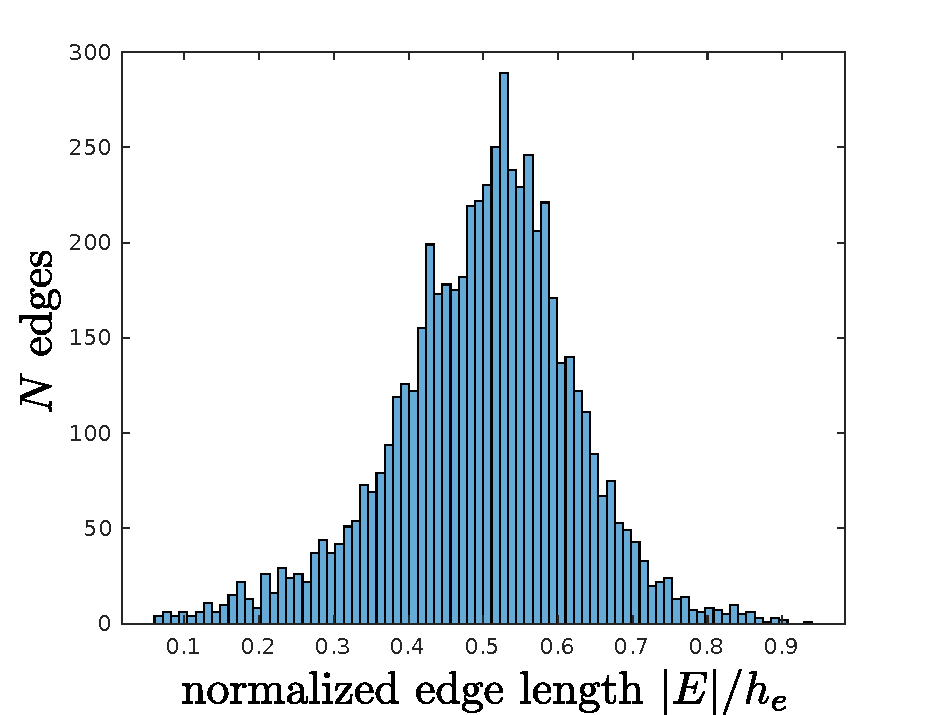
\includegraphics[width=3.0in]{figures/lloyd_edge_lengths.pdf}
    			\caption{Lloyd mesh \label{fig:lloyd_edge_lengths}}
    \end{subfigure}
    \begin{subfigure}[b]{0.49\linewidth}
            \centering
            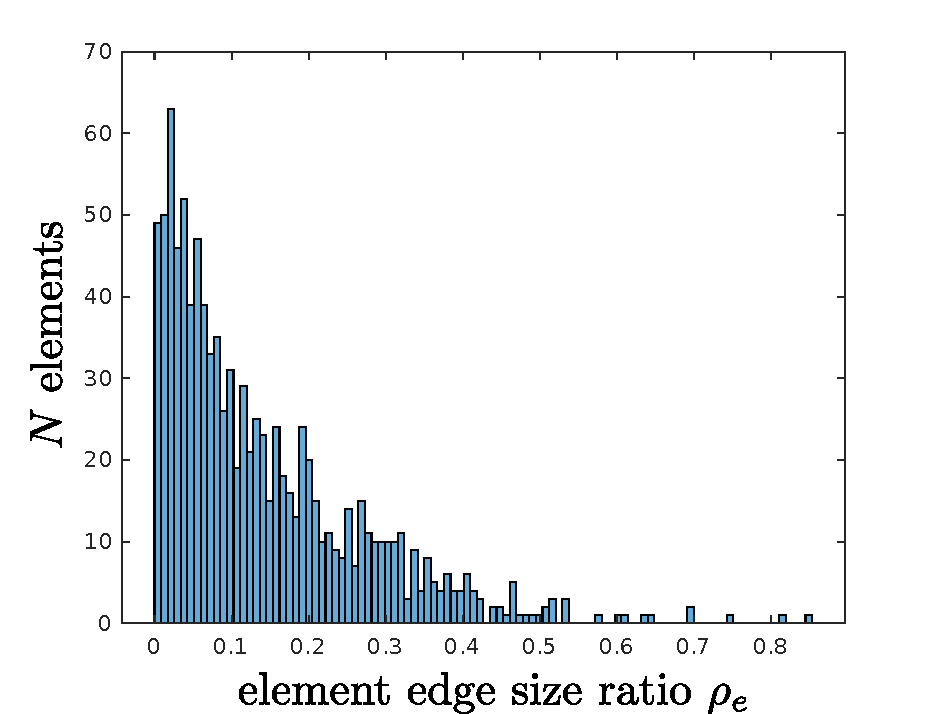
\includegraphics[width=3.0in]{figures/patch_edge_ratios.pdf}
    			\caption{Voronoi mesh \label{fig:patch_edge_ratios}}
    \end{subfigure}
	\begin{subfigure}[b]{0.49\linewidth}
            \centering
            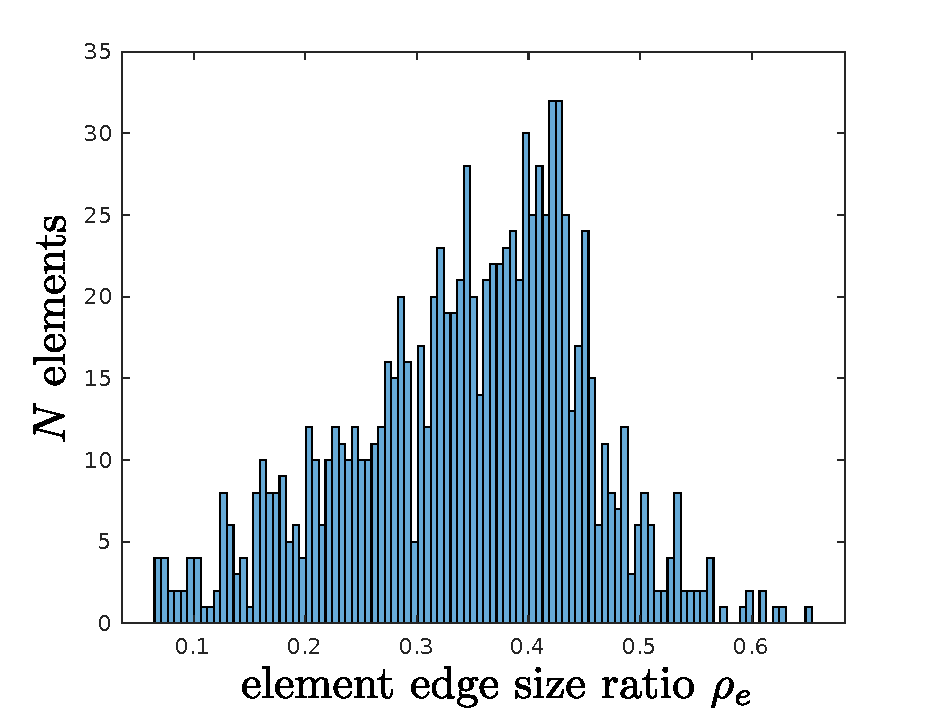
\includegraphics[width=3.0in]{figures/lloyd_edge_ratios.pdf}
    			\caption{Lloyd mesh \label{fig:lloyd_edge_ratios}}
    \end{subfigure}
    \caption{Histograms of various mesh metrics associated with the polygonal meshes depicted in Figure \ref{fig:polygonal_patches}:  (\subref{fig:patch_edge_lengths}) and (\subref{fig:lloyd_edge_lengths}) show the distributions of edge lengths contained in the random Voronoi and Lloyd meshes, respectively; (\subref{fig:patch_edge_ratios}) and (\subref{fig:lloyd_edge_ratios}) show the distributions for the smallest edge length ratios $\rho_e$ in the random Voronoi and Lloyd meshes, respectively.}
\end{figure}

\begin{figure}[!h]
  \centering
  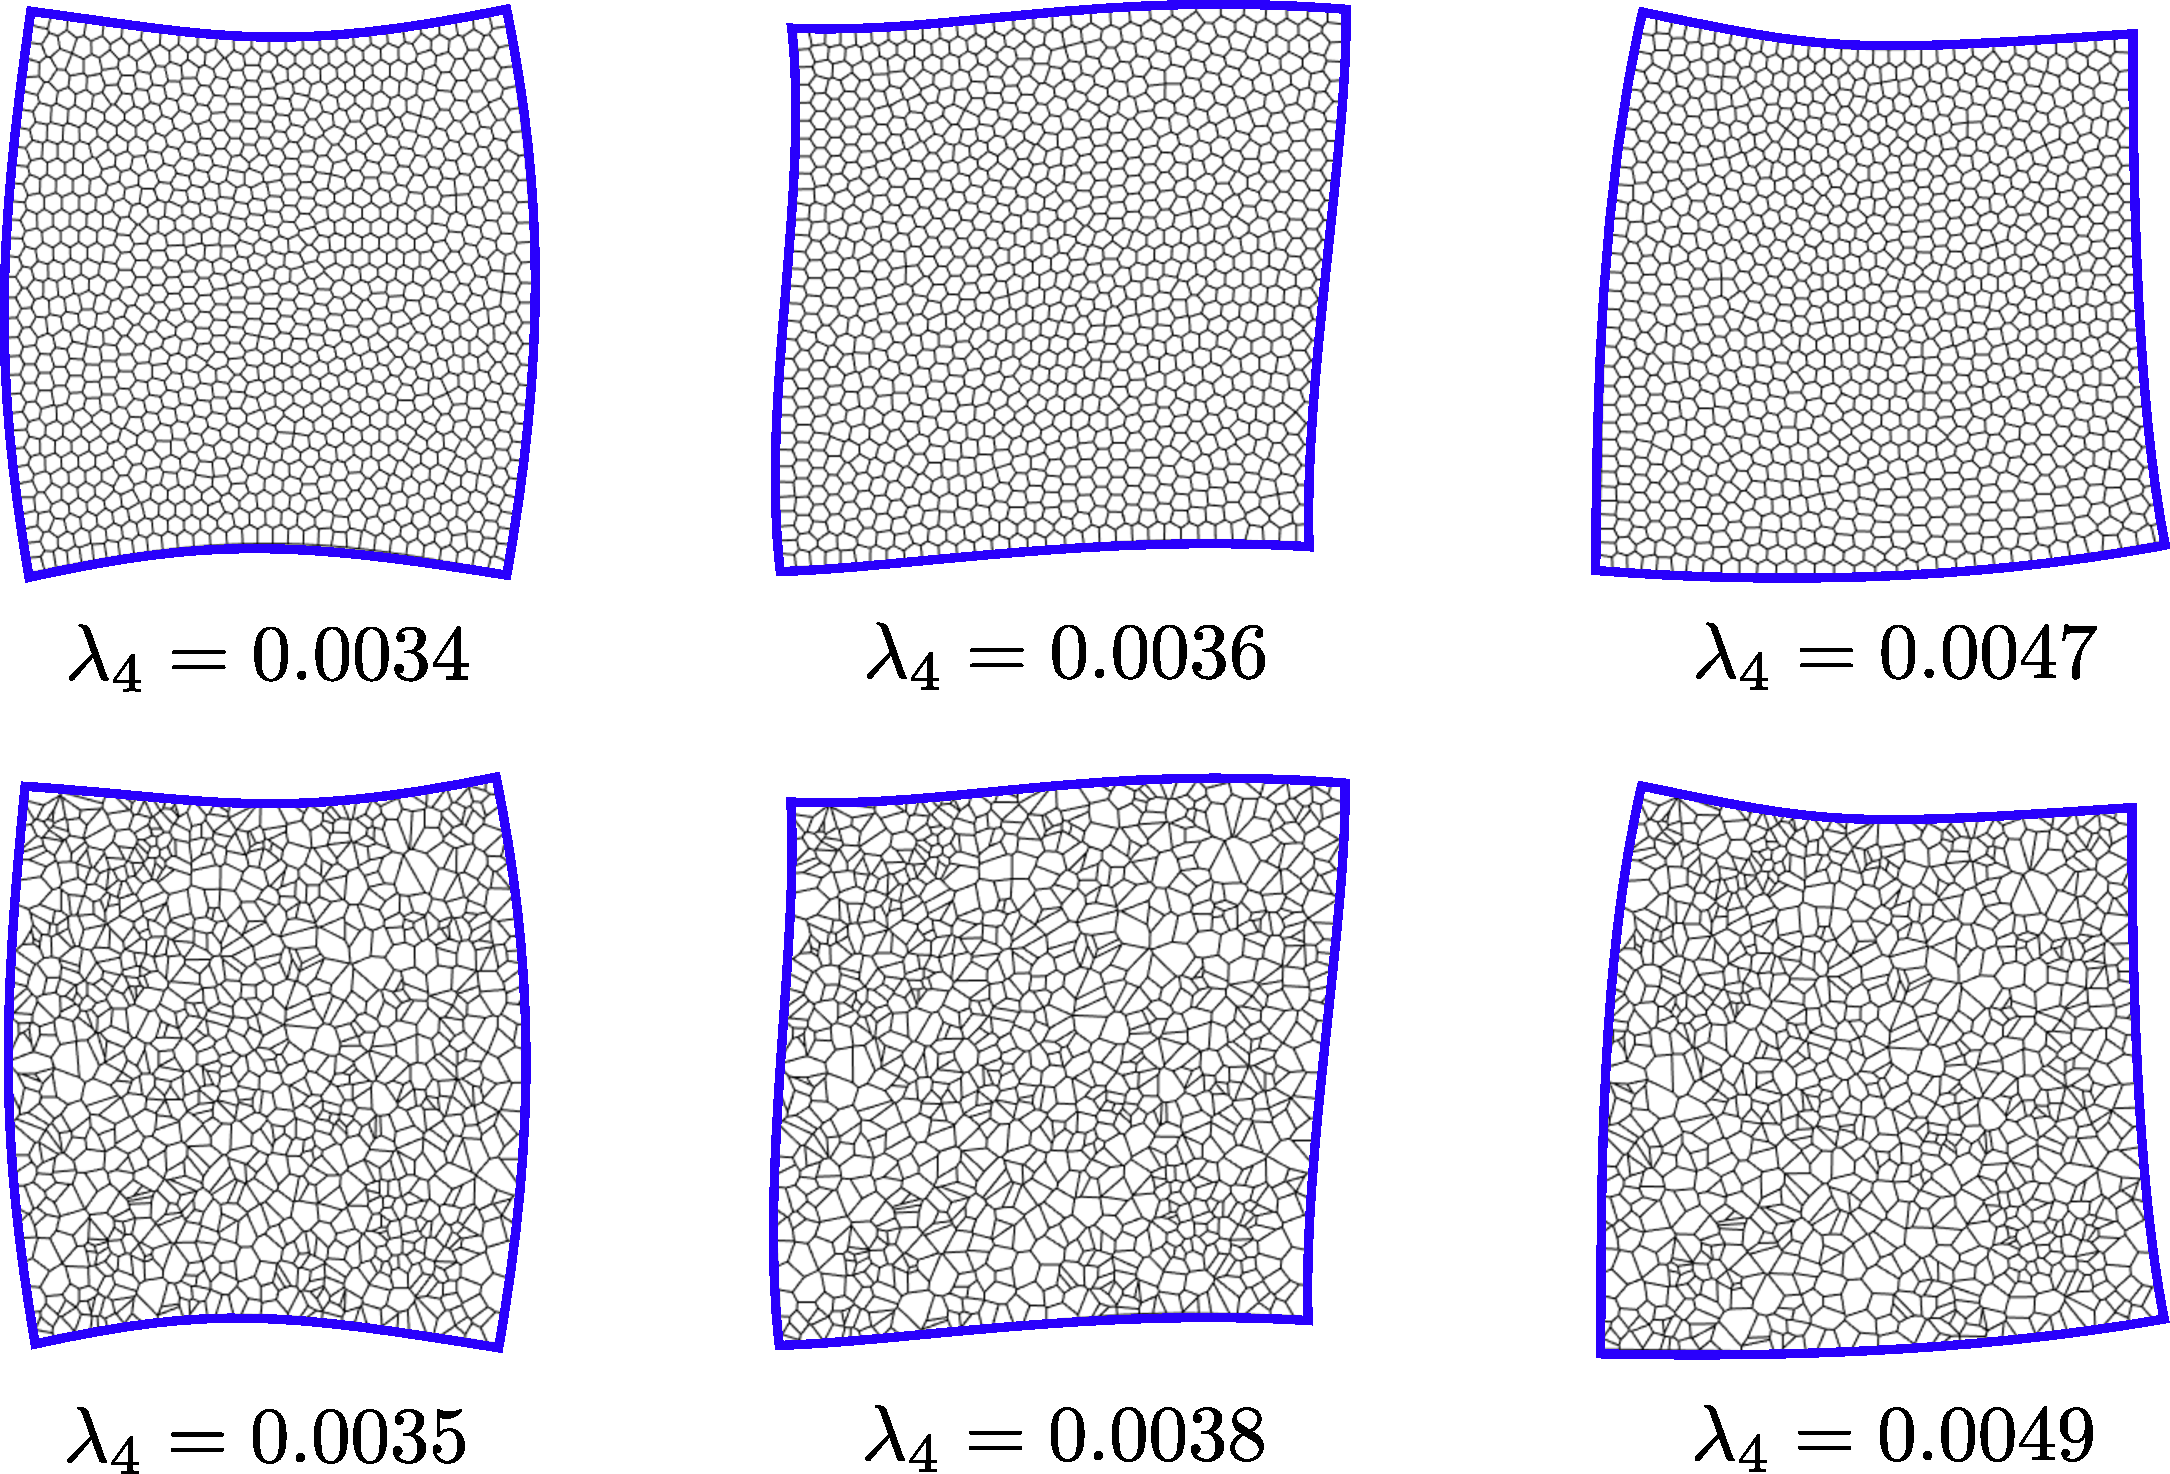
\includegraphics[width=5.0in]{figures/patch_eigenmodes_DGPEM.pdf}  \caption{Depiction of the smallest non-zero eigenvalues and corresponding eigenmodes.}
  \label{fig:patch_eigenmodes_DGPEM}
\end{figure}

\begin{table}[!ht]
  \begin{center}
    \begin{tabular}{| c | c | c |}
    \hline
           & Voronoi mesh & Lloyd mesh \\ \hline
    FE-PEM & 9.1e+05 & 4.6e+03 \\ \hline
    DG-PEM ($\alpha_0 = 10^3$) & 4.8e+04 & 4.4e+03 \\ \hline
    DG-PEM ($\alpha_0 = 10^1$) & 1.0e+03 & 2.9e+03 \\ \hline
    DG-PEM ($\alpha_0 = 10^{-1}$) & 8.1e+02 & 2.7e+03 \\
    \hline
    \end{tabular}
    \caption{Computed values for the condition number $\kappa(\mathbf{K})$ of the global stiffnes matrix $\mathbf{K}$ (excluding rigid body modes).}
    \vspace{-5pt}
    \label{tab:global_stiffness_condition_number}
    \vspace{-25pt}
  \end{center}
\end{table}

% FEPEM - lloyd
% Max E = 1.6e+1
% Mix E = 3.5e-03
% E Rat = 4.6e+03

% FEPEM - patch
% Max E = 3.0e+03
% Mix E = 3.3e-03
% E Rat = 9.1e+05
% Min Emodes:  0.0034, 0.0036, 0.0047

% DGPEM - lloyd - A0 = 1.0e+3
% Max E = 1.5e+1
% Mix E = 3.5e-03
% E Rat = 4.4e+03
% Min Emodes: 0.0035, 0.0038, 0.0049

% DGPEM - patch - A0 = 1.0e+3
% Max E = 1.6e+02
% Mix E = 3.3e-03
% E Rat = 4.8e+04

% DGPEM - lloyd - A0 = 1.0e+1
% Max E = 3.6e+00
% Mix E = 3.5e-03
% E Rat = 1.0e+03

% DGPEM - patch - A0 = 1.0e+1
% Max E = 9.6e+00
% Mix E = 3.3e-03
% E Rat = 2.9e+03

% DGPEM - lloyd - A0 = 1.0e-1
% Max E = 2.8e+00
% Mix E = 3.5e-03
% E Rat = 8.1e+02

% DGPEM - patch - A0 = 1.0e-1
% Max E = 8.9e+00
% Mix E = 3.3e-03
% E Rat = 2.7e+03

\begin{figure}[!h]
    \centering
    \begin{subfigure}[b]{0.49\linewidth}
            \centering
            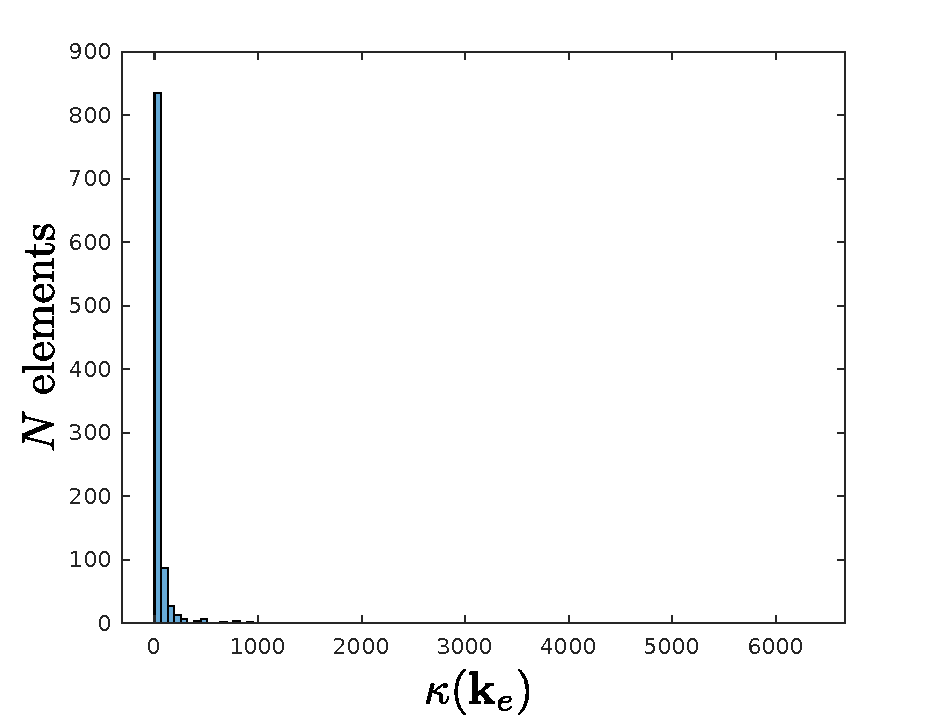
\includegraphics[width=3.0in]{figures/patch_condition_number_FEPEM.pdf}
    			\caption{Voronoi mesh using FE-PEM \label{fig:patch_condition_number_FEPEM}}
    \end{subfigure}
	\begin{subfigure}[b]{0.49\linewidth}
            \centering
            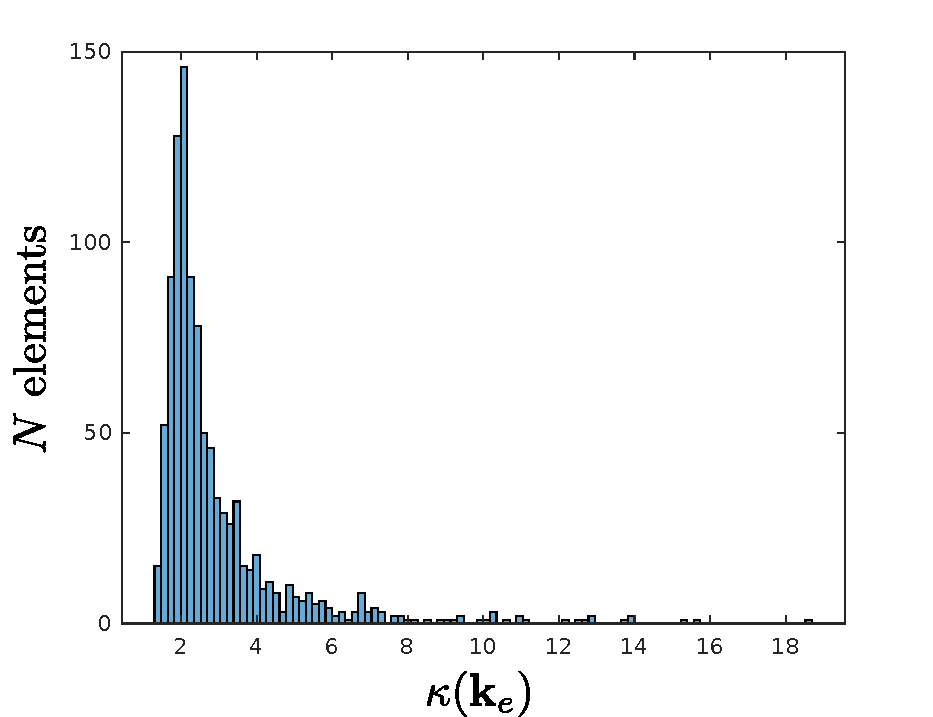
\includegraphics[width=3.0in]{figures/lloyd_condition_number_FEPEM.pdf}
    			\caption{Lloyd mesh using FE-PEM \label{fig:lloyd_condition_number_FEPEM}}
    \end{subfigure}
    \begin{subfigure}[b]{0.49\linewidth}
            \centering
            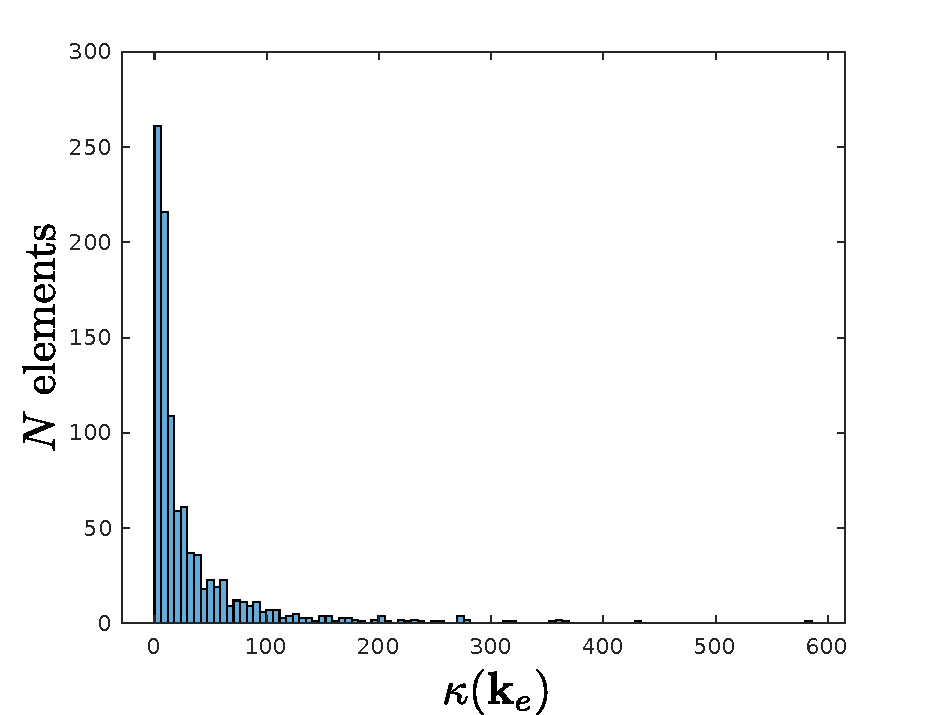
\includegraphics[width=3.0in]{figures/patch_condition_number_DGPEM.pdf}
    			\caption{Voronoi mesh using DG-PEM \label{fig:patch_condition_number_DGPEM}}
    \end{subfigure}
	\begin{subfigure}[b]{0.49\linewidth}
            \centering
            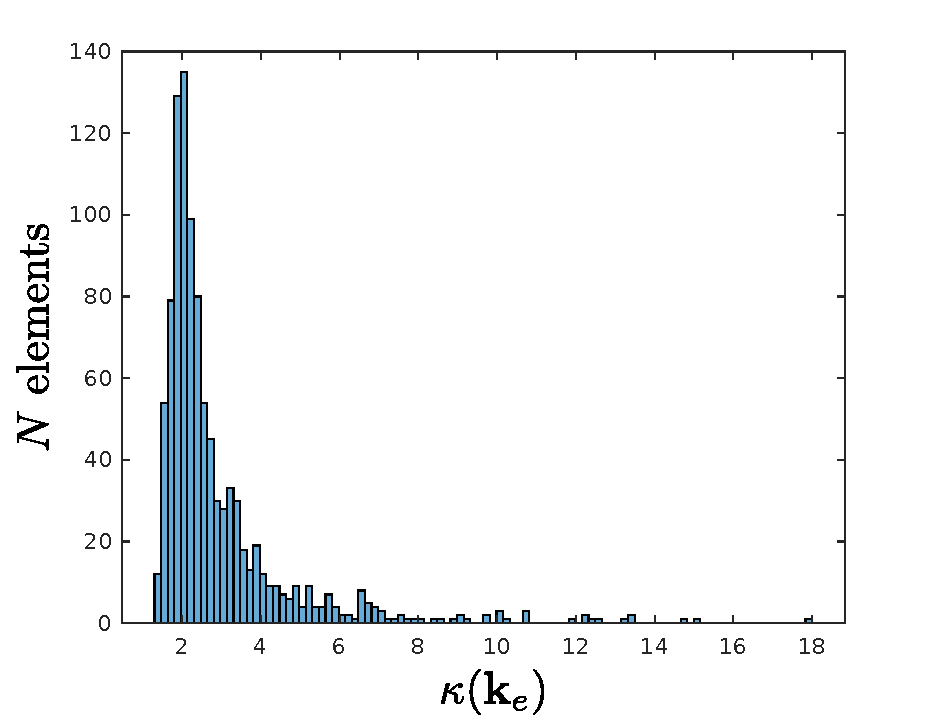
\includegraphics[width=3.0in]{figures/lloyd_condition_number_DGPEM.pdf}
    			\caption{LLoyd mesh using DG-PEM \label{fig:lloyd_condition_number_DGPEM}}
    \end{subfigure}
    \caption{Histograms of various element metrics associated with the polygonal meshes depicted in Figure \ref{fig:polygonal_patches}:  (\subref{fig:patch_edge_lengths}) and (\subref{fig:lloyd_edge_lengths}) show the distributions of edge lengths contained in the random Voronoi and Lloyd meshes, respectively; (\subref{fig:patch_edge_ratios}) and (\subref{fig:lloyd_edge_ratios}) show the distributions for the smallest edge length ratios $\rho_e$ in the random Voronoi and Lloyd meshes, respectively.}
\end{figure}

% local condition number investigation
	% look at DG-PEM system conditioning for certain degenerate elements
	%	* construct a random voronoi mesh on a 2d patch of elements
	%		- get edge-length metrics for voronoi cells
	%   		- examine condition number of local DGPEM systems on these elems
	%       - examine condition number of local stiffness matricies
	%			* look at max and min eigenvalues
	%		- check partition of unity and linear completeness passage
	%		- after grad correction, examine satisfaction of patch tests
	%	* do this for quadratic elements, as well
	%	* do parameter sensitivity analysis
	%	* look at global stiffness matrix condition number
	% look at conditioning for plate-like geometry (anisotropic patch tests)

% check via a series of single-element tests:
	% - examine a test involving a single non-convex element
	%   * shift node around, showing behavior vs. parameterized location
	%     - compare results for VETFEM, DGPEM, and FEPEM vs true harmonic SF
	%     - look at:
	%       * max and min eigenvalues of resulting stiffness matrix
	%       * comment on condition number, and effect on 
	%   * choose different partitioning algorithms / refinement levels
	%   * play around with DGPEM penalization parameters
	%   * examine effects of choosing DG
	% - do a test with a patch of non-convex elements
	%   * examine effects on global stiffness matrix conditioning
	%	* parameterized non-convexity, 

\section{Convergence Analysis}

\subsection*{Infinite Elastic Plate in Far-Field Tension}

\begin{figure}[!h]
  \centering
  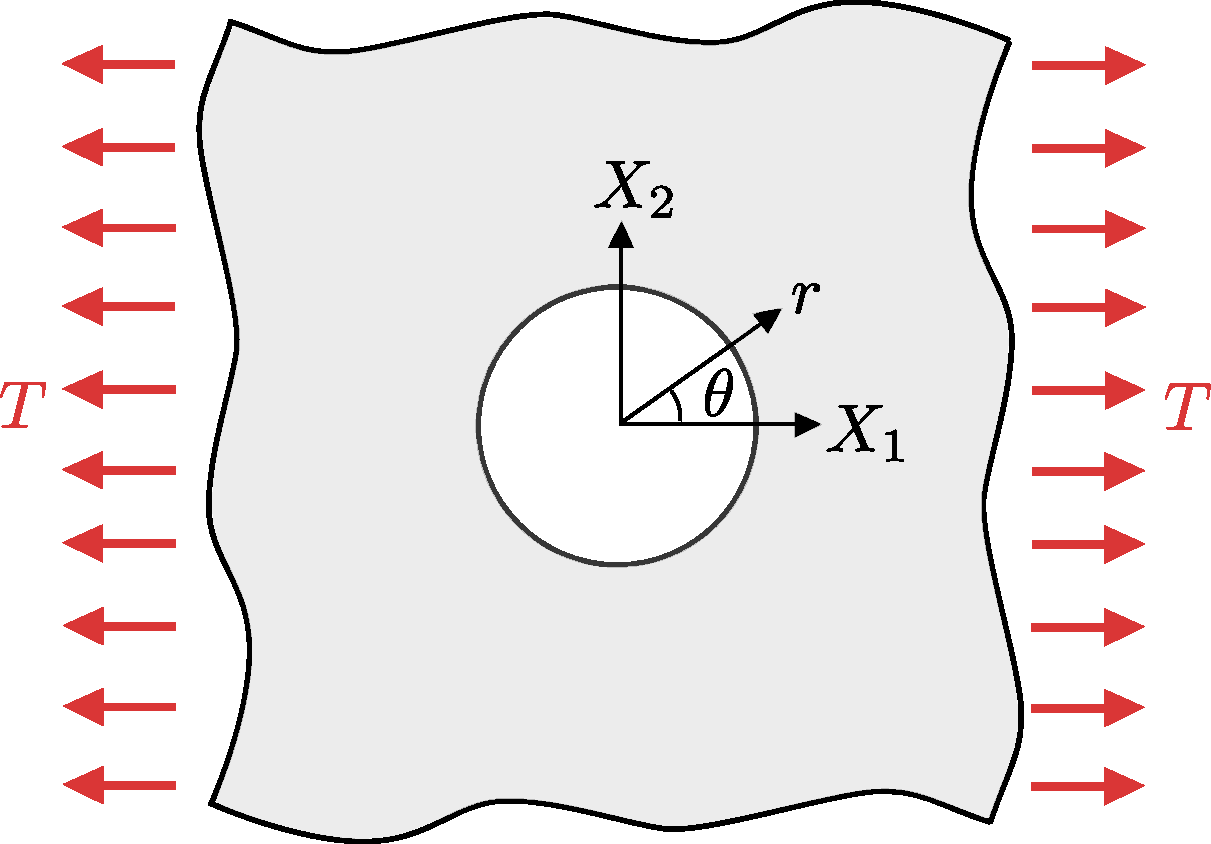
\includegraphics[width=4.0in]{figures/plate_with_hole.pdf}  \caption{Infinite plate with a circular hole placed in uniaxial tension.}
  \label{fig:plate_with_hole_problem}
\end{figure}
To demonstrate optimal convergence of the PEM for higher-order elements, we will choose to investigate the 2D elastostatics problem of an infinite plate with a circular hole in uniaxial tension (depicted in figure \ref{fig:plate_with_hole_problem}), for which there exist analytical solutions of the resulting displacement and stress fields (obtained from reference \cite{Wikiversity:17}):
\begin{equation}
  u_1 (r,\theta) = \frac{Ta}{8\mu} \left[ \frac{r}{a} (\kappa + 1) \cos \theta + \frac{2a}{r} ((1+\kappa) \cos \theta + \cos 3 \theta) - \frac{2a^3}{r^3} \cos 3 \theta \right]
\end{equation}
\begin{equation}
  u_2 (r,\theta) = \frac{Ta}{8\mu} \left[ \frac{r}{a} (\kappa - 3) \sin \theta + \frac{2a}{r} ((1-\kappa) \sin \theta + \sin 3 \theta) - \frac{2a^3}{r^3} \sin 3 \theta \right]
\end{equation}
\begin{equation}
  \sigma_{11} (r, \theta) = T - T \frac{a^2}{r^2} \bigg( \frac{3}{2} \cos 2 \theta + \cos 4 \theta \bigg) + T \frac{3a^4}{2r^4} \cos 4 \theta
\end{equation}
\begin{equation}
  \sigma_{22} (r, \theta) = - T \frac{a^2}{r^2} \bigg( \frac{1}{2} \cos 2 \theta - \cos 4 \theta \bigg) - T \frac{3a^4}{2r^4} \cos 4 \theta
\end{equation}
\begin{equation}
  \sigma_{12} (r, \theta) = - T \frac{a^2}{r^2} \bigg( \frac{1}{2} \sin 2 \theta + \sin 4 \theta \bigg) + T \frac{3a^4}{2r^4} \sin 4 \theta
\end{equation}
where $T$ is the far-field value of the applied tensile stress, $a$ is the radius of the circular hole centered at $r=0$, $\kappa = 4 - 3\nu$ (under plane-strain conditions), and $\nu$ and $\mu$ are the the Poisson's ratio and shear modulus of the material, respectively.

\begin{figure}[!h]
  \centering
  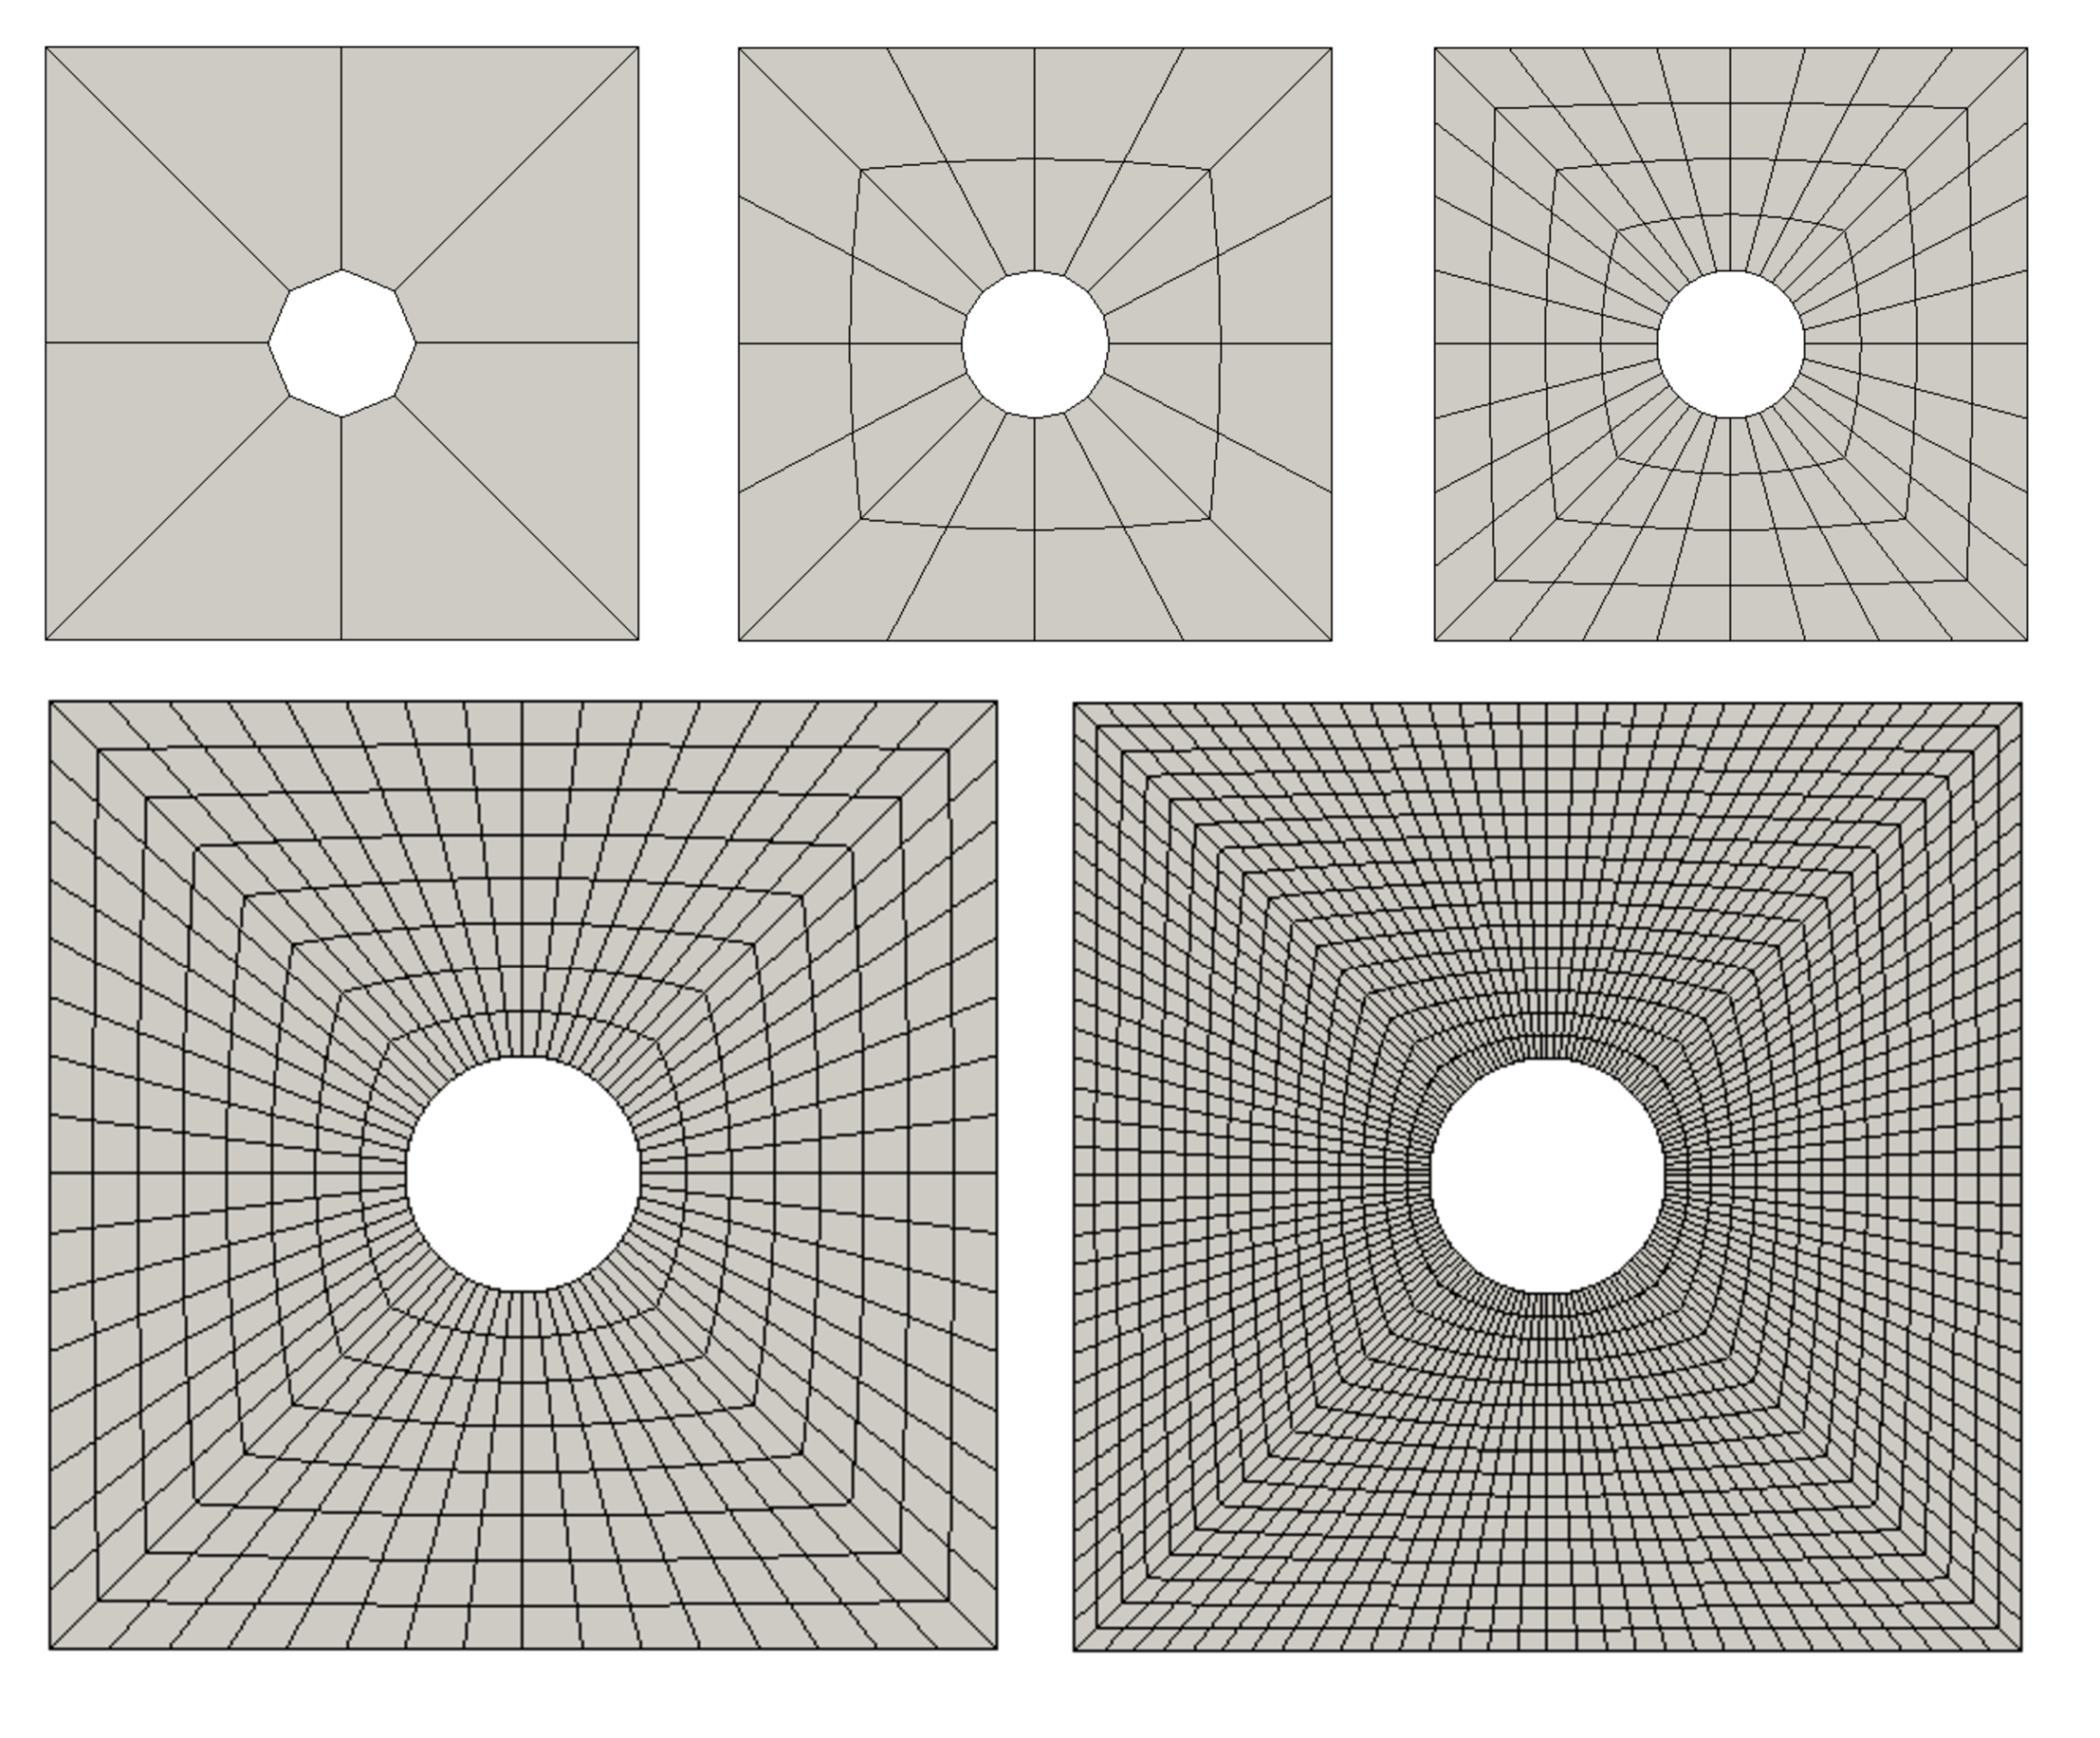
\includegraphics[width=6.0in]{figures/plate_with_hole_meshes.pdf}
  \caption{Quadrilateral meshes with varying levels of refinement.}
  \label{fig:plate_with_hole_meshes}
\end{figure}
A convergence study was carried out using a series of quadrilateral meshes with varying levels of refinement discretizing the restricted problem domain $X_i \in [ -1, +1]$ (see figure \ref{fig:plate_with_hole_meshes}.) The meshes consisted of either 4-node quadrilateral or 8-node serendipity quadrilateral elements, and employed either an isoparametric formulation, or a sufficiently high-order PEM formulation (i.e. $k=1$ for 4-node quadrilaterals, and $k=2$ for 8-node quadrilaterals.) Displacement boundary conditions were prescribed to be consistent with the exact solution on the restricted boundary. $L^2$ displacement error norms and $H^1$ energy error semi-norms were computed with reference to the exact solution, with the numerical results summarized in tables \ref{tab:l2_error}-\ref{tab:h1_rates}. The convergence rates in the $L^2$ and $H^1$ error norms are depicted in figures \ref{fig:l2_error} and \ref{fig:h1_error}, respectively.
\newpage
\begin{table}[!ht]
  \begin{center}
    \begin{tabular}{| c | c | c | c | c |}
    \hline
    $h$ & 4-node FEM & 4-node PEM & 8-node FEM & 8-node PEM \\ \hline
    1.2500 & 1.3133E-006 & 1.4901E-006 & 9.8369E-007 & 2.9990E-006 \\ \hline
    0.8006 & 6.9557E-007 & 9.8453E-007 & 4.8165E-007 & 1.3918E-006 \\ \hline
    0.4488 & 2.8755E-007 & 4.2859E-007 & 2.2034E-007 & 3.3673E-007 \\ \hline
    0.2371 & 1.0460E-007 & 1.3672E-007 & 8.1971E-008 & 4.8942E-008 \\ \hline
    0.1218 & 3.1430E-008 & 3.7296E-008 & 2.4628E-008 & 6.7201E-009 \\ \hline
    0.0617 & 8.3877E-009 & 9.5661E-009 & 6.5479E-009 & 1.6002E-009 \\
    \hline
    \end{tabular}
    \caption{Computed $L^2$ displacement error norms.}
    \vspace{-5pt}
    \label{tab:l2_error}
    \vspace{-25pt}
  \end{center}
\end{table}
\begin{table}[!ht]
  \begin{center}
    \begin{tabular}{| c | c | c | c | c |}
    \hline
    $h$ & 4-node FEM & 4-node PEM & 8-node FEM & 8-node PEM \\ \hline
    1.2500 &	-	&	-	&	-	&       -      \\ \hline
    0.8006 &	1.4265	&	0.9302	&	1.6028	&	1.7230 \\ \hline
    0.4488 &	1.5262	&	1.4369	&	1.3512	&	2.4518 \\ \hline
    0.2371 &	1.5848	&	1.7906	&	1.5496	&	3.0225 \\ \hline
    0.1218 &	1.8051	&	1.9502	&	1.8053	&	2.9808 \\ \hline
    0.0617 &	1.9424	&	2.0007	&	1.9479	&	2.1100 \\
    \hline
    \end{tabular}
    \caption{Computed $L^2$ displacement error norm convergence rates.}
    \vspace{-5pt}
    \label{tab:l2_rates}
    \vspace{-25pt}
  \end{center}
\end{table}
\begin{table}[!ht]
  \begin{center}
    \begin{tabular}{| c | c | c | c | c |}
    \hline
    $h$ & 4-node FEM & 4-node PEM & 8-node FEM & 8-node PEM \\ \hline
    1.2500 & 2.1468E-001 & 2.8913E-001 & 1.8275E-001 & 5.3700E-001 \\ \hline
    0.8006 & 1.8622E-001 & 2.5620E-001 & 1.5959E-001 & 3.0529E-001 \\ \hline
    0.4488 & 1.3786E-001 & 1.7930E-001 & 1.2495E-001 & 1.5310E-001 \\ \hline
    0.2371 & 9.2075E-002 & 1.1251E-001 & 7.9144E-002 & 5.8671E-002 \\ \hline
    0.1218 & 5.2124E-002 & 6.2223E-002 & 4.2868E-002 & 1.5541E-002 \\ \hline
    0.0617 & 2.7048E-002 & 3.2135E-002 & 2.1789E-002 & 3.3672E-003 \\
    \hline
    \end{tabular}
    \caption{Computed $H^1$ energy error semi-norms.}
    \vspace{-5pt}
    \label{tab:h1_error}
    \vspace{-25pt}
  \end{center}
\end{table}
\begin{table}[!ht]
  \begin{center}
    \begin{tabular}{| c | c | c | c | c |}
    \hline
    $h$ & 4-node FEM & 4-node PEM & 8-node FEM & 8-node PEM \\ \hline
    1.2500 &	-	&	-	&	-	&       -      \\ \hline
    0.8006 &	0.3192	&	0.2714	&	0.3042	&	1.2675 \\ \hline
    0.4488 &	0.5195	&	0.6166	&	0.4228	&	1.1924 \\ \hline
    0.2371 &	0.6326	&	0.7303	&	0.7156	&	1.5031 \\ \hline
    0.1218 &	0.8542	&	0.8892	&	0.9205	&	1.9944 \\ \hline
    0.0617 &	0.9646	&	0.9716	&	0.9950	&	2.2488 \\
    \hline
    \end{tabular}
    \caption{Computed $H^1$ energy error semi-norm convergence rates.}
    \vspace{-5pt}
    \label{tab:h1_rates}
    \vspace{-25pt}
  \end{center}
\end{table}
\begin{figure}[!h]
  \centering
  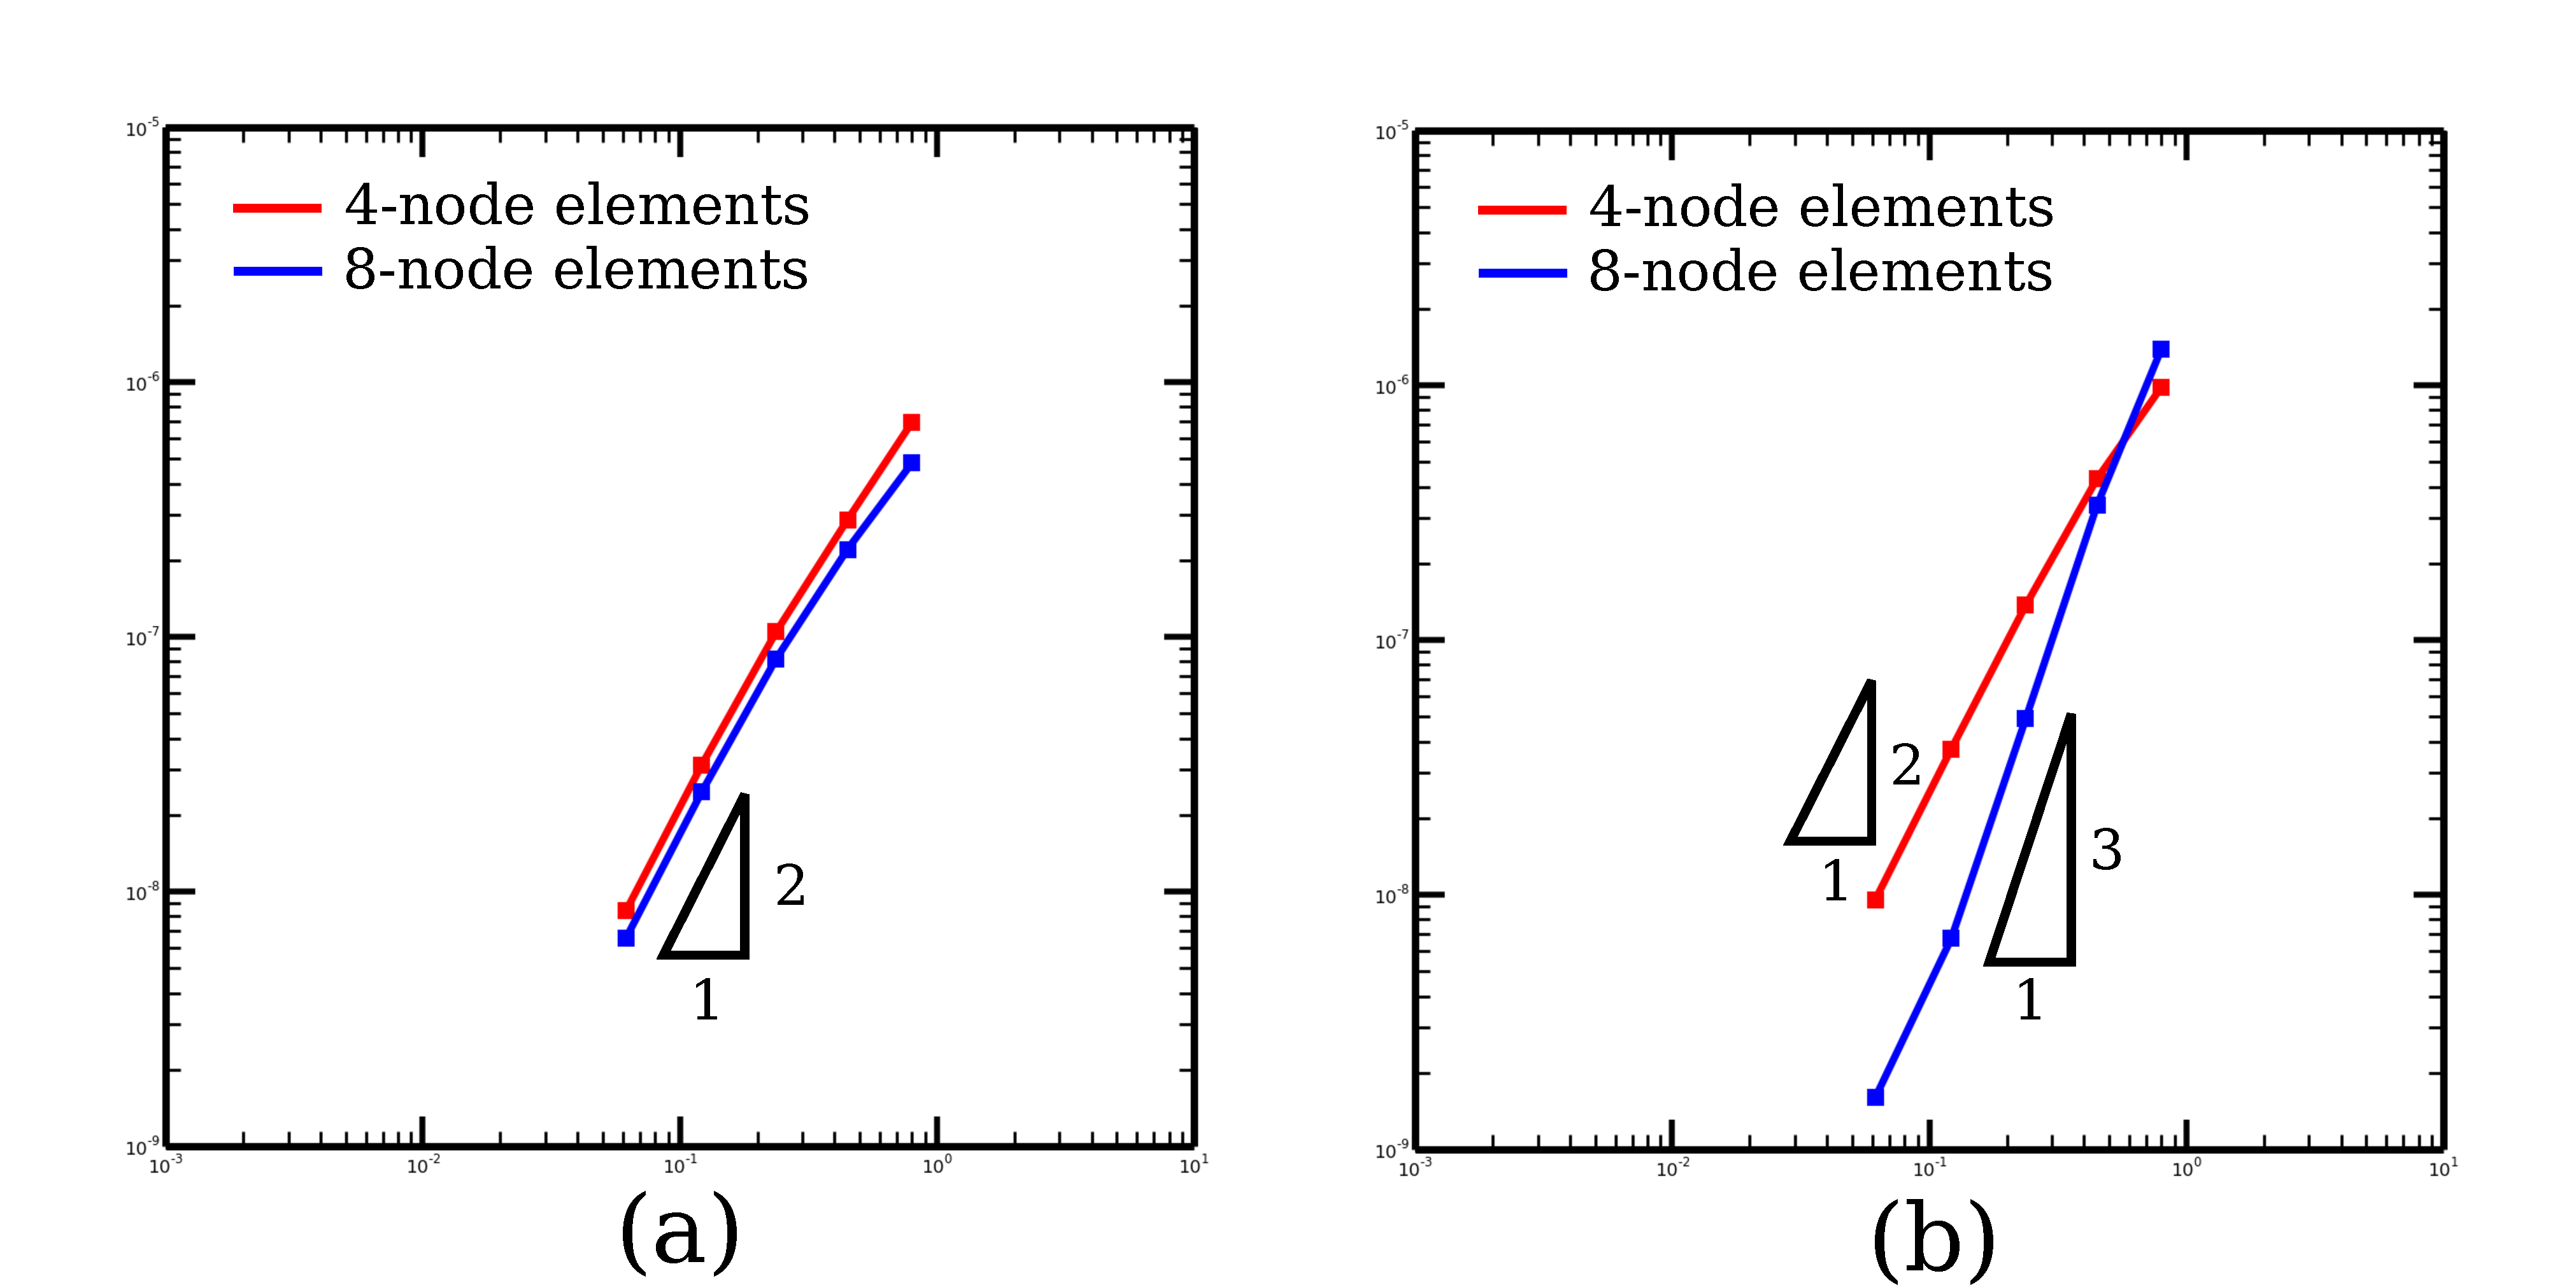
\includegraphics[width=6.0in]{figures/l2_error_plot.pdf}
  \caption{$L^2$ error convergence plots for (a) FEM and (b) PEM formulations.}
  \label{fig:l2_error}
  \vspace{-10pt}
\end{figure}

\begin{figure}[!h]
  \centering
  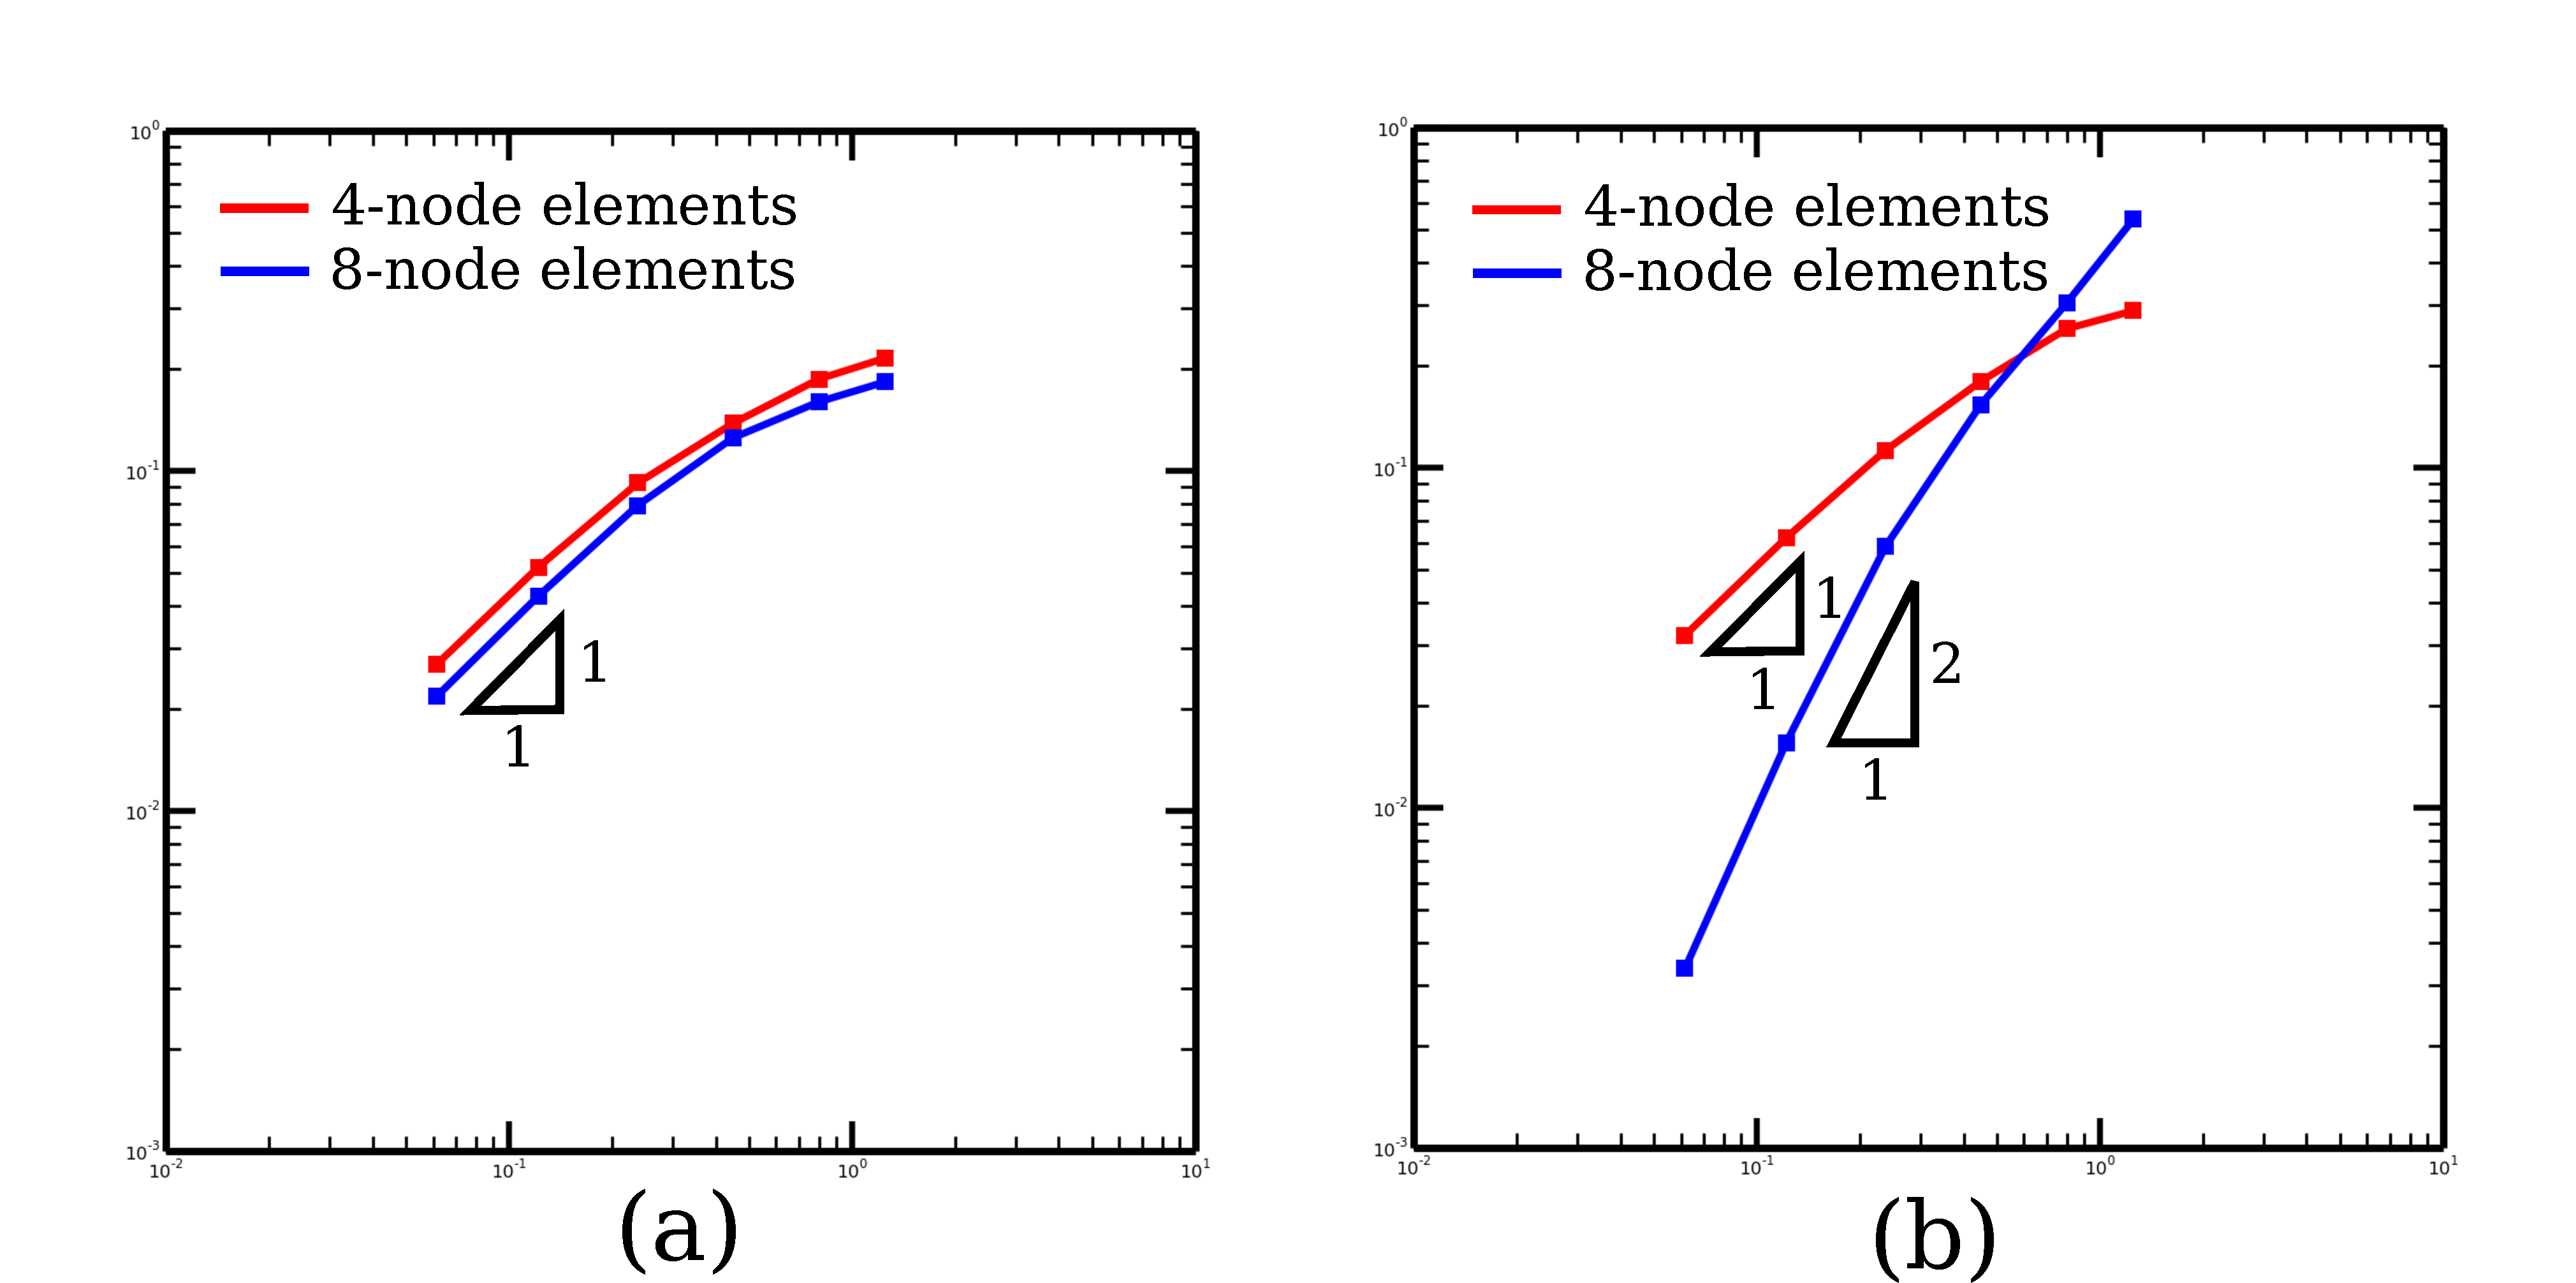
\includegraphics[width=6.0in]{figures/h1_error_plot.pdf}
  \caption{$H^1$ error convergence plots for (a) FEM and (b) PEM formulations.}
  \label{fig:h1_error}
\end{figure}

A number of observations should be made regarding the resulting data. In particular, it is worthwhile to note that part of the incurred solution error may be attributable to the inexact representation of the problem geometry, especially for the coarse meshes. This may in part explain why the observed convergence rates are lower at coarser levels of refinement, but approach the expected rates as the mesh is further refined.

Additionally, we remark that isoparametric serendipity quadrilateral elements converge at sub-optimal rates if the elements are distorted in a non-affine fashion (as is the case for our meshes). This is an altogether expected result, and has been discussed in references \cite{Arnold:01} and \cite{Arnold:02}.

Conversely, we observe that the PEM quadrilateral elements converge at the optimal rates in both the $L^2$ and $H^1$ error norms, as we would hope.

Further work will seek to investigate the measured error and convergence rates of the PEM when the elements take on arbitrary shape, and for a variety of different formulations and penalization parameter settings.

\section{Parameter Sensitivity Analysis}

\section{Computational Efficiency}
\subsection{Performance Comparison}

\section{Resistance to Locking Phenomena}

\subsection*{Twisting Annulus}

Consider an incompressible elastic annulus whose inner radius at $r = R_i$ is fixed, and whose outer radius $r = R_o$ rigidly rotates at an angular velocity of $\Phi$. The radially symmetric displacement boundary conditions for this motion are described by
\begin{equation}
	u_r (R_i,t) = u_r (R_o,t) = 0, \quad u_z (R_i,t) = u_z (R_o,t) = 0,
\end{equation}
\begin{equation}
	u_\theta (R_i,t) = 0, \quad u_\theta (R_o,t) = R_o \, \Phi \, t,
\end{equation}
for all $t \geq 0$.

The elastic material is characterized by a linear hypoelastic material model of grade zero, obeying
\begin{equation}
  \dot{\boldsymbol{\sigma}} = \mathbb{C} : \mathbf{D} + \mathbf{W} \boldsymbol{\sigma} - \boldsymbol{\sigma} \mathbf{W},
\end{equation}

\subsubsection*{Exact Solution}

An exact solution for the aforementioned problem may be obtained by considering the stress divergence equations in cylindrical polar coordinates:
\begin{equation}
  \nabla \cdot \boldsymbol{\sigma} = \left\{ \begin{array}{c} \frac{\partial \sigma_{rr}}{\partial r} + \frac{\sigma_{rr}}{r} + \frac{1}{r} \frac{\partial \sigma_{\theta r}}{\partial \theta} + \frac{\partial \sigma_{z r}}{\partial z} - \frac{\sigma_{\theta \theta}}{r} \\
    \frac{1}{r} \frac{\partial \sigma_{\theta \theta}}{\partial \theta} + \frac{\partial \sigma_{r\theta}}{\partial r} + \frac{\sigma_{r\theta}}{r} + \frac{\sigma_{\theta r}}{r} + \frac{\partial \sigma_{z \theta}}{\partial z} \\
    \frac{\partial \sigma_{z z}}{\partial z} + \frac{\partial \sigma_{r z}}{\partial r} + \frac{\sigma_{r z}}{r} + \frac{1}{r} \frac{\partial \sigma_{\theta z}}{\partial \theta} \end{array} \right\} = \mathbf{0}.
\end{equation}
By the assumptions of plane strain and axisymmetry, we rationalize that $\boldsymbol{\sigma} (r)$ is a function of $r$, alone, and therefore,
\begin{equation}
  \nabla \cdot \boldsymbol{\sigma} = \left\{ \begin{array}{c} \frac{\partial \sigma_{rr}}{\partial r} + \frac{\sigma_{rr} - \sigma_{\theta \theta}}{r} \\
    \frac{\partial \sigma_{r\theta}}{\partial r} + \frac{2 \sigma_{r\theta}}{r} \\
    \frac{\partial \sigma_{r z}}{\partial r} + \frac{\sigma_{r z}}{r} \end{array} \right\} = \mathbf{0}.
\end{equation}
Furthermore, by the assumptions of plane strain, we observe that $\sigma_{rz} = 0$ and $\sigma_{\theta z} = 0$. Additionally, if we impose the incompressibility condition $\nabla \cdot \mathbf{v} = \text{tr} (\mathbf{D}) = 0$, we find that
\begin{equation}
  \text{tr} (\dot{\boldsymbol{\sigma}}) = 0 \, \Rightarrow \, \text{tr} (\boldsymbol{\sigma}) = 0 \, \forall t.
\end{equation}
The deformation necessitates that $\sigma_{zz} = 0$, and therefore $\sigma_{\theta \theta} = - \sigma_{rr}$. Consequently, we are left with 2 governing differential equations for $\sigma_{rr}$ and $\sigma_{r \theta}$:
\begin{equation}
  \frac{\partial \sigma_{rr}}{\partial r} + \frac{2 \sigma_{rr}}{r} = 0, \quad \frac{\partial \sigma_{r\theta}}{\partial r} + \frac{2 \sigma_{r\theta}}{r} = 0,
\end{equation}
whose solutions are of the form
\begin{equation}
  \sigma_{rr} = \frac{a}{r^2}, \quad \sigma_{r\theta} = \frac{b}{r^2}.
\end{equation}
Consequently,
\begin{equation}
  \left\{ \begin{array}{c} \sigma_{rr} \\ \sigma_{\theta \theta} \\ \sigma_{r \theta} \end{array} \right\} = r^{-2} \left\{ \begin{array}{c} +a \\ -a \\ b \end{array} \right\}.
\end{equation}

Under the assumption of incompressibility, we may characterize the deformation via the velocity field $v_r = 0$, $v_z = 0$, and $v_\theta (r) = r \dot{\phi}(r)$, yielding the velocity gradient (in cylindrical polar coordinates):
\begin{equation}
  \mathbf{L} = \nabla \mathbf{v} = \left[ \begin{array}{ccc} v_{r,r} & v_{r,\theta}/r-v_\theta /r & v_{r,z} \\
      v_{\theta,r} & v_{\theta,\theta}/r + v_r /r & v_{\theta,z} \\
      v_{z,r} & v_{z,\theta} /r & v_{z,z} \end{array} \right] = 
  \left[ \begin{array}{ccc} 0 & -\dot{\phi} & 0 \\
      \dot{\phi} + r \dot{\phi}_{,r} & 0 & 0 \\
      0 & 0 & 0 \end{array} \right],
\end{equation}
and the corresponding rate of deformation and spin tensors:
\begin{equation}
  \mathbf{D} = \frac{r \dot{\phi}_{,r}}{2} \left[ \begin{array}{ccc} 0 & 1 & 0 \\
      1 & 0 & 0 \\
      0 & 0 & 0 \end{array} \right], \quad \mathbf{W} = 
  \frac{2 \dot{\phi} + r \dot{\phi}_{,r}}{2} \left[ \begin{array}{ccc} 0 & - 1 & 0 \\
      1 & 0 & 0 \\
      0 & 0 & 0 \end{array} \right].
\end{equation}
The resulting stress rate equations are
\begin{equation}
  \left\{ \begin{array}{c} \dot{\sigma}_{rr} \\ \dot{\sigma}_{\theta \theta} \\ \dot{\sigma}_{r \theta} \end{array} \right\} = \left\{ \begin{array}{c} 0 \\ 0 \\ \mu r \dot{\phi}_{,r} \end{array} \right\} + 
  (2 \dot{\phi} + r \dot{\phi}_{,r}) \left\{ \begin{array}{c} - \sigma_{r \theta} \\ \sigma_{r \theta} \\ \sigma_{rr} \end{array} \right\},
\end{equation}
or
\begin{equation}
  \left\{ \begin{array}{c} \dot{a} \\ \dot{b} \end{array} \right\} = \left\{ \begin{array}{c} 0 \\ \mu r^3 \dot{\phi}_{,r} \end{array} \right\} + (2 \dot{\phi} + r \dot{\phi}_{,r}) \left[ \begin{array}{cc} 0 & -1 \\ 1 & 0 \end{array} \right] \left\{ \begin{array}{c} a \\ b \end{array} \right\},
\end{equation}
which must be valid $\forall r, \, t$. If we assume that $\dot{\phi} = f(r)$ is a function of $r$ (and not of $t$), then we obtain the condition
\begin{equation}
  3 f_{,r} + r f_{,rr} = 0,
\end{equation}
implying $f_{,r} = B r^{-3}$, and $\phi (r, t) = (A - B r^{-2} / 2)t$, thus
\begin{equation}
  \left\{ \begin{array}{c} \dot{a} \\ \dot{b} \end{array} \right\} = \left\{ \begin{array}{c} 0 \\ \mu B \end{array} \right\} + 2 A \left[ \begin{array}{cc} 0 & -1 \\ 1 & 0 \end{array} \right] \left\{ \begin{array}{c} a \\ b \end{array} \right\},
\end{equation}
and
\begin{equation}
  a(t) = - \frac{\mu B}{2 A} - C_2 \sin (2 A t) + C_1 \cos (2 A t),
\end{equation}
\begin{equation}
  b(t) = C_1 \sin (2 A t) + C_2 \cos (2 A t).
\end{equation}
Imposing the initial conditions $a(0) = b(0) = 0$ results in:
\begin{equation}
  a(t) = \frac{\mu B}{2 A} \left[ \cos (2 A t) - 1 \right], \quad b(t) = \frac{\mu B}{2 A} \sin (2 A t).
\end{equation}
Imposing the boundary conditions $\phi(R_i,t) = 0 \, \, \forall t$, $\phi(R_o,t) = \Phi \, t \, \, \forall t$ yields:
\begin{equation}
  A = \frac{\Phi R_i^{-2}}{R_i^{-2} - R_o^{-2}}, \quad B = \frac{2 \Phi}{R_i^{-2} - R_o^{-2}}.
\end{equation}

The final analytical solution for the displacement and stress fields is presented below:
\begin{equation}
  u_r = 0, \quad u_\theta = r \Phi \frac{R_i^{-2} - r^{-2}}{R_i^{-2} - R_o^{-2}} t, \quad u_z = 0,
\end{equation}
\begin{equation}
  \sigma_{rr} = - \sigma_{\theta \theta} = \mu \frac{r^{-2}}{R_i^{-2}} \left[ \cos \left( 2 \frac{\Phi R_i^{-2}}{R_i^{-2} - R_o^{-2}} t \right) - 1 \right],
\end{equation}
\begin{equation}
  \sigma_{r \theta} = \mu \frac{r^{-2}}{R_i^{-2}} \sin \left( 2 \frac{\Phi R_i^{-2}}{R_i^{-2} - R_o^{-2}} t \right).
\end{equation}

\subsubsection*{Numerical Results}

Because the element formulations that will be used herein possess only displacement degrees of freedom, we expect the finite element solutions to present innaccuracies due to the effects of volumetric locking. Moreover, it is not possible to run an analysis for a truly incompressible material (if the grade zero hypoelasticity model is to be utilized). For this reasons, it will suffice to examine solutions in the near-incompressible regieme (i.e. $\nu = 0.4999$).

Additionally, because an accurate prediction of the pressure field requires the use of a mixed formulation, we expect the stress error to be dominated by errors in the pressure field. For this reason, we will choose to examine only the errors in the deviatoric stress field, where $s_{ij} = \sigma_{ij} - \frac{1}{3} \delta_{ij} \sigma_{kk}$ denotes the stress deviator.

\begin{figure}[!h]
  \centering
  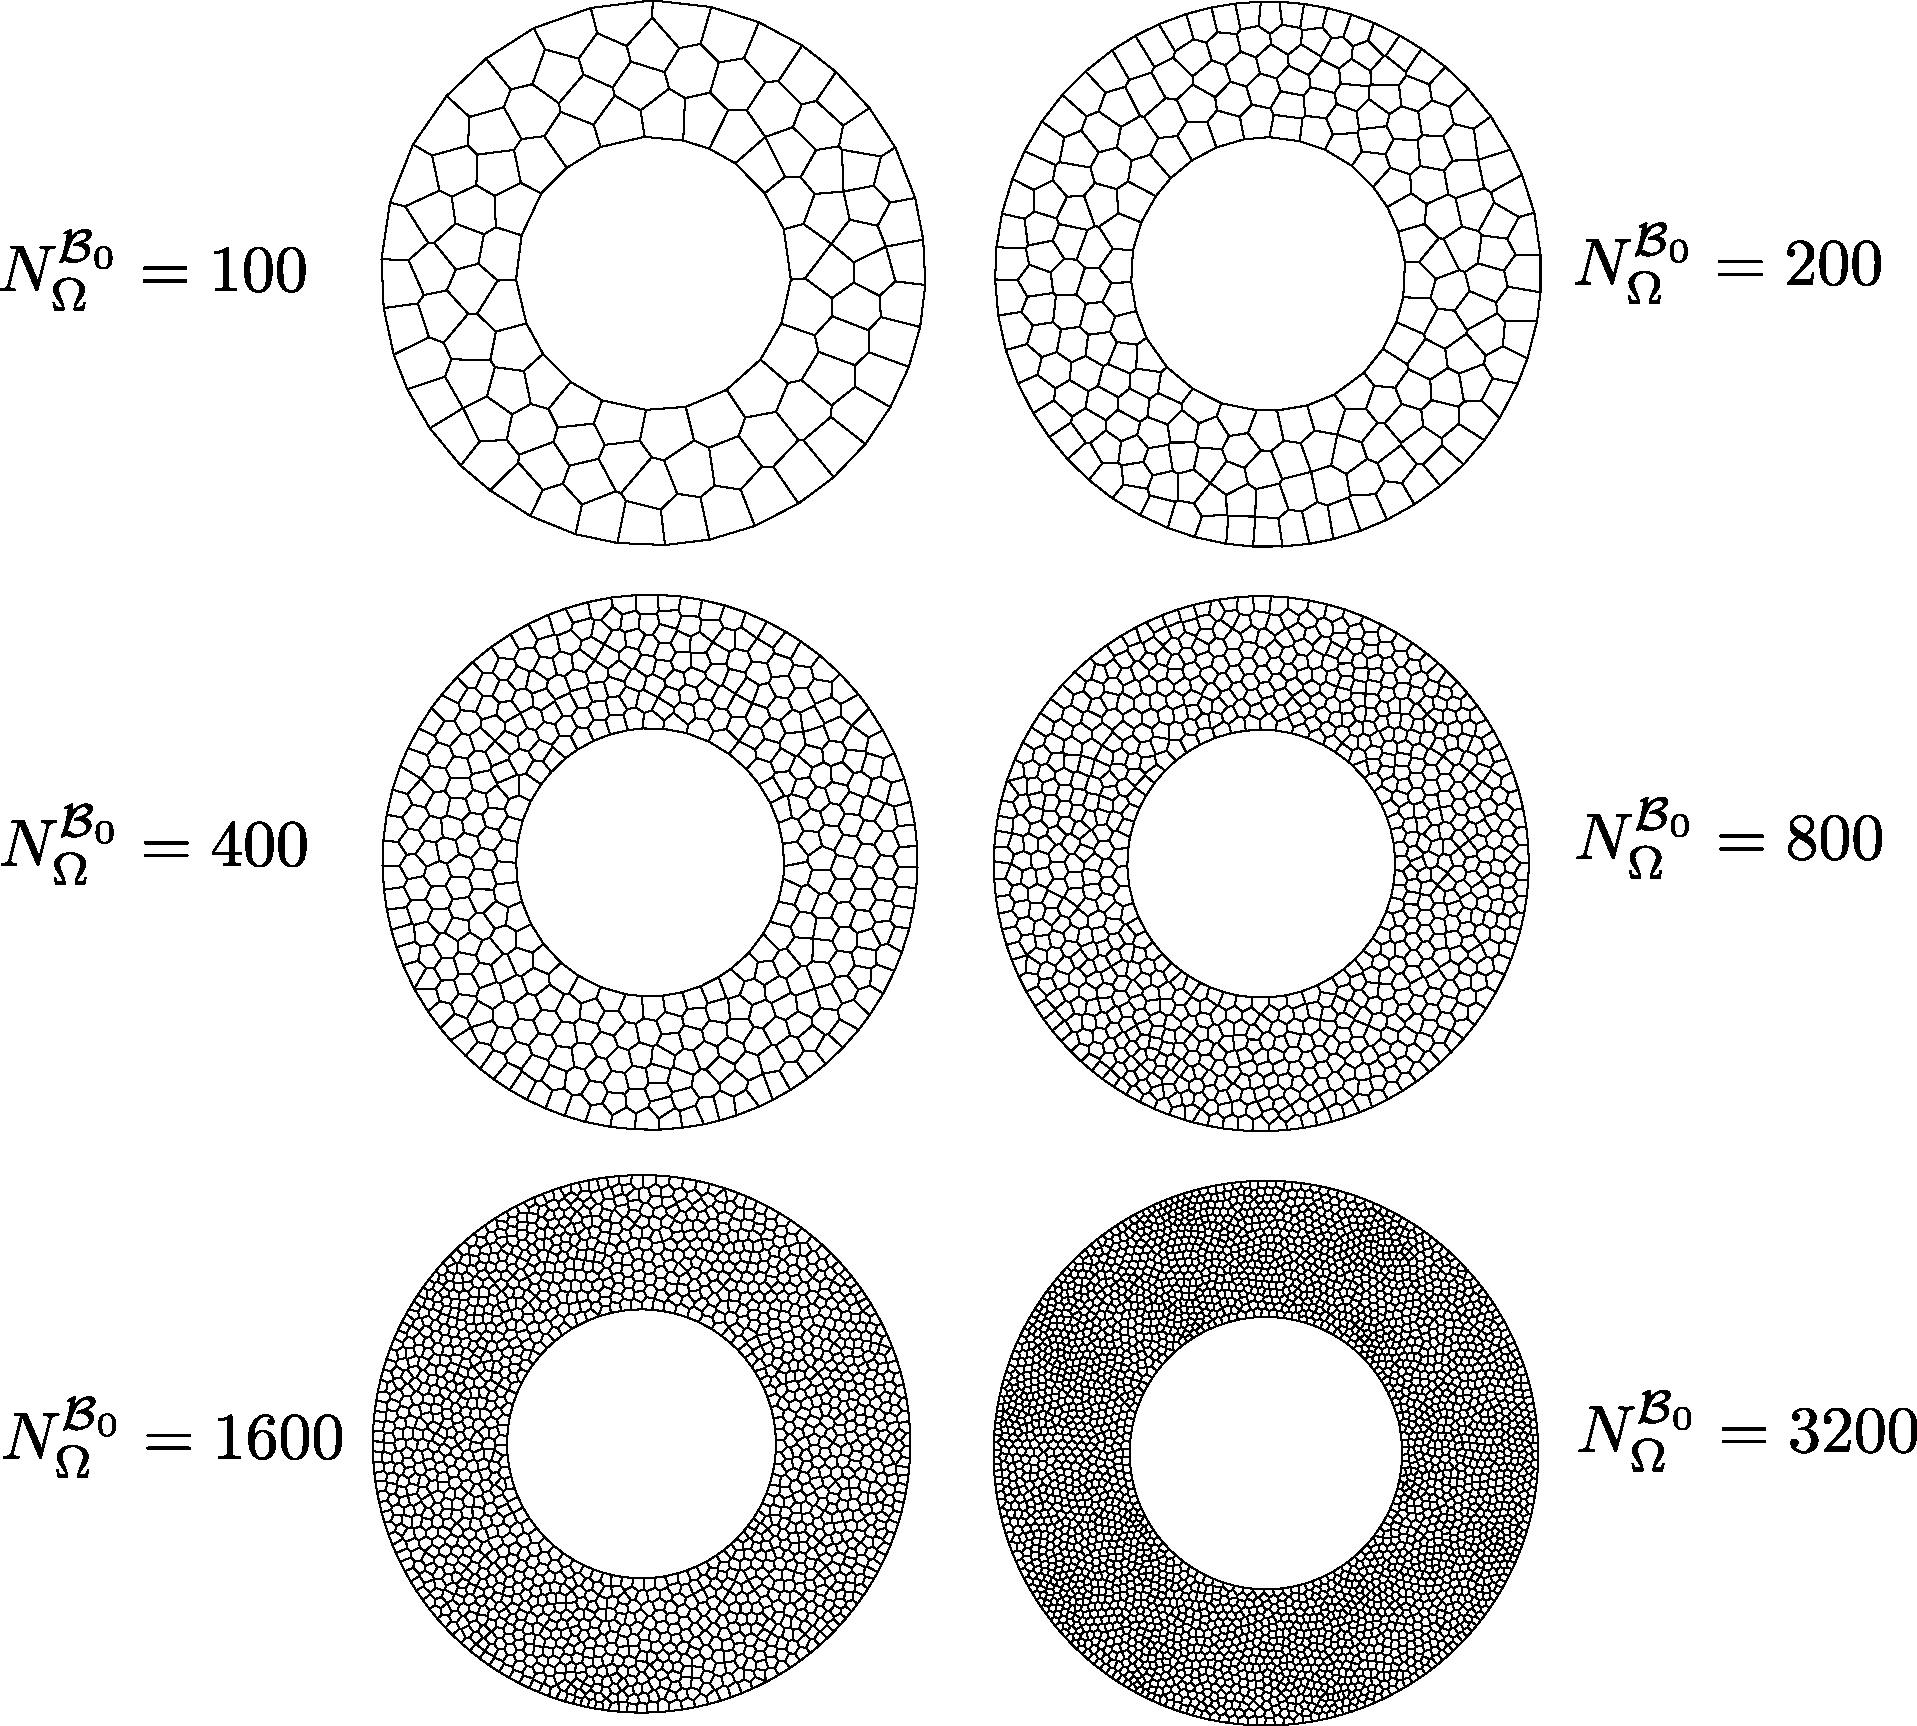
\includegraphics[width=6.0in]{figures/annulus_meshes.pdf}
  \caption{Polygonal meshes with varying levels of refinement for the twisting annulus problem.}
  \label{fig:annulus_meshes}
\end{figure}

\begin{figure}[!h]
  \centering
  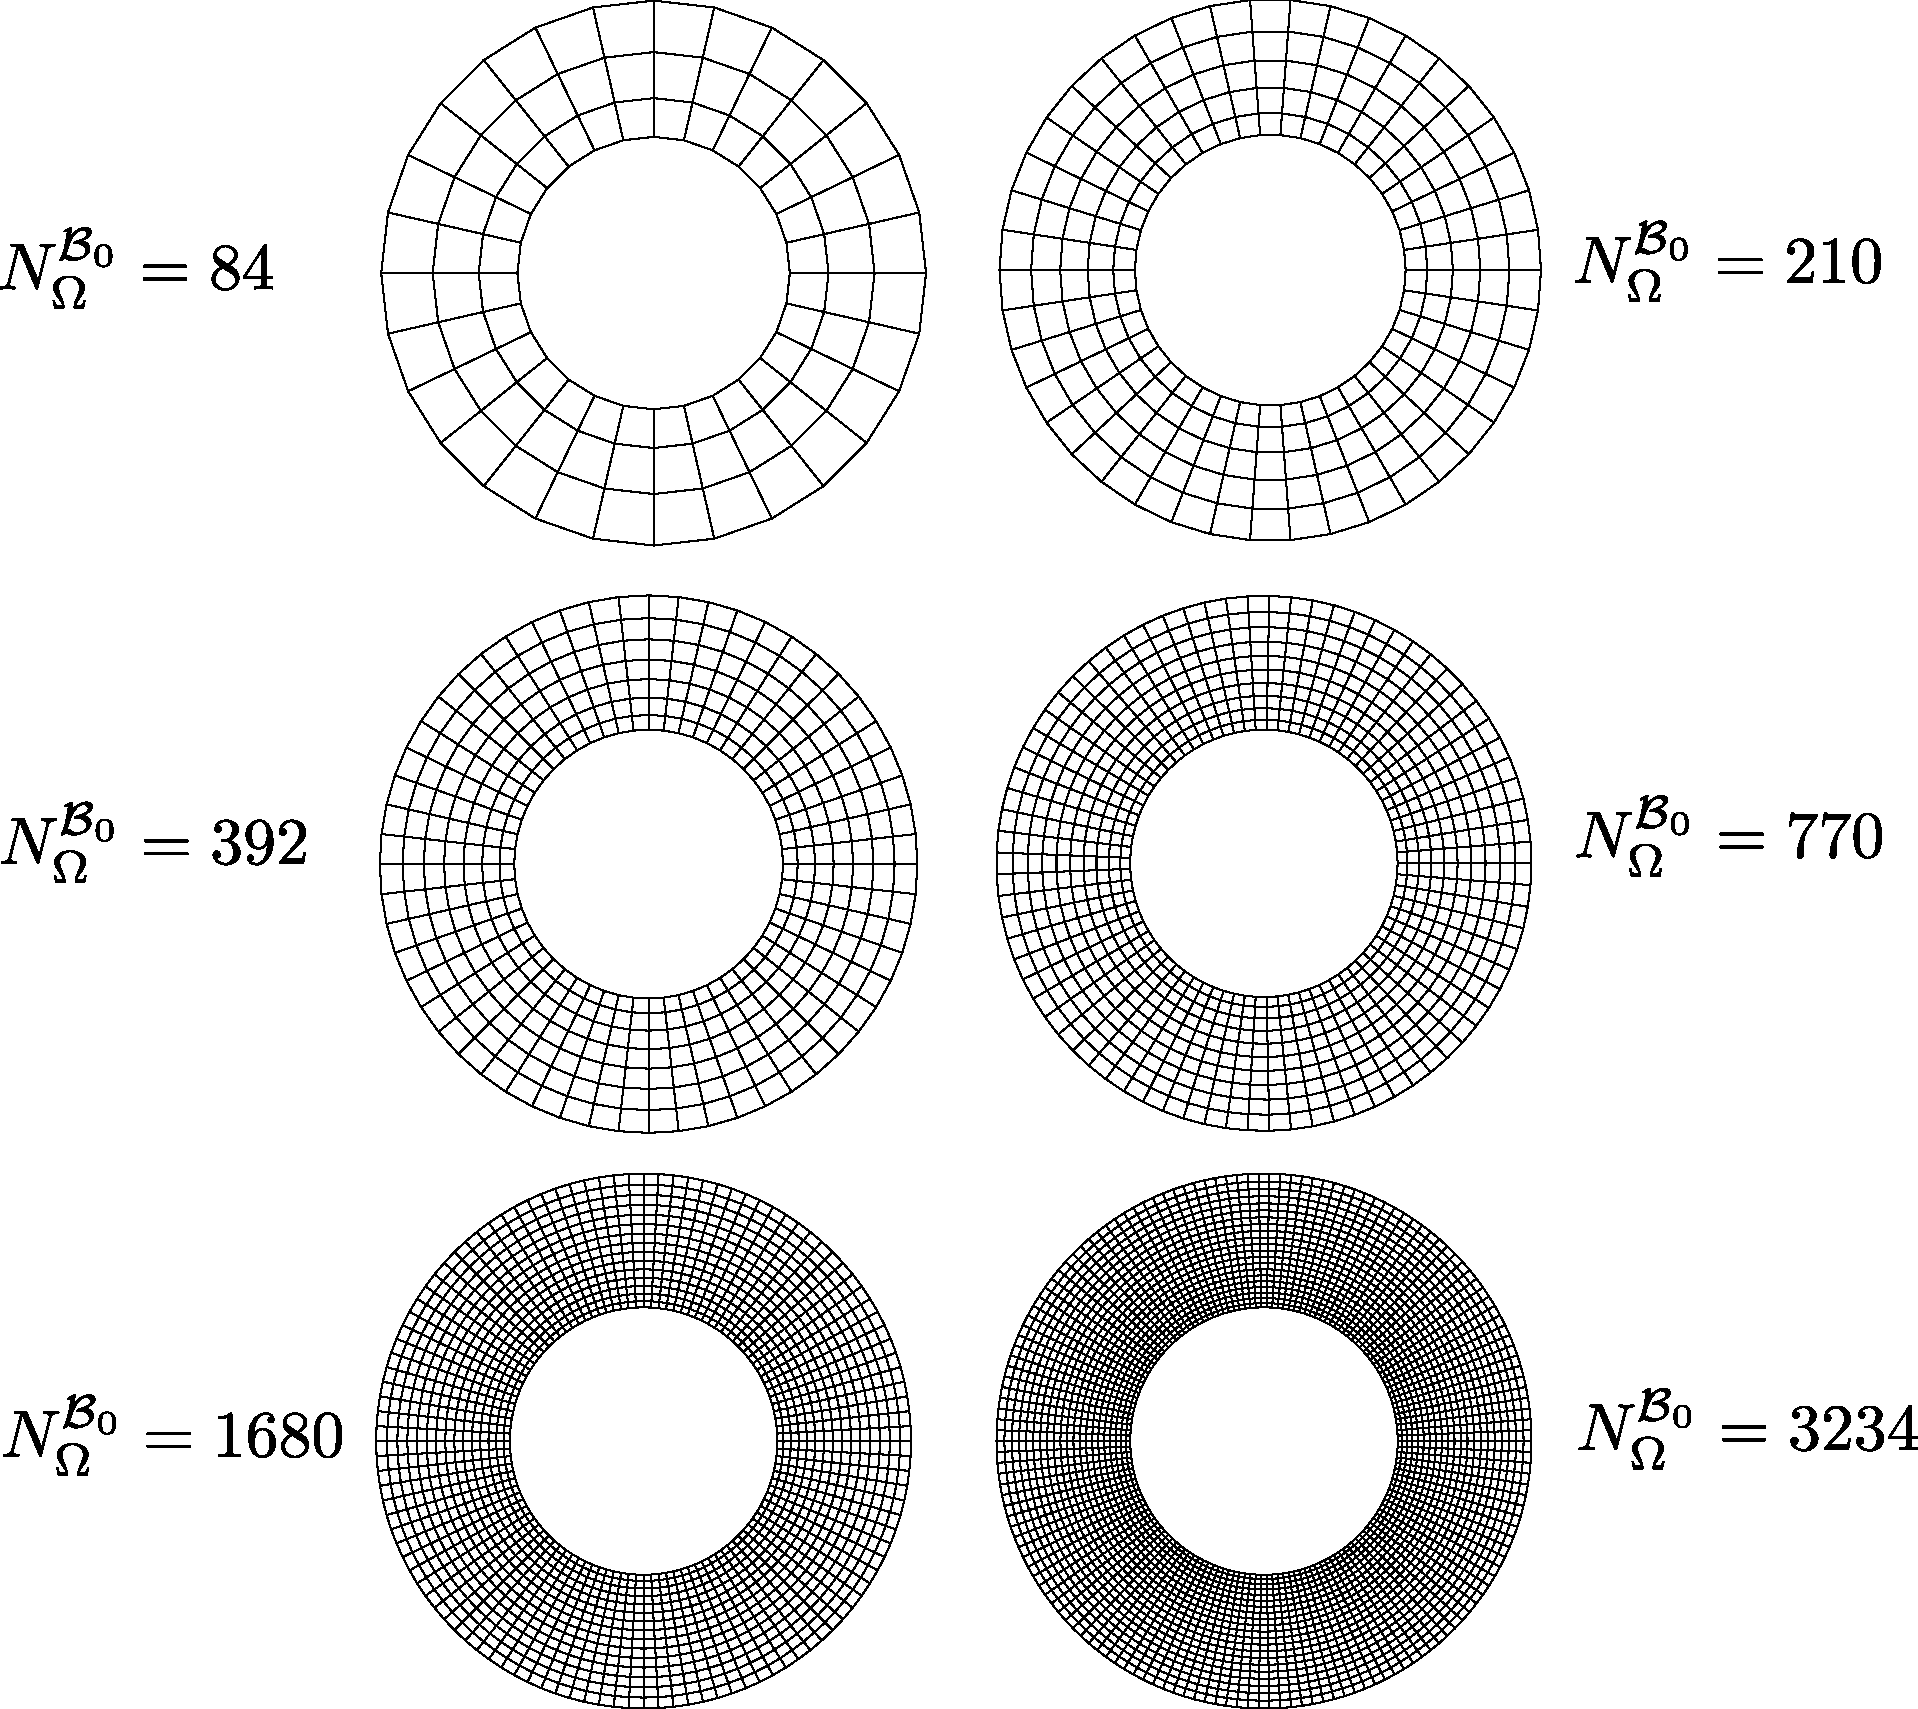
\includegraphics[width=6.0in]{figures/quad_annulus_meshes.pdf}
  \caption{Quadrilateral meshes with varying levels of refinement for the twisting annulus problem.}
  \label{fig:quad_annulus_meshes}
\end{figure}

\begin{figure}[!h]
  \centering
    \begin{subfigure}[b]{0.49\linewidth}
            \centering
            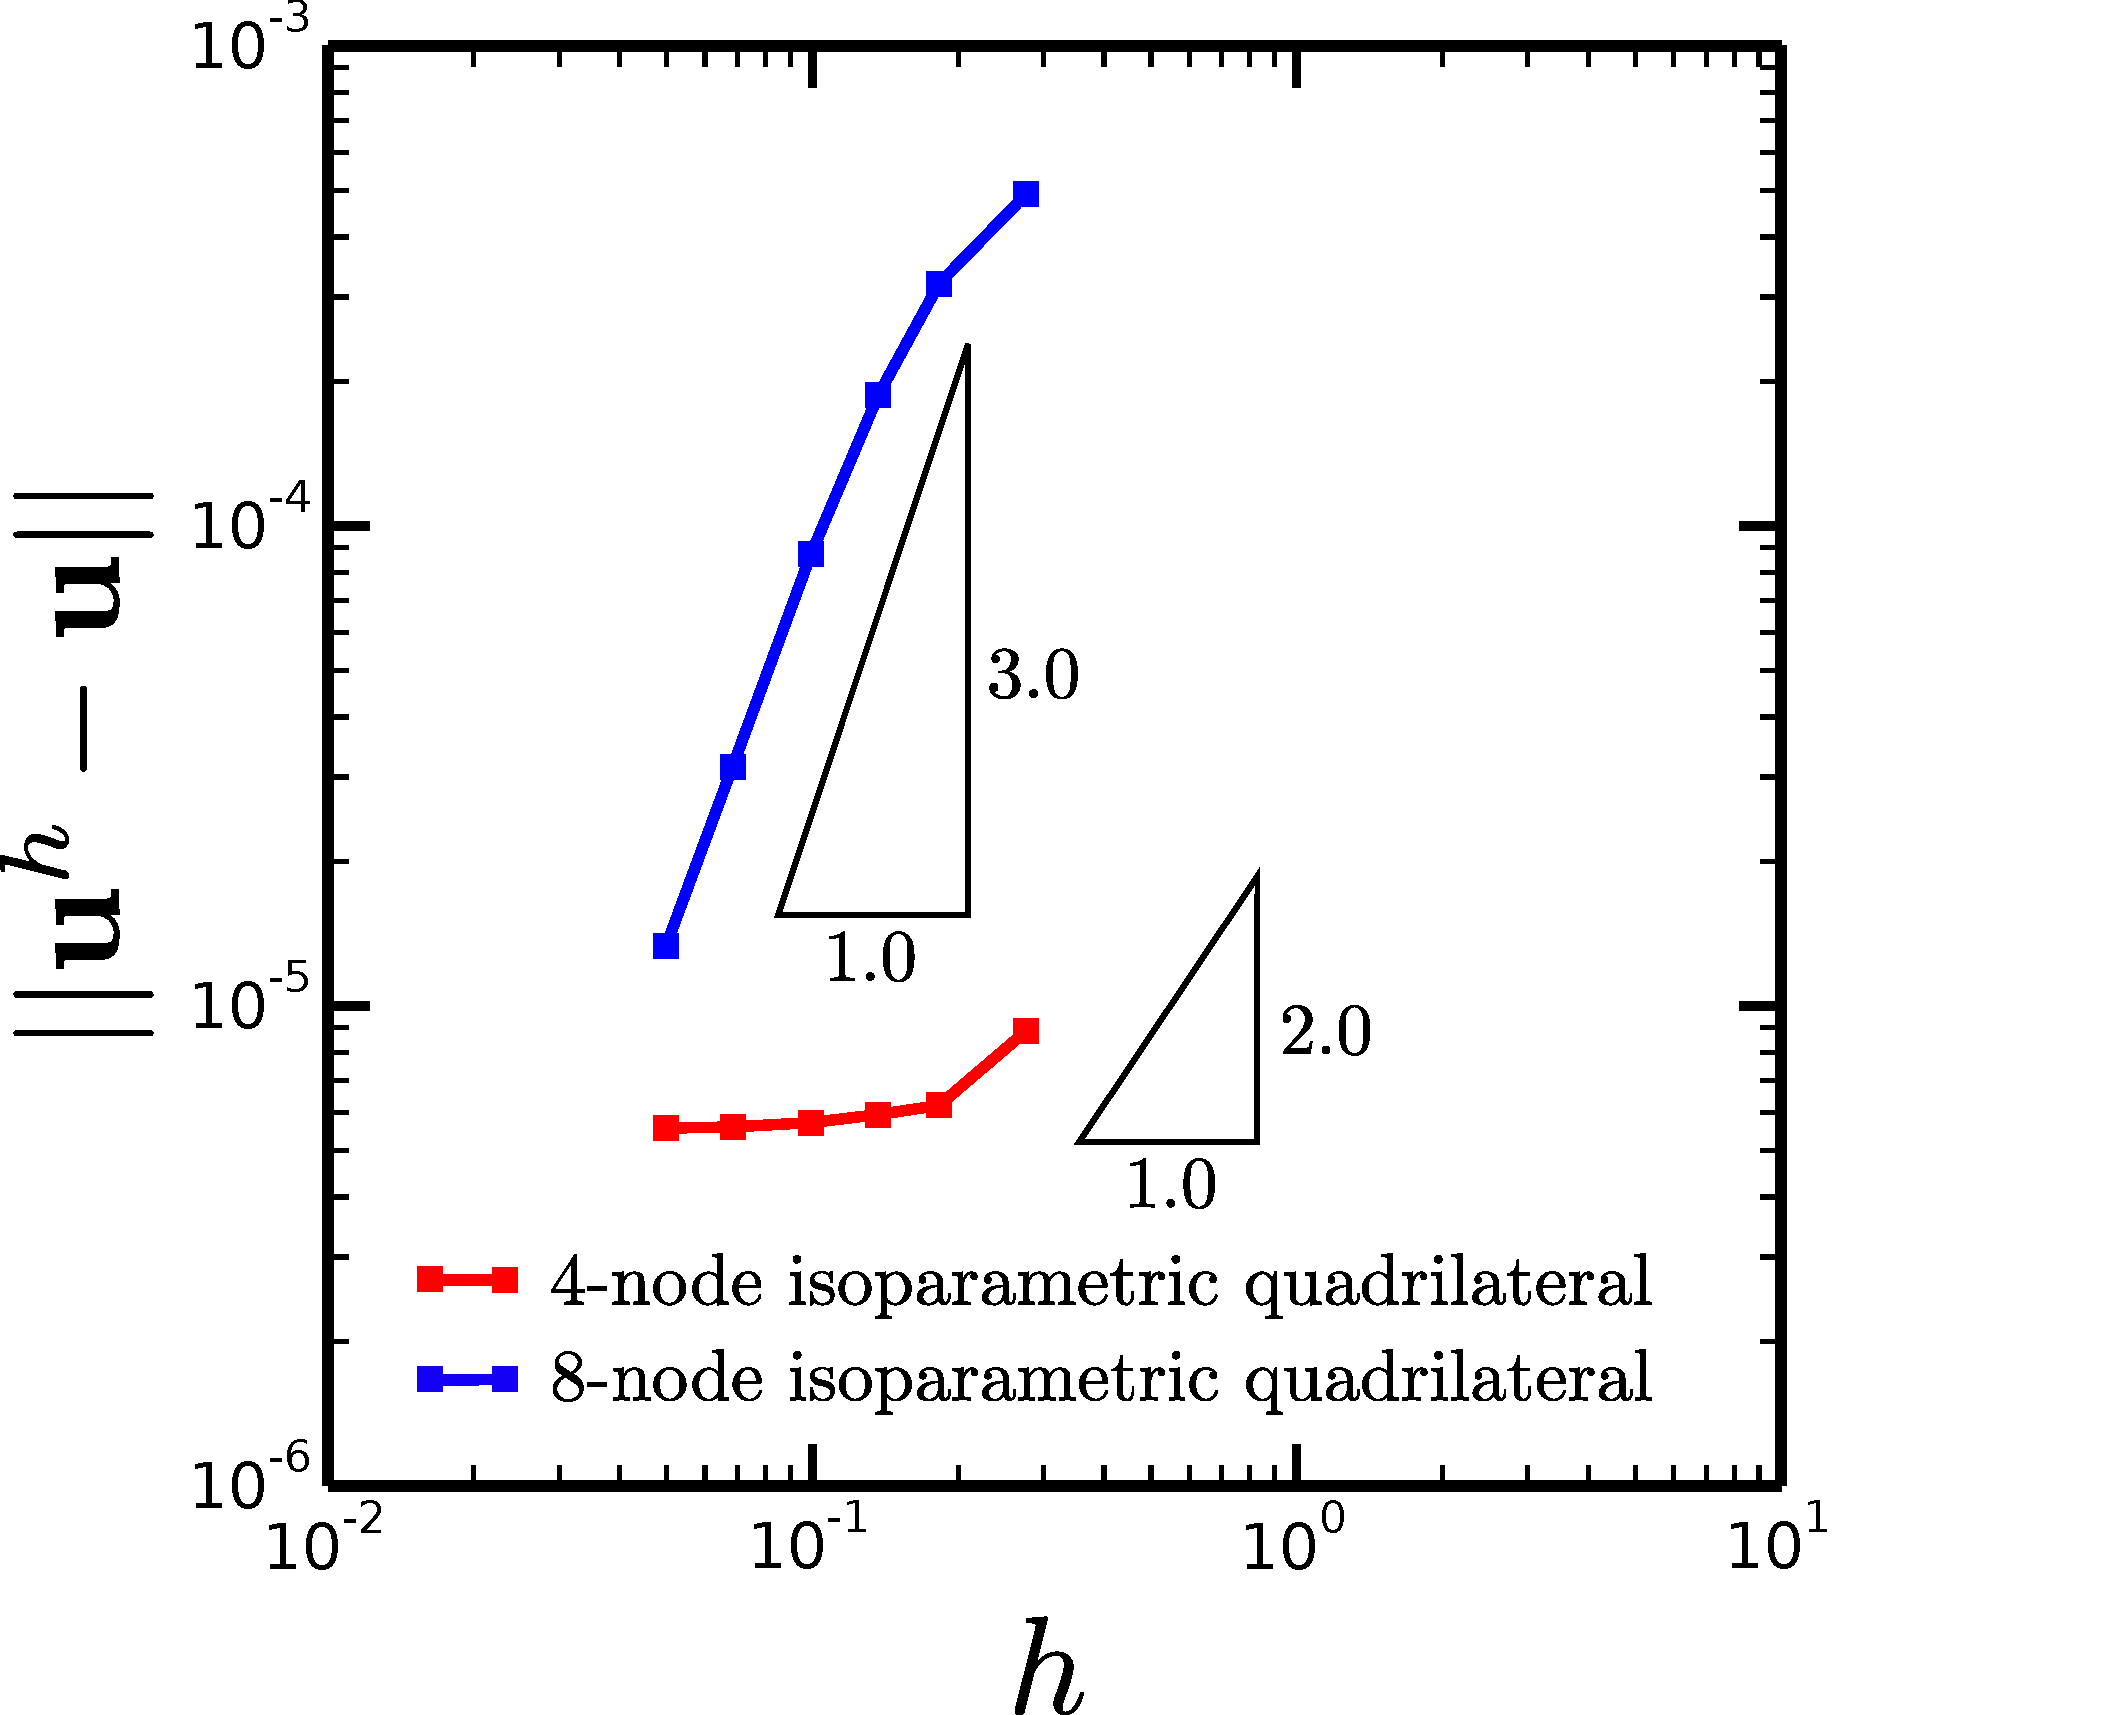
\includegraphics[width=3.3in]{figures/quad_l2_error.pdf}
    			\caption{displacement error \label{fig:quad_l2_error}}
    \end{subfigure}
	\begin{subfigure}[b]{0.49\linewidth}
            \centering
            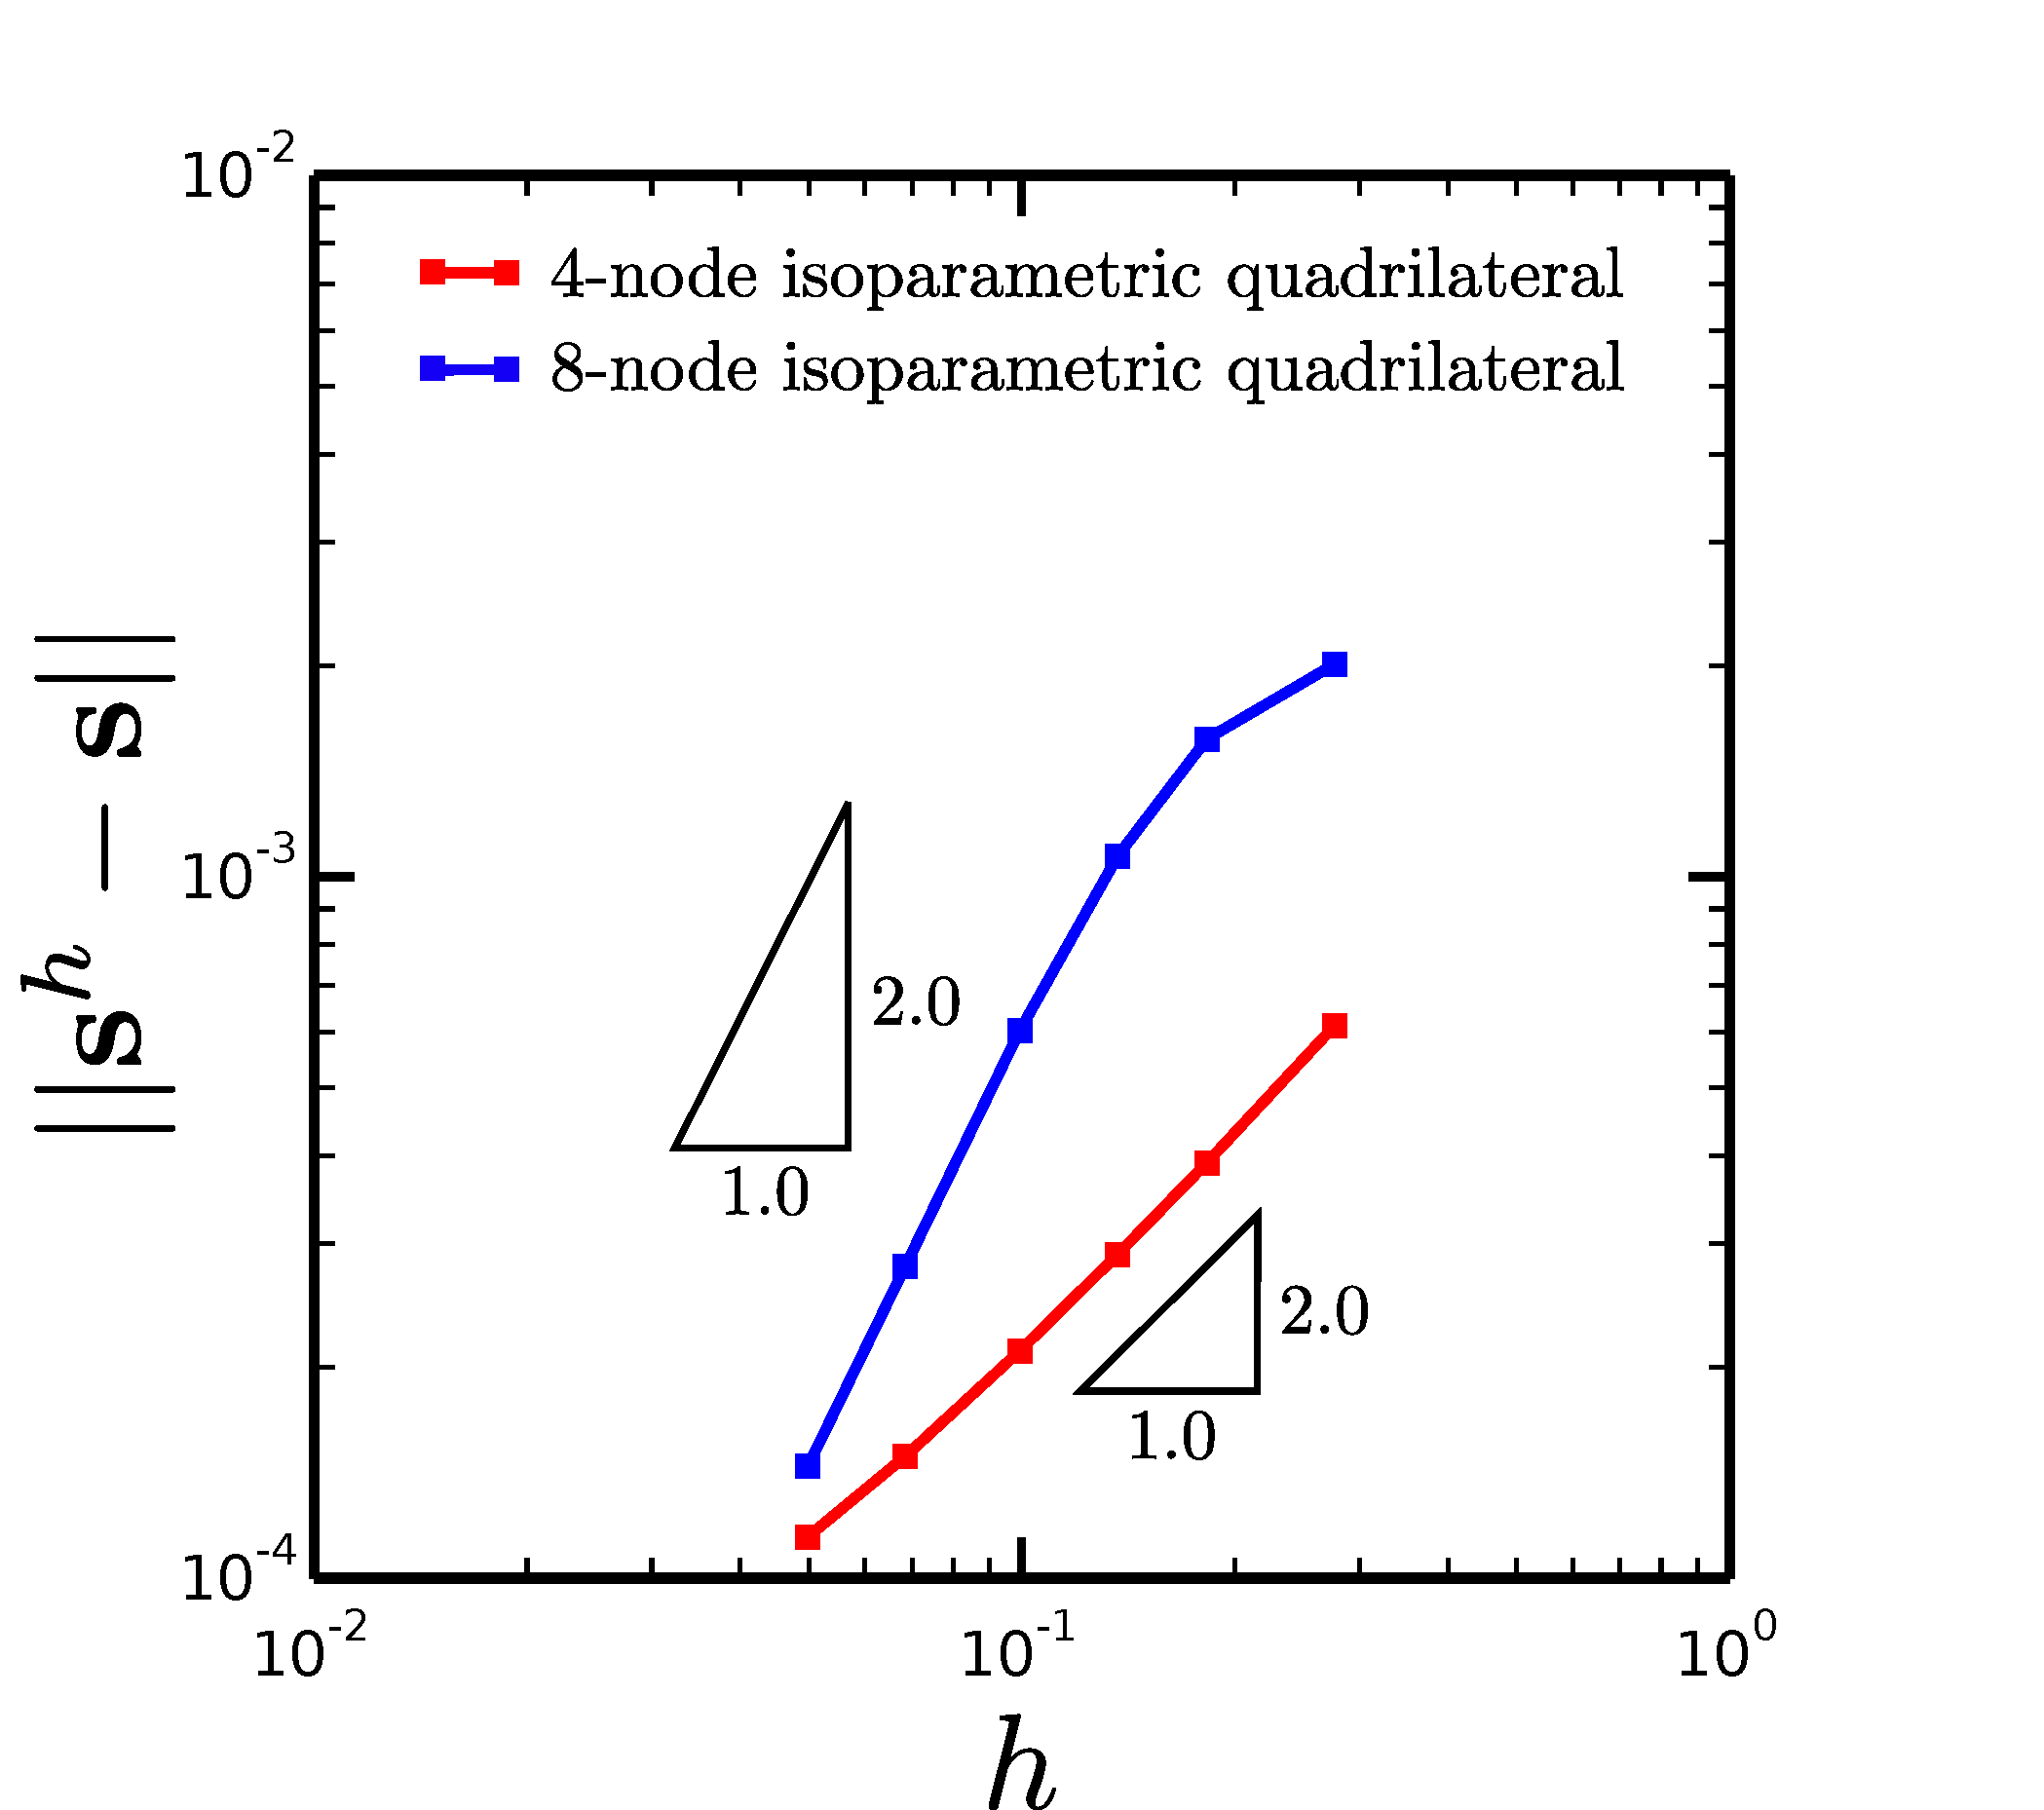
\includegraphics[width=3.3in]{figures/quad_h1_error.pdf}
    			\caption{stress deviator error \label{fig:quad_h1_error}}
    \end{subfigure} \caption{Convergence plots for the twisting annulus problem using standard isoparametric elements.}
  \label{fig:quad_error}
\end{figure}

\begin{figure}[!h]
  \centering
    \begin{subfigure}[b]{0.49\linewidth}
            \centering
            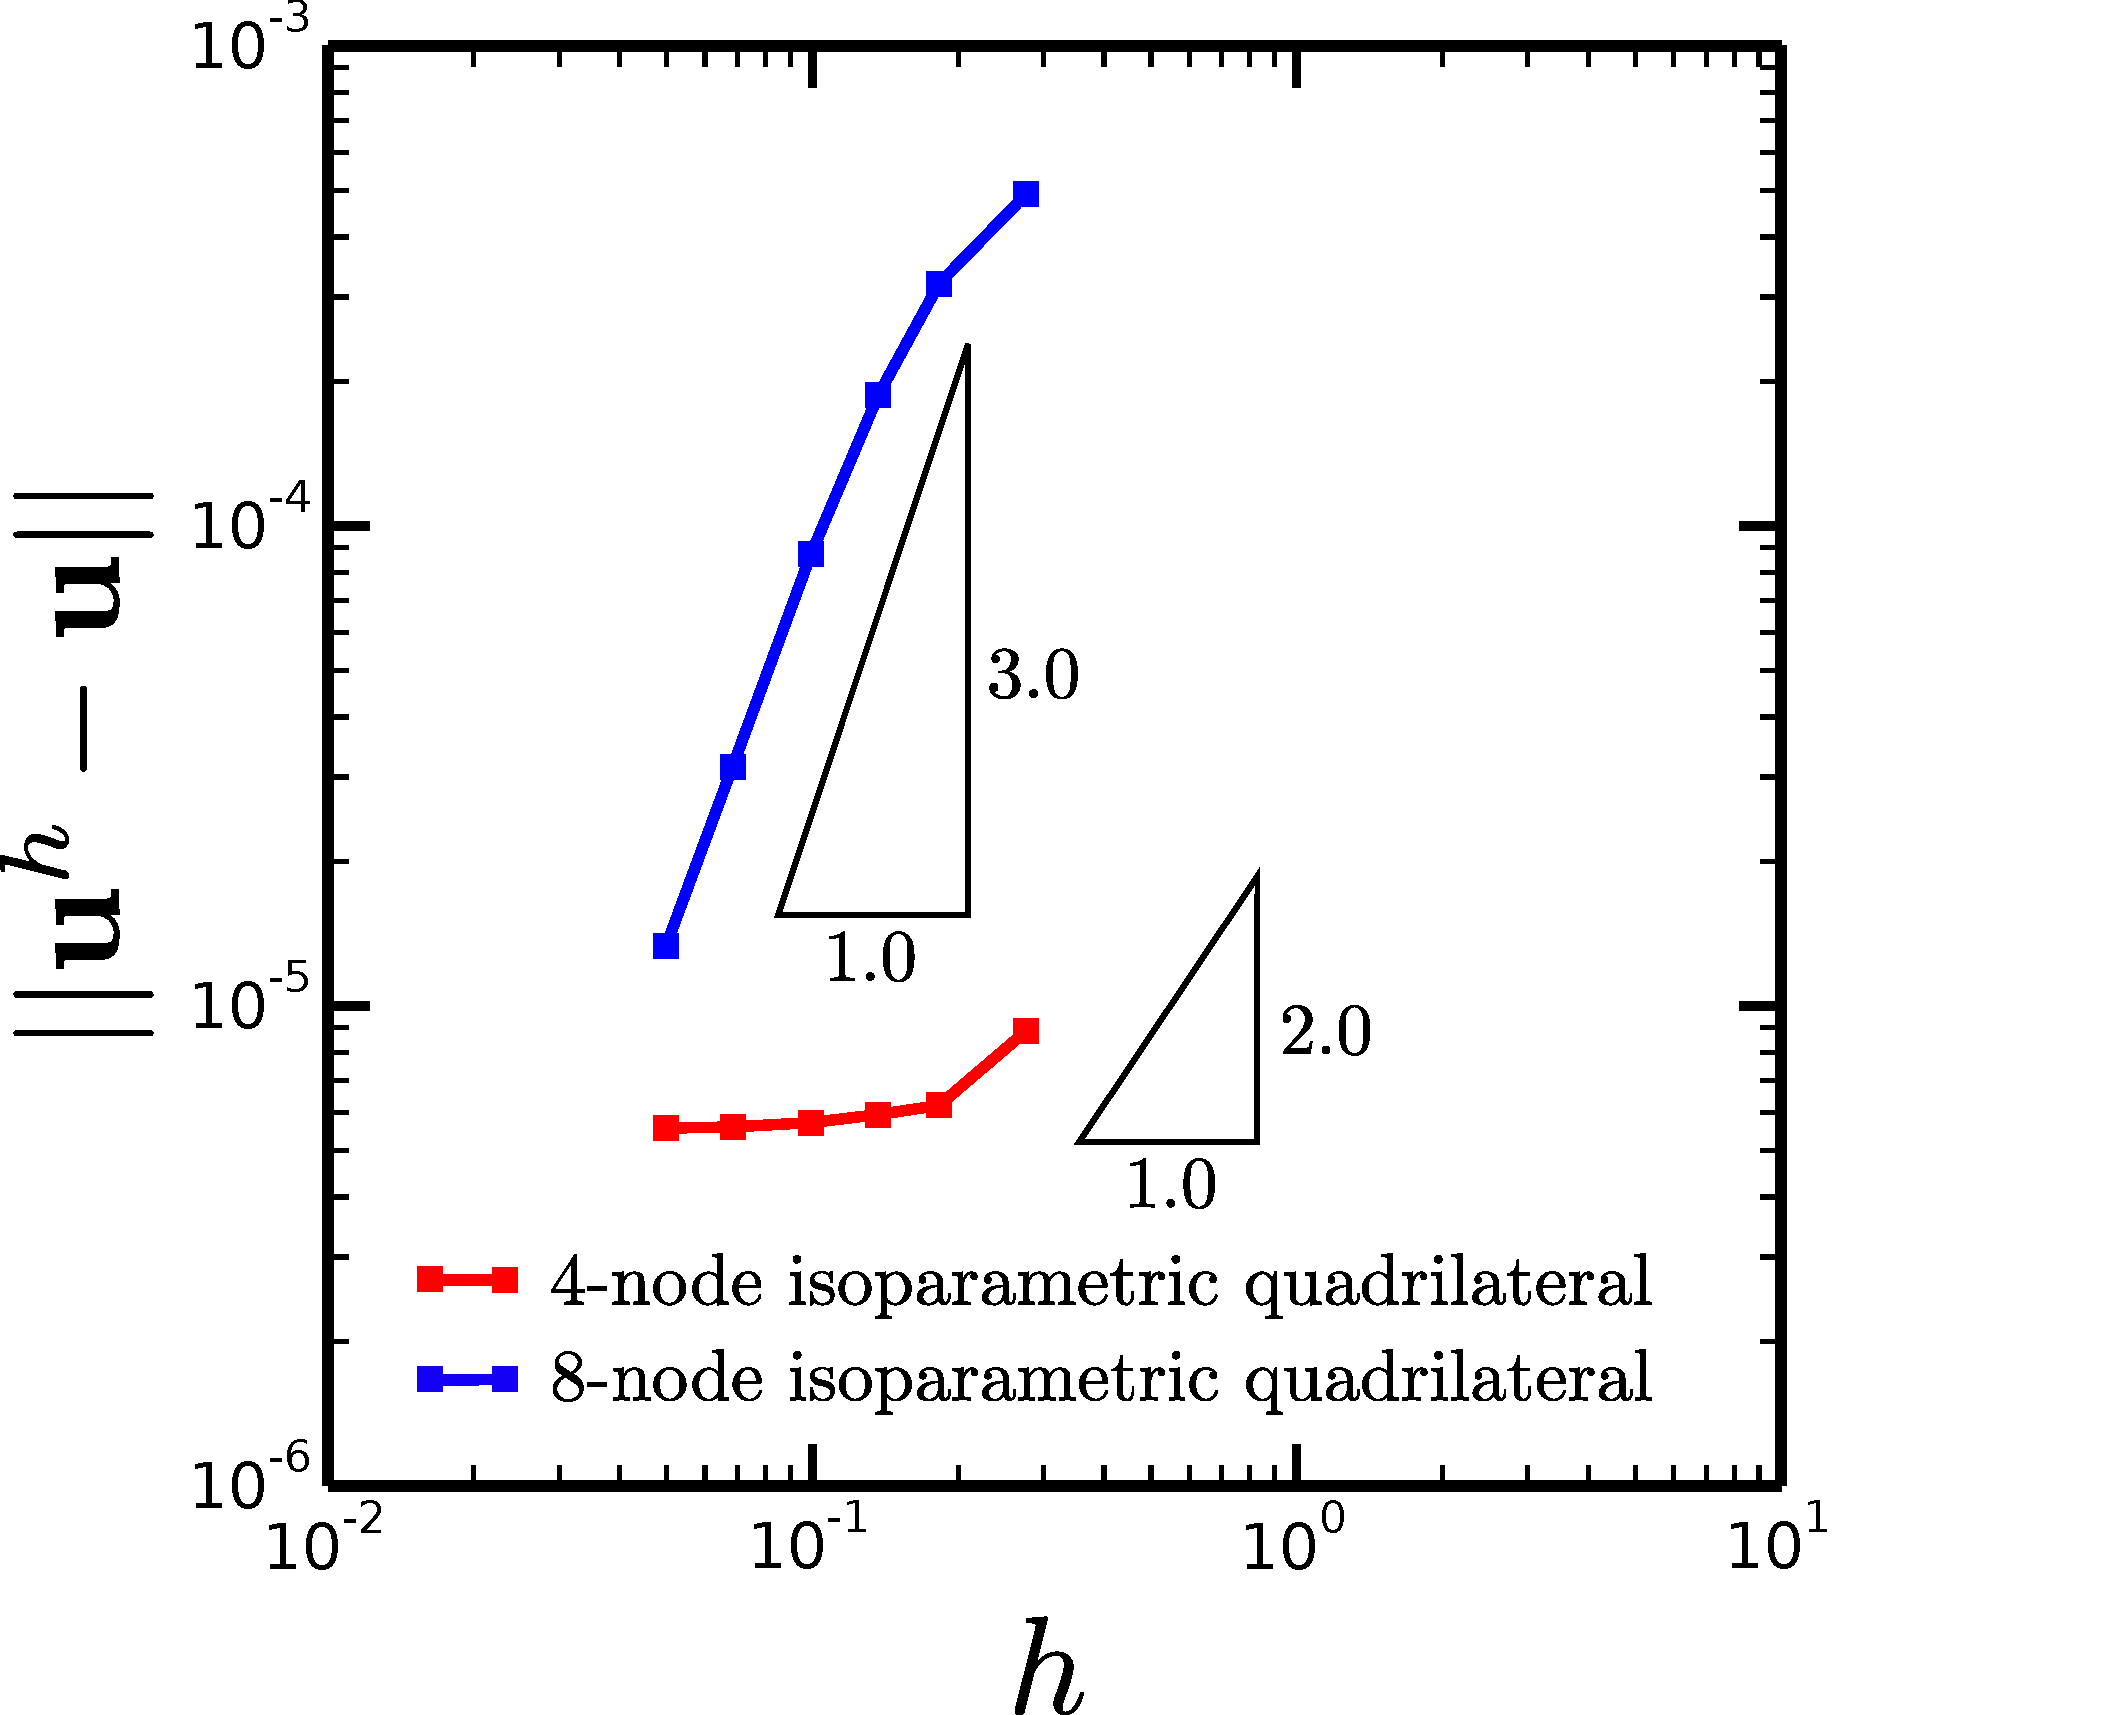
\includegraphics[width=3.3in]{figures/quad_l2_error.pdf}
    			\caption{displacement error \label{fig:quad_l2_error}}
    \end{subfigure}
	\begin{subfigure}[b]{0.49\linewidth}
            \centering
            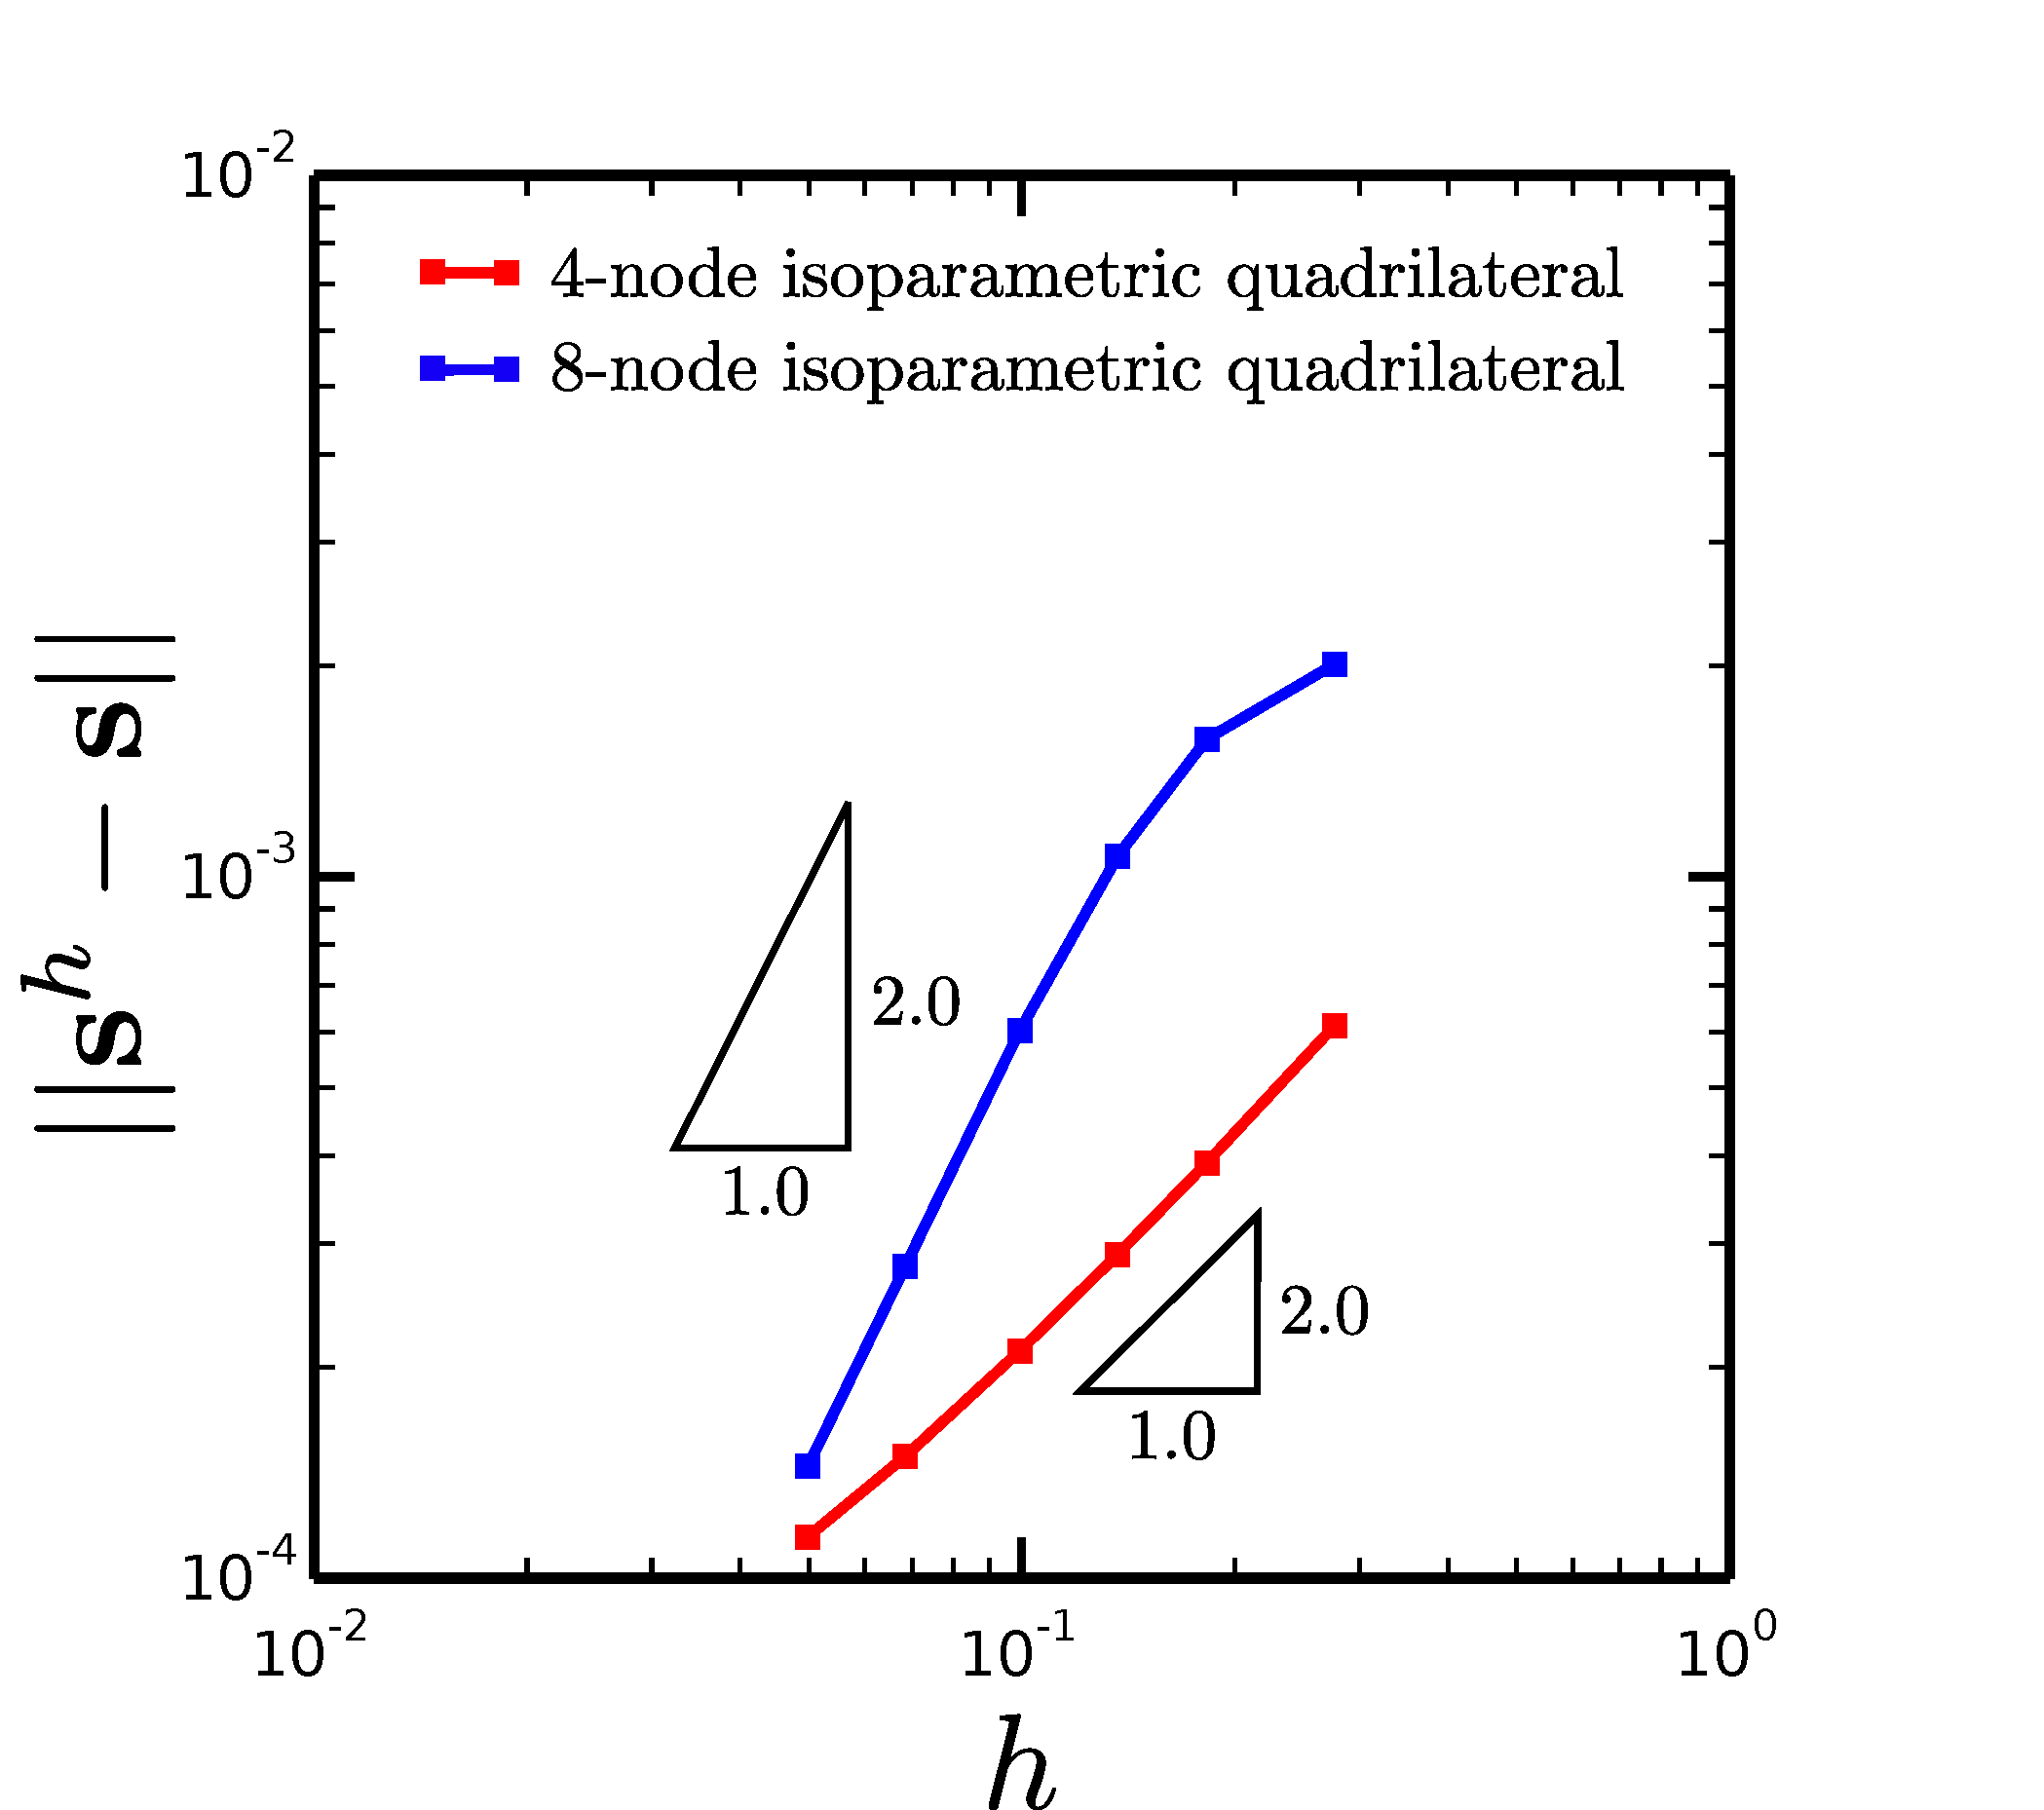
\includegraphics[width=3.3in]{figures/quad_h1_error.pdf}
    			\caption{stress deviator error \label{fig:quad_h1_error}}
    \end{subfigure} \caption{Convergence plots for the twisting annulus problem using standard isoparametric elements.}
  \label{fig:quad_error}
\end{figure}

\subsection*{Thin Corner-Supported Plate}

Consider a thin plate 
(Description of the corner-supported plate problem).

\begin{figure}[!h]
  \centering
  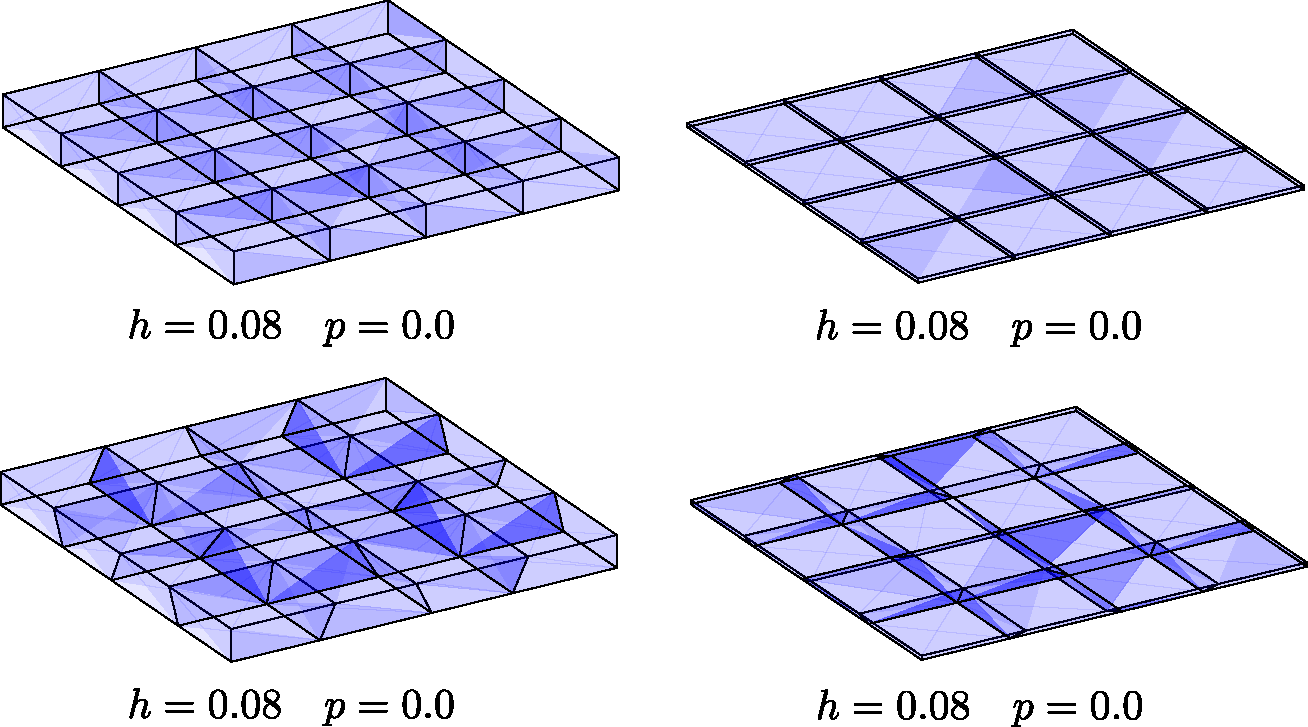
\includegraphics[width=6.0in]{figures/plate_meshes.pdf}
  \caption{Hexahedral meshes with variable plate thickness $h$ and mesh perturbations $p$ for the corner-supported plate problem.}
  \label{fig:plate_meshes}
\end{figure}

\subsubsection{Exact Solution}

An exact solution for the vertical displacement field of the plate prob

\section{Comparison with Isoparametric Finite Elements}

\subsection*{Ductile Necking}

\begin{figure}[!h]
    \centering
    \begin{subfigure}[b]{0.49\linewidth}
            \centering
            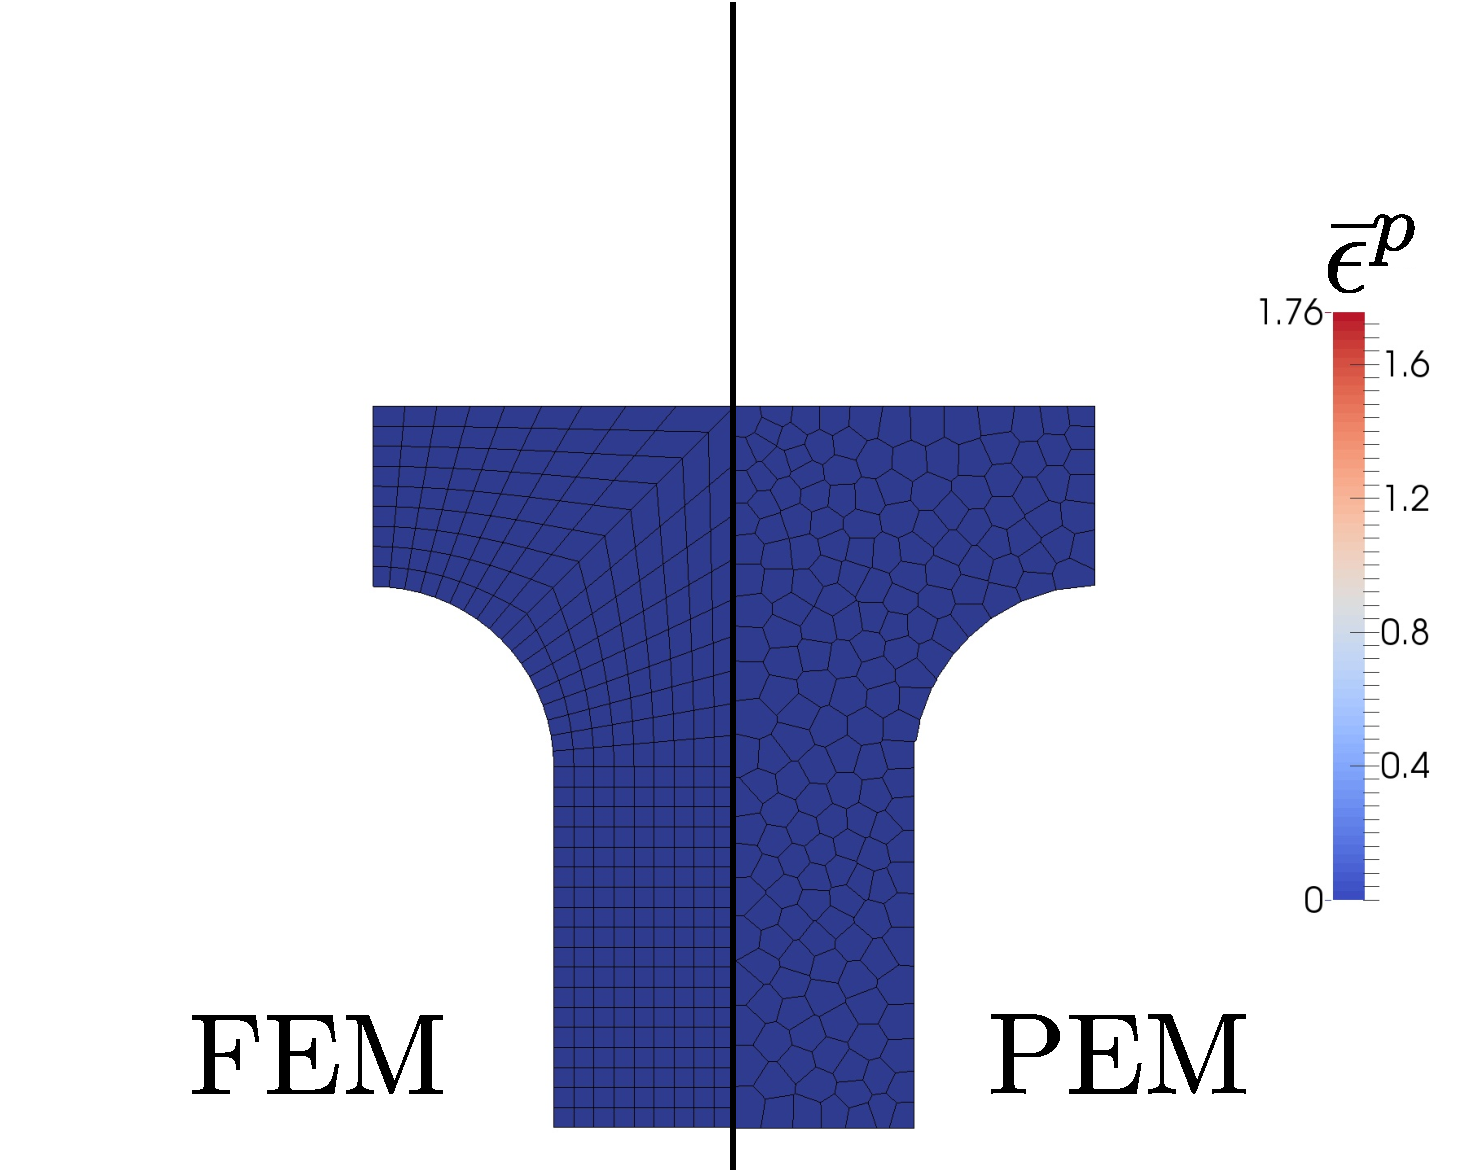
\includegraphics[width=3.0in]{figures/necking_eqps_0.pdf}
    			\caption{$t=0.0$ \label{fig:necking_eqps_0}}
    \end{subfigure}
	\begin{subfigure}[b]{0.49\linewidth}
            \centering
            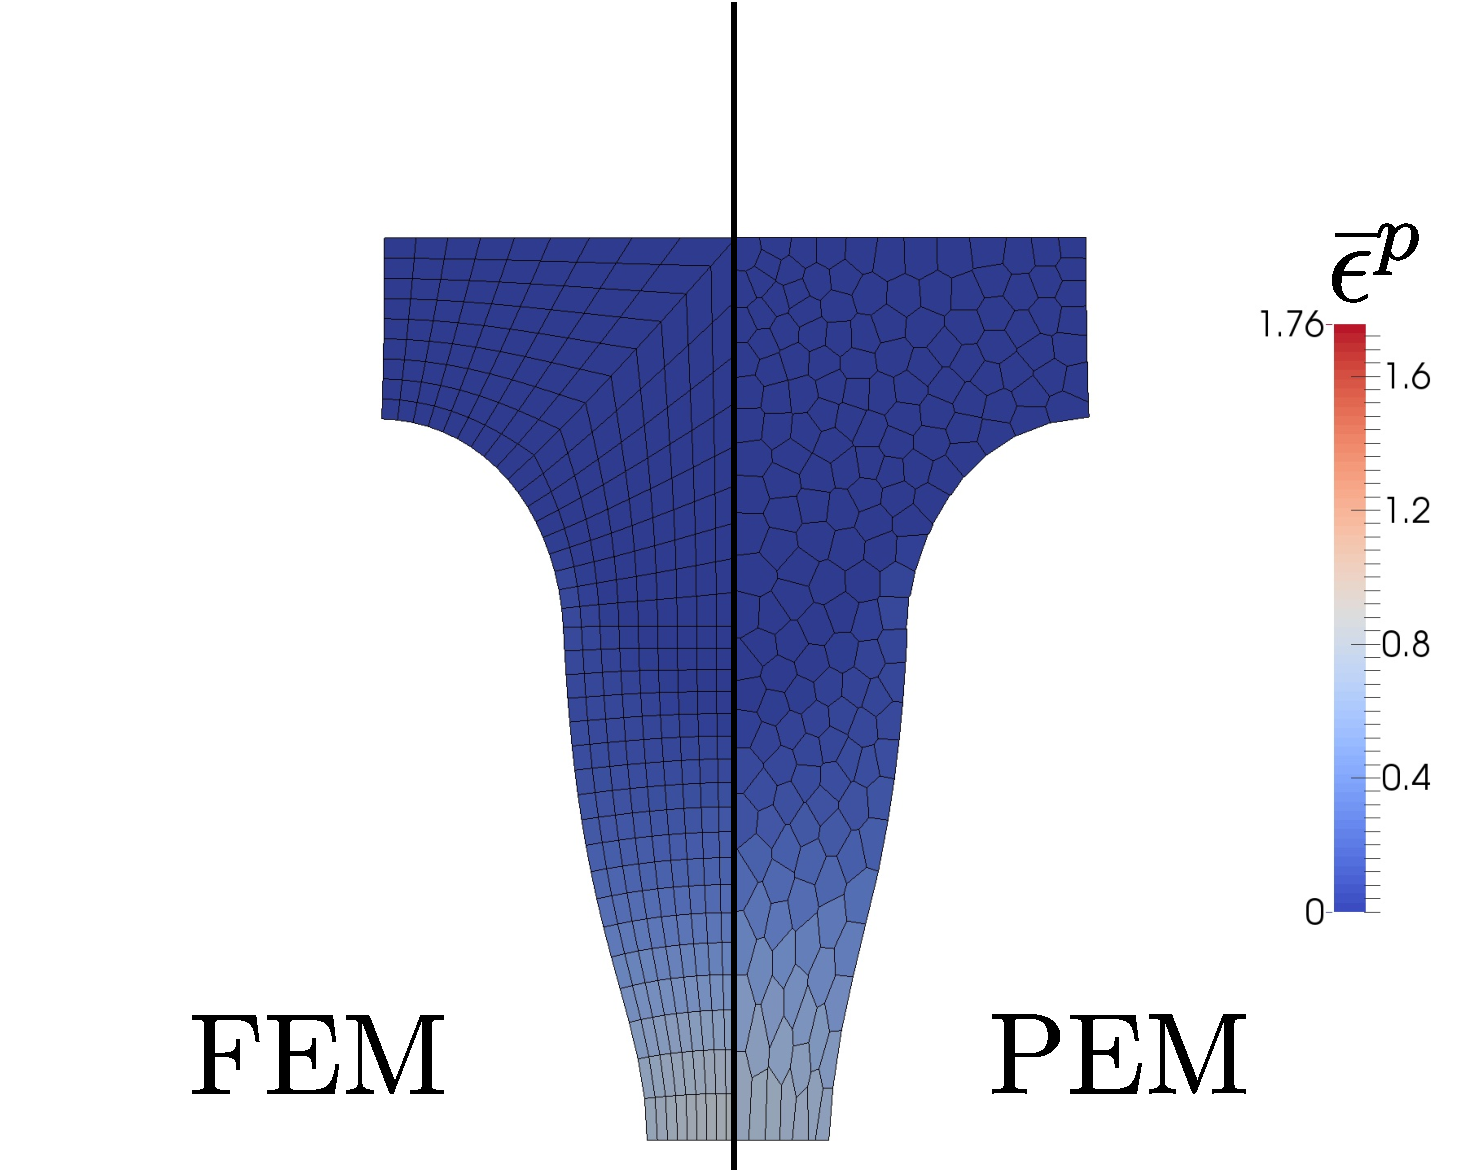
\includegraphics[width=3.0in]{figures/necking_eqps_1.pdf}
    			\caption{$t=0.5$ \label{fig:necking_eqps_1}}
    \end{subfigure}
    \begin{subfigure}[b]{0.49\linewidth}
            \centering
            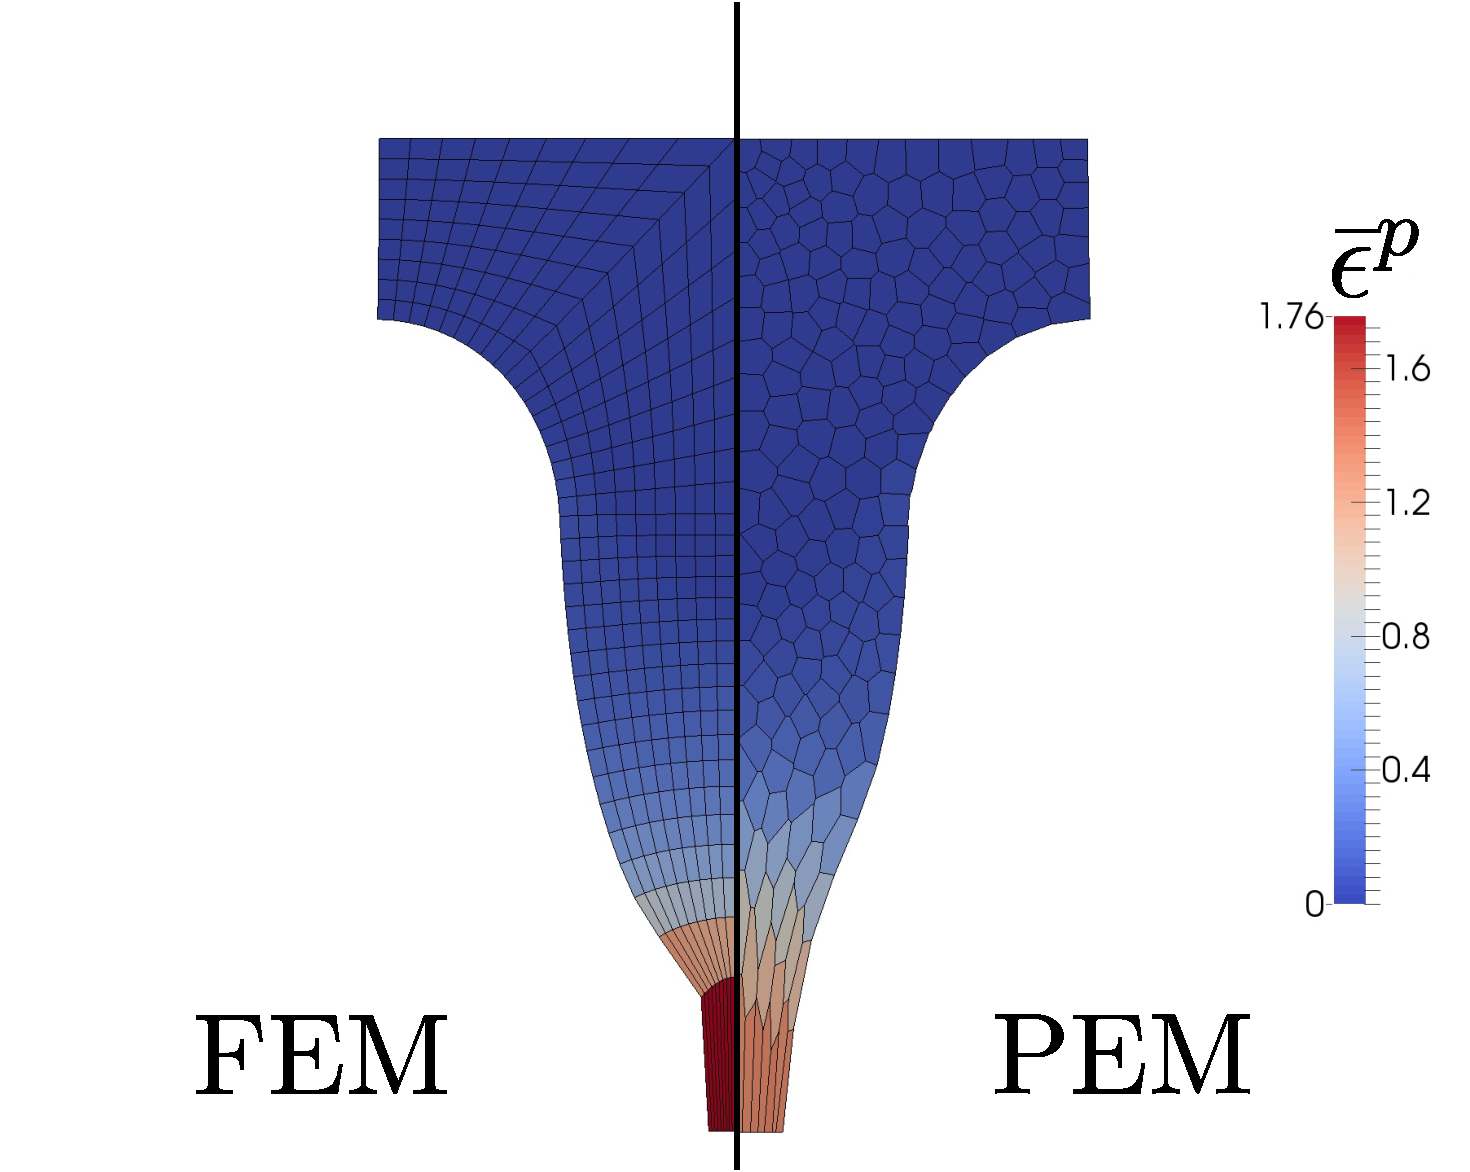
\includegraphics[width=3.0in]{figures/necking_eqps_2.pdf}
    			\caption{$t=0.75$ \label{fig:necking_eqps_2}}
    \end{subfigure}
	\begin{subfigure}[b]{0.49\linewidth}
            \centering
            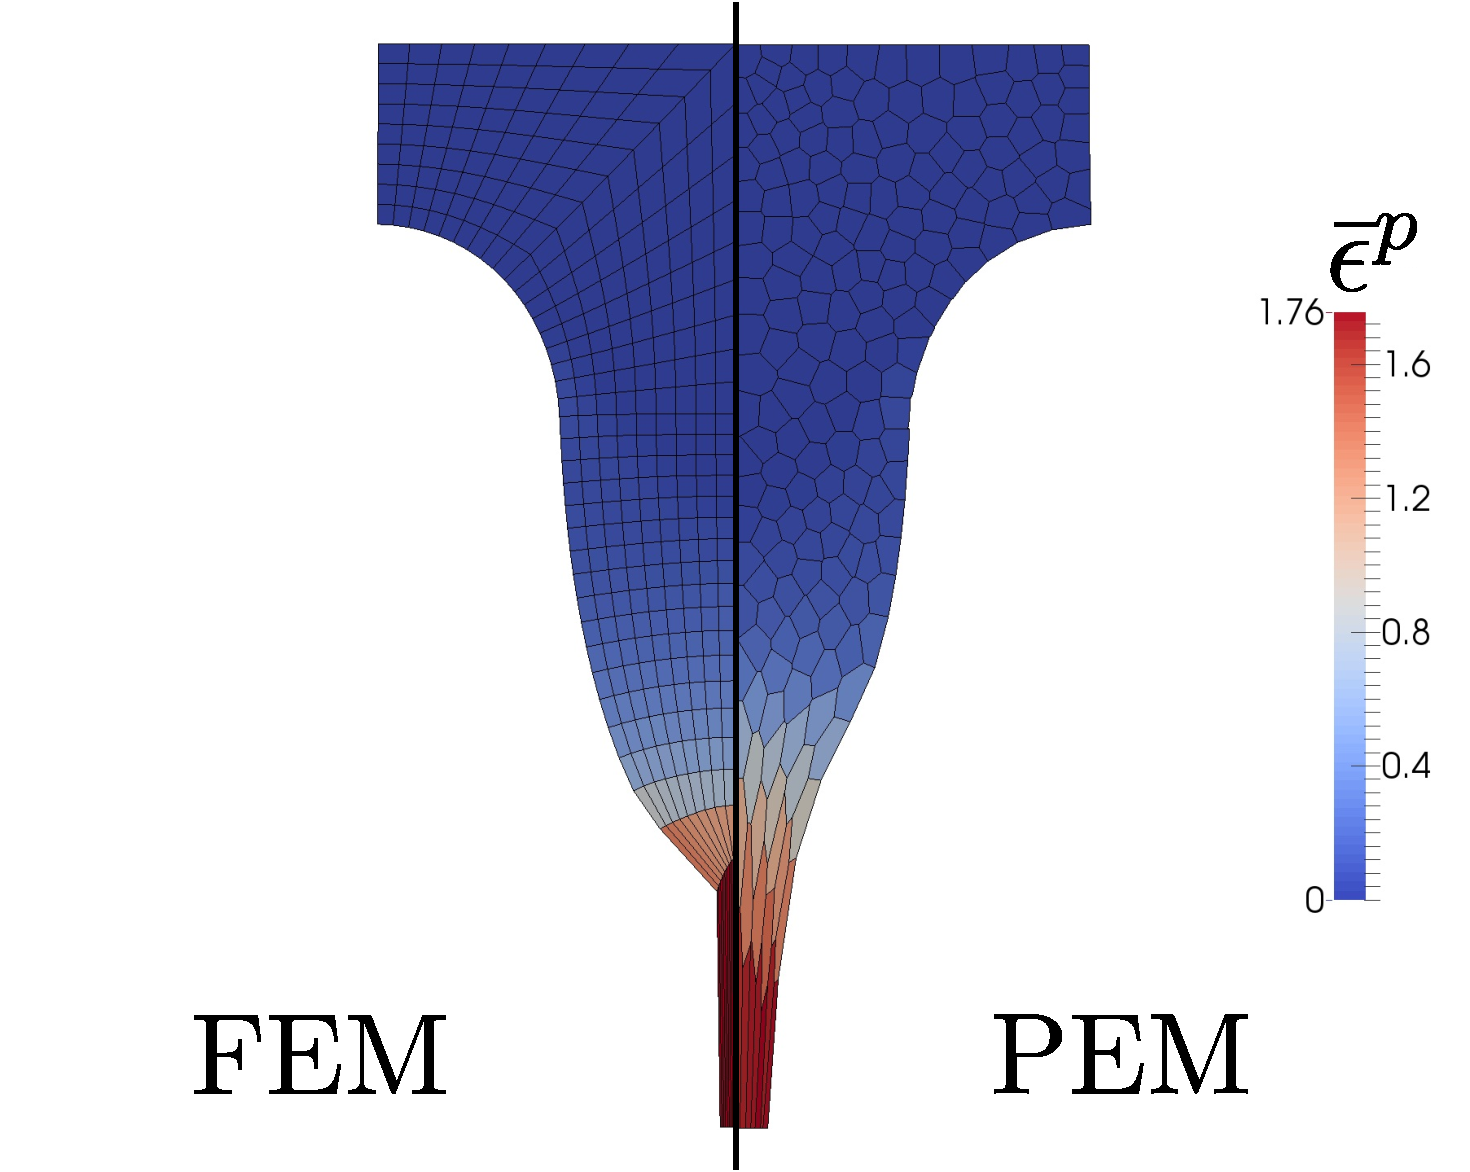
\includegraphics[width=3.0in]{figures/necking_eqps_3.pdf}
    			\caption{$t=1$ \label{fig:necking_eqps_3}}
    \end{subfigure}
    \caption{Comparison of necking behavior at various times during the analysis, depicting deformed shape, and values of equivalent plastic strain.}
\end{figure}

\subsection*{Taylor Bar Dynamic Impact}

\begin{figure}[!h]
  \centering
    \begin{subfigure}[b]{0.49\linewidth}
            \centering
            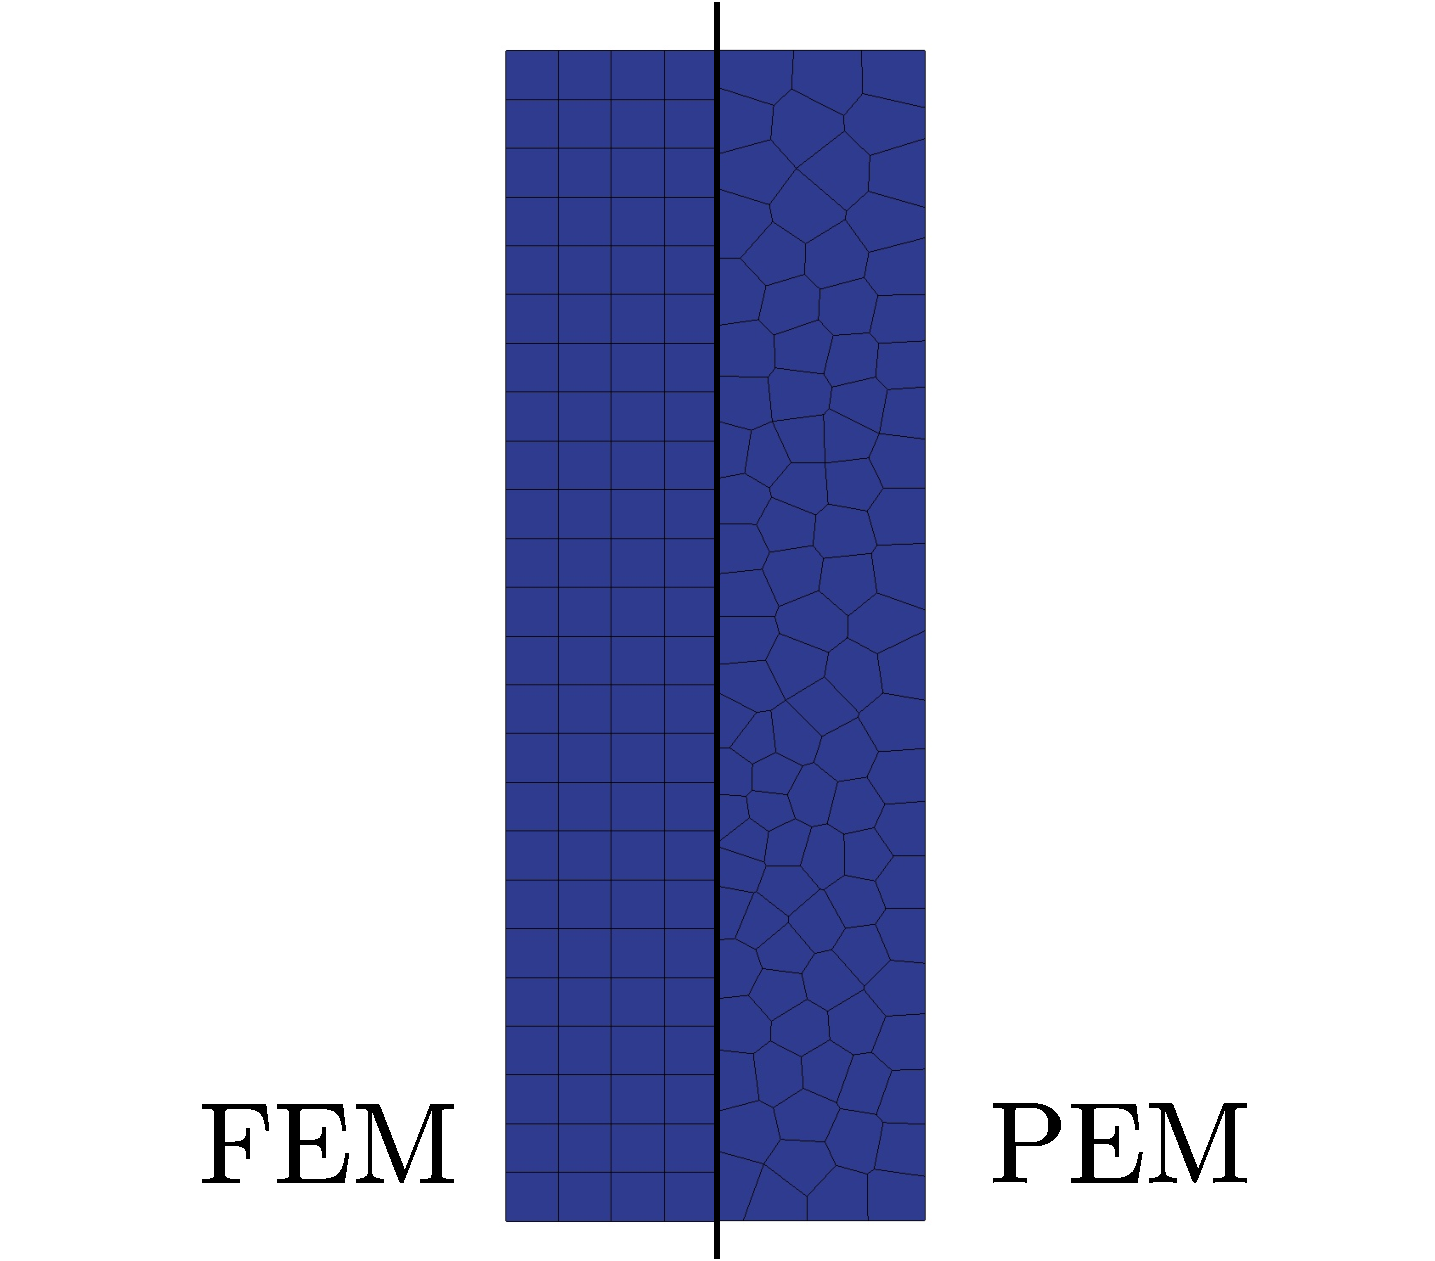
\includegraphics[width=3.0in]{figures/taylor_eqps_0.pdf}
    			\caption{$t=0.0$ \label{fig:taylor_eqps_0}}
    \end{subfigure}
	\begin{subfigure}[b]{0.49\linewidth}
            \centering
            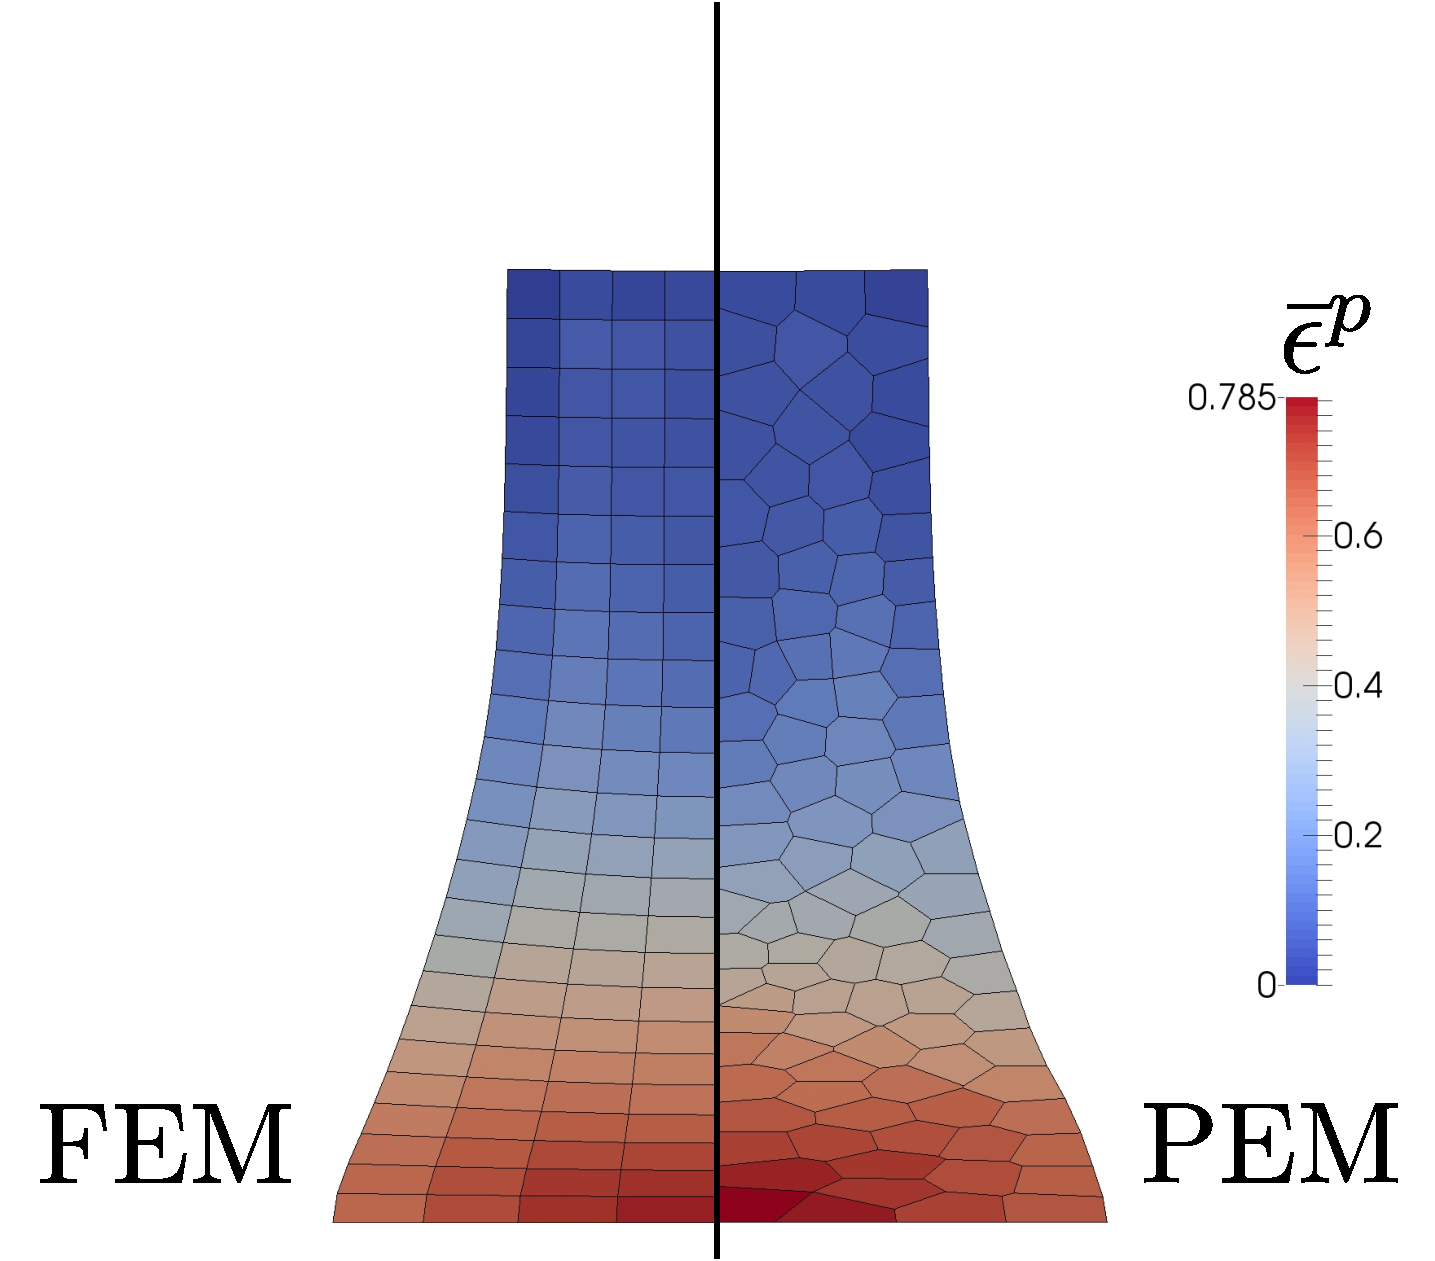
\includegraphics[width=3.0in]{figures/taylor_eqps_1.pdf}
    			\caption{$t=1.0\times 10^{-6}$ \label{fig:taylor_eqps_1}}
    \end{subfigure} \caption{Comparison plot of the deformed shape and equivalent plastic strain $\bar{\epsilon}^p$ within the Taylor bar impact specimen.}
  \label{fig:taylor_eqps}
\end{figure}